
%% Beginning of file 'sample63.tex'
%%
%% Modified 2019 June
%%
%% This is a sample manuscript marked up using the
%% AASTeX v6.3 LaTeX 2e macros.
%%
%% AASTeX is now based on Alexey Vikhlinin's emulateapj.cls 
%% (Copyright 2000-2015).  See the classfile for details.

%% AASTeX requires revtex4-1.cls (http://publish.aps.org/revtex4/) and
%% other external packages (latexsym, graphicx, amssymb, longtable, and epsf).
%% All of these external packages should already be present in the modern TeX 
%% distributions.  If not they can also be obtained at www.ctan.org.

%% The first piece of markup in an AASTeX v6.x document is the \documentclass
%% command. LaTeX will ignore any data that comes before this command. The 
%% documentclass can take an optional argument to modify the output style.
%% The command below calls the preprint style which will produce a tightly 
%% typeset, one-column, single-spaced document.  It is the default and thus
%% does not need to be explicitly stated.
%%
%%
%% using aastex version 6.3
\documentclass[twocolumn]{aastex63}

%% The default is a single spaced, 10 point font, single spaced article.
%% There are five other style options available via an optional argument. 
%% They can be invoked like this:
%%
%% \documentclass[arguments]{aastex63}
%% 
%% where the layout options are:
%%
%%  twocolumn   : two text columns, 10 point font, single spaced article.
%%                This is the most compact and represent the final published
%%                derived PDF copy of the accepted manuscript from the publisher
%%  manuscript  : one text column, 12 point font, double spaced article.
%%  preprint    : one text column, 12 point font, single spaced article.  
%%  preprint2   : two text columns, 12 point font, single spaced article.
%%  modern      : a stylish, single text column, 12 point font, article with
%% 		  wider left and right margins. This uses the Daniel
%% 		  Foreman-Mackey and David Hogg design.
%%  RNAAS       : Preferred style for Research Notes which are by design 
%%                lacking an abstract and brief. DO NOT use \begin{abstract}
%%                and \end{abstract} with this style.
%%
%% Note that you can submit to the AAS Journals in any of these 6 styles.
%%
%% There are other optional arguments one can invoke to allow other stylistic
%% actions. The available options are:
%%
%%   astrosymb    : Loads Astrosymb font and define \astrocommands. 
%%   tighten      : Makes baselineskip slightly smaller, only works with 
%%                  the twocolumn substyle.
%%   times        : uses times font instead of the default
%%   linenumbers  : turn on lineno package.
%%   trackchanges : required to see the revision mark up and print its output
%%   longauthor   : Do not use the more compressed footnote style (default) for 
%%                  the author/collaboration/affiliations. Instead print all
%%                  affiliation information after each name. Creates a much 
%%                  longer author list but may be desirable for short 
%%                  author papers.
%% twocolappendix : make 2 column appendix.
%%   anonymous    : Do not show the authors, affiliations and acknowledgments 
%%                  for dual anonymous review.
%%
%% these can be used in any combination, e.g.
%%
%% \documentclass[twocolumn,linenumbers,trackchanges]{aastex63}
%%
%% AASTeX v6.* now includes \hyperref support. While we have built in specific
%% defaults into the classfile you can manually override them with the
%% \hypersetup command. For example,
%%
%% \hypersetup{linkcolor=red,citecolor=green,filecolor=cyan,urlcolor=magenta}
%%
%% will change the color of the internal links to red, the links to the
%% bibliography to green, the file links to cyan, and the external links to
%% magenta. Additional information on \hyperref options can be found here:
%% https://www.tug.org/applications/hyperref/manual.html#x1-40003
%%
%% Note that in v6.3 "bookmarks" has been changed to "true" in hyperref
%% to improve the accessibility of the compiled pdf file.
%%
%% If you want to create your own macros, you can do so
%% using \newcommand. Your macros should appear before
%% the \begin{document} command.
%%
\newcommand{\vdag}{(v)^\dagger}
\newcommand\aastex{AAS\TeX}
\newcommand\latex{La\TeX}



\usepackage{color}
\usepackage{multirow}
\usepackage{times}
\newcommand{\sqcm}{cm$^{-2}$}
\newcommand{\alphaox}{$\alpha_{OX}$}
\newcommand{\Gammaxray}{$\Gamma$}

\newcommand{\fek}{Fe~K$\alpha$}
\newcommand{\xmm}{{\em XMM-Newton}}
\newcommand{\nustar}{{\em NuSTAR }}
\newcommand{\chandra}{{\em Chandra}}
%\newcommand{\swift}{{\em Swift}}
\newcommand{\suzaku}{{\em Suzaku}}
\newcommand{\sax}{{\em BeppoSAX}}
\newcommand{\vla}{{\small VLA}}

\newcommand{\swift}{{\small \it Swift}}
\newcommand{\bat}{{\small {\it Swift}/BAT}}
\newcommand{\xrt}{{\small {\it Swift}/XRT}}
\newcommand{\uvot}{{\small {\it Swift}/UVOT}}

\usepackage[space]{grffile}
\usepackage[]{amsmath}
\usepackage{amssymb}
\usepackage{cleveref}
\usepackage[normalem]{ulem}
\usepackage{natbib}
\usepackage{longtable}
%\usepackage{hyperref}
\usepackage{comment}
\bibpunct{(}{)}{;}{a}{}{,}
%\usepackage{pdflscape}	% Landscape pages
\usepackage{amsmath} % or simply amstext
\newcommand{\angstrom}{\text{\normalfont\AA}}
\usepackage{url}
\texorpdfstring
%\usepackage{showframe}









%% Reintroduced the \received and \accepted commands from AASTeX v5.2
\received{\today}
\revised{November  X, 2020}
\accepted{}
%% Command to document which AAS Journal the manuscript was submitted to.
%% Adds "Submitted to " the argument.
\submitjournal{APJ}

%% For manuscript that include authors in collaborations, AASTeX v6.3
%% builds on the \collaboration command to allow greater freedom to 
%% keep the traditional author+affiliation information but only show
%% subsets. The \collaboration command now must appear AFTER the group
%% of authors in the collaboration and it takes TWO arguments. The last
%% is still the collaboration identifier. The text given in this
%% argument is what will be shown in the manuscript. The first argument
%% is the number of author above the \collaboration command to show with
%% the collaboration text. If there are authors that are not part of any
%% collaboration the \nocollaboration command is used. This command takes
%% one argument which is also the number of authors above to show. A
%% dashed line is shown to indicate no collaboration. This example manuscript
%% shows how these commands work to display specific set of authors 
%% on the front page.
%%
%% For manuscript without any need to use \collaboration the 
%% \AuthorCollaborationLimit command from v6.2 can still be used to 
%% show a subset of authors.
%
%\AuthorCollaborationLimit=2
%
%% will only show Schwarz & Muench on the front page of the manuscript
%% (assuming the \collaboration and \nocollaboration commands are
%% commented out).
%%
%% Note that all of the author will be shown in the published article.
%% This feature is meant to be used prior to acceptance to make the
%% front end of a long author article more manageable. Please do not use
%% this functionality for manuscripts with less than 20 authors. Conversely,
%% please do use this when the number of authors exceeds 40.
%%
%% Use \allauthors at the manuscript end to show the full author list.
%% This command should only be used with \AuthorCollaborationLimit is used.

%% The following command can be used to set the latex table counters.  It
%% is needed in this document because it uses a mix of latex tabular and
%% AASTeX deluxetables.  In general it should not be needed.
%\setcounter{table}{1}

%%%%%%%%%%%%%%%%%%%%%%%%%%%%%%%%%%%%%%%%%%%%%%%%%%%%%%%%%%%%%%%%%%%%%%%%%%%%%%%%
%%
%% The following section outlines numerous optional output that
%% can be displayed in the front matter or as running meta-data.
%%
%% If you wish, you may supply running head information, although
%% this information may be modified by the editorial offices.
\shorttitle{Mrk 1018}
\shortauthors{Bing Lyu et al.}
%%
%% You can add a light gray and diagonal water-mark to the first page 
%% with this command:
%% \watermark{text}
%% where "text", e.g. DRAFT, is the text to appear.  If the text is 
%% long you can control the water-mark size with:
%% \setwatermarkfontsize{dimension}
%% where dimension is any recognized LaTeX dimension, e.g. pt, in, etc.
%%
%%%%%%%%%%%%%%%%%%%%%%%%%%%%%%%%%%%%%%%%%%%%%%%%%%%%%%%%%%%%%%%%%%%%%%%%%%%%%%%%
\graphicspath{{./}{figures/}}
\graphicspath{{./}{pic/}}
%% This is the end of the preamble.  Indicate the beginning of the
%% manuscript itself with \begin{document}.

\begin{document}

\def\sectionautorefname{Section}
\def\subsectionautorefname{Section}

\title{Long term multi-wavelength evolution of a Changing-Look AGN: Mrk~1018}

%% LaTeX will automatically break titles if they run longer than
%% one line. However, you may use \\ to force a line break if
%% you desire. In v6.3 you can include a footnote in the title.

%% A significant change from earlier AASTEX versions is in the structure for 
%% calling author and affiliations. The change was necessary to implement 
%% auto-indexing of affiliations which prior was a manual process that could 
%% easily be tedious in large author manuscripts.
%%
%% The \author command is the same as before except it now takes an optional
%% argument which is the 16 digit ORCID. The syntax is:
%% \author[xxxx-xxxx-xxxx-xxxx]{Author Name}
%%
%% This will hyperlink the author name to the author's ORCID page. Note that
%% during compilation, LaTeX will do some limited checking of the format of
%% the ID to make sure it is valid. If the "orcid-ID.png" image file is 
%% present or in the LaTeX pathway, the OrcID icon will appear next to
%% the authors name.
%%
%% Use \affiliation for affiliation information. The old \affil is now aliased
%% to \affiliation. AASTeX v6.3 will automatically index these in the header.
%% When a duplicate is found its index will be the same as its previous entry.
%%
%% Note that \altaffilmark and \altaffiltext have been removed and thus 
%% can not be used to document secondary affiliations. If they are used latex
%% will issue a specific error message and quit. Please use multiple 
%% \affiliation calls for to document more than one affiliation.
%%
%% The new \altaffiliation can be used to indicate some secondary information
%% such as fellowships. This command produces a non-numeric footnote that is
%% set away from the numeric \affiliation footnotes.  NOTE that if an
%% \altaffiliation command is used it must come BEFORE the \affiliation call,
%% right after the \author command, in order to place the footnotes in
%% the proper location.
%%
%% Use \email to set provide email addresses. Each \email will appear on its
%% own line so you can put multiple email address in one \email call. A new
%% \correspondingauthor command is available in V6.3 to identify the
%% corresponding author of the manuscript. It is the author's responsibility
%% to make sure this name is also in the author list.
%%
%% While authors can be grouped inside the same \author and \affiliation
%% commands it is better to have a single author for each. This allows for
%% one to exploit all the new benefits and should make book-keeping easier.
%%
%% If done correctly the peer review system will be able to
%% automatically put the author and affiliation information from the manuscript
%% and save the corresponding author the trouble of entering it by hand.


%\author{To be determind}

%\begin{comment}
\author[0000-0001-8879-368X]{Bing Lyu}
\affiliation{Huazhong University of Science and Technology \\
School of Physics, 1037 Luoyu Road \\
Wuhan, 430074, China \\}
%\affil{Shanghai Astronomical Observatory\\ CAS, Nandan Road 80 \\ Shanghai, 200030, China}
%\nocollaboration
\author[0000-0002-5385-9586]{Zhen Yan}
\affiliation{Shanghai Astronomical Observatory\\
CAS, Nandan Road 80 \\
Shanghai, 200030, China}


\author[0000-0002-3844-9677]{Wenfei Yu}
\affiliation{Shanghai Astronomical Observatory\\
CAS, Nandan Road 80 \\
Shanghai, 200030, China}
%\collaboration{(AAS Journals Data Scientists collaboration)}

\author[0000-0003-4773-4987]{Qingwen Wu}
\affiliation{Huazhong University of Science and Technology \\
School of Physics, 1037 Luoyu Road \\
Wuhan, 430074, China \\}

%\correspondingauthor{Qingwen Wu}
%\email{qwwu@hust.edu.cn}
%\end{comment}
%\nocollaboration



%% Note that the \and command from previous versions of AASTeX is now
%% depreciated in this version as it is no longer necessary. AASTeX 
%% automatically takes care of all commas and "and"s between authors names.

%% AASTeX 6.3 has the new \collaboration and \nocollaboration commands to
%% provide the collaboration status of a group of authors. These commands 
%% can be used either before or after the list of corresponding authors. The
%% argument for \collaboration is the collaboration identifier. Authors are
%% encouraged to surround collaboration identifiers with ()s. The 
%% \nocollaboration command takes no argument and exists to indicate that
%% the nearby authors are not part of surrounding collaborations.

%% Mark off the abstract in the ``abstract'' environment. 
\begin{abstract}
We present multi-wavelength and long-term evolution of a Changing-Look active galactic nucleus (CL-AGN), Mrk~1018. During the change from type 1 to type 1.9, the luminosity and spectrum in both X-ray and UV show dramatic variations. We find different characteristic timescales with an exponential decay $\sim$ 1200 days, a flare within $\sim$ 100 days, and fractional variability $\sim$ 20\% within tens of days in X-ray band.  The UV and X-ray flux are in good positive correlation during the decay except for the flare point. There is still fractional variability $\sim$ 5\% in UV band at type 1.9. The best-fitting of broad band SED indicates the declines of disk temperature. We find that the photon index ($\Gamma$) from X-ray spectrum compared to X-ray luminosity appears similarly to ``V-shape'' found in other CL-AGNs with critical luminosity $L_\mathrm{bol}/L_\mathrm{Edd}\sim$1\%. The re-scaled luminosity at frequency of 5 GHz in radio band declines $\sim$ 20\%, and the radio spectral index becomes flat as the bolometric luminosity declines by around one order of magnitude. 



%Besides, $\alpha_{OX}-L_{UV}$ diagram of Mrk~1018 is in good  agreement with two type branch of two CL-AGNs.



%and $\alpha_{OX}$ representing the relative strength of ultraviolet to X-ray, both

\end{abstract}
%% Keywords should appear after the \end{abstract} command. 
%% See the online documentation for the full list of available subject
%% keywords and the rules for their use.
\keywords{galaxies: active – galaxies: individual: Mrk 1018 – galaxies: Seyfert}



%% From the front matter, we move on to the body of the paper.
%% Sections are demarcated by \section and \subsection, respectively.
%% Observe the use of the LaTeX \label
%% command after the \subsection to give a symbolic KEY to the
%% subsection for cross-referencing in a \ref command.
%% You can use LaTeX's \ref and \label commands to keep track of
%% cross-references to sections, equations, tables, and figures.
%% That way, if you change the order of any elements, LaTeX will
%% automatically renumber them.
%%
%% We recommend that authors also use the natbib \citep
%% and \citet commands to identify citations.  The citations are
%% tied to the reference list via symbolic KEYs. The KEY corresponds
%% to the KEY in the \bibitem in the reference list below. 

\section{Introduction}\label{sec:intro} 

%Galaxies with bright central nuclei more luminous than the remaining area are called 
Active galactic nuclei (AGNs) are astrophysical sources within compact region at the center of a galaxy, which show much higher luminosity than normal galaxies. The first class of AGNs showing emission lines are found by Carl Seyfert and now named as Seyfert galaxies. Based on the optical spectral emission line, these galaxies are classfied as type-1 and type 2 AGNs. Type 1 Seyfert (S1) galaxies, show broad lines, allow lines and narrower forbidden lines, while type 2 Seyfert (S2) galaxies show only both permitted and forbidden narrow lines. Sub-classes (e.g. Seyfert 1.5, 1.8 and 1.9) are introduced by \citet{1976MNRAS.176P..61O,1981ApJ...249..462O} based on the width and relative flux of broad-line components to the narrow-line component. There is only H$\alpha$ line appears in the broad-line components in Seyfert 1.9 (S1.9), plus  
very weak H$\beta$ component in Seyfert 1.8 (S1.8) and comparable H$\alpha$ and H$\beta$ components in Seyfert 1.5 (S1.5). In the unification model, AGNs are believed to be powered by the accretion of a central supermassive black hole with torus surrounded, and different types are explained as the effect of different inclinations relative to the line of sight \citep[see][]{1993ARA&A..31..473A}. Under this unified model, type 1 AGNs are face-on to observer with broad line visible to us, while type 2 AGNs are edge-on with broad emission line blocked by surrounding torus.

%Seyfert 1.9 (S1.9) is a Seyfert 
%\textcolor{red}
{However, more and more AGNs, have been discovered to change their source classification (so called Changing-Look AGNs, or CL-AGNs hereafter for short) within timescale of years or decades \citep[e.g.][]{2016MNRAS.457..389M, 2016ApJ...826..188R, 2018ApJ...864...27S, 2019ApJ...874....8M,2020MNRAS.491.4925G}, 
%{MacLeod2016,Ruan2016,Stern2018,MacLeod2019,Graham2020} 
which show disappearance/appearance of broad emission lines \citep[e.g.][]{2016MNRAS.457..389M,2019MNRAS.486..123R}. Many of them also show dramatic flux variability in optical/ultraviolet and/or X-ray \citep[e.g.][]{2016MNRAS.461.1927P,2017ApJ...846L...7S,2019MNRAS.483L..88P}. According to the traditional AGN unification model, the type changes should be related with the obscuration by the torus. The partially covering or variable absorber could interpret the rapid flux and spectral variability in some sources \citep[e.g.][]{2013MNRAS.436.1615M,2014MNRAS.443.2862A,2015ApJ...815...55R,2018MNRAS.481.2470T}. However, there is increasing evidence showing that the type transition in some CL-AGNs is driven by the activity of the central engine. The disappearance/appearance of broad emission lines might associate with the dimming/re-brightening of activity of the nuclei in some CL-AGNs \citep[e.g.][]{2014ApJ...796..134D,2018MNRAS.480.3898N,2019ApJ...885...44D} since the AGN type change is not caused by variable obscuration.  Besides, the large variability in mid-infrared band for some CL-AGNs \citep[e.g.][]{2017ApJ...846L...7S} does not support the varying obscuration scenario. The optical and X-ray light curve in good correlation during the type transition might also support the activity of the central engine. The radio emission also shows consistent variation with the optical-UV and X-ray luminosities in some CL-AGNs \citep[e.g.][]{2016MNRAS.460..304K}. Thus, the multi-wavelength observations provide us an approach to the activities of the central engine since the emission of different wavelengths might originate from different components or different radiative mechanism. 
%For example, the X-ray emission is from the corona, the optical/UV emission is from accretion disk and the radio emission is from jet. 
The extreme variability of ratio of power-law and black-body flux could also link to the inner most region of accreting CL-AGNs \citep[e.g.][]{2019ApJ...883...94T,2020ApJ...898L...1R}.
Therefore, investigating the multi-wavelength evolution will reveal the links between changing-look behavior and the different components and provide a clue about the changing-look mechanism when obscuration scenario cannot solve the problem.}
%emphasize the importance of multi-wavelength evolution, then introduce the observations in different bands reported previously.


Mrk~1018 at $z=0.042436$ is known to be a Changing-Look AGN, which has undergone a full cycle with twice type transition. The type of Mrk~1018 transits from S1.9 to S1 between 1979 and 1984 \citep{1986ApJ...311..135C} and returns to S1.9 at 2015 after 30 years as a S1 \citep[see also][]{2016A&A...593L...8M,2016A&A...593L...9H,2017A&A...607L...9K}. There is rapid variability in X-ray and optical band during recent type transition process. Between 2010 and 2016, the optical continuum brightness and X-ray flux drops by a factor of $\sim$ 17 and $\sim$ 8 \citep{2016A&A...593L...9H}, respectively, with no intrinsic absorption in the X-ray spectrum detected, thus the type transition is very likely to be linked with the intrinsic activity of AGN.

In this work, we perform an extensive data analysis to study the luminosity and spectral evolution of Mrk~1018 at X-ray, optical/ultraviolet and radio bands. The last time for Mrk~1018 at type 1 with optical spectroscopic confirmation is in 2009 January. So in this paper, we refer the period during 1984--2009 as the type 1 AGN phase and the period after 2015 as the type 2 AGN phase. The period between 2009 and 2015 is referred as changing-look phase. Observations in different wavelengths have covered the time before and after the changing-look event. This paper is structured as followings: In \autoref{sec:data}, we describe the observations and data reduction in X-ray, optical/ultraviolet and radio bands. In \autoref{sec:result}, we present multi-wavelength observation results. In \autoref{sec:discussion}, we discuss possible explanations for the observation of Mrk~1018. Hereafter, we adopt $H_0$=70 km s$^{-1}$ Mpc $^{-1}$, $\Omega_{m}$=0.27, and $\Omega_{\Lambda}=0.73 $ as cosmological parameters, luminosity distance at 176 Mpc and the black hole (BH) mass measurement $\log(M_{\rm{BH}}/M_{\odot})=7.84$ \citep{2017MNRAS.472.3492E,2018MNRAS.480.3898N}. 
%\clearpage


\section{Data Reduction and Analysis}\label{sec:data}
\subsection{X-ray}
We analyse all the public archival data of \swift, \xmm, \chandra ~and \nustar during 2005--2019. During the X-ray spectral fitting, the column density $n_{\rm{H}}$ is fixed at 0.0243 $\times 10^{22}$ cm$^{-2}$ since the intrinsic absorption is negligible \citep[see ][]{2016A&A...593L...9H}. The 2--10~keV fluxes are calculated by {\it cflux} component within {\scriptsize XSPEC} (v12.10). All the X-ray observation information and best-fitting parameters including photon index ($\Gamma$, hereafter), unabsorbed flux in 2--10~keV ($F_{\rm{2-10~keV}}$) are listed in \autoref{tab:tablexray}. The long term X-ray light curve in 2--10~keV is shown in top panel of \autoref{fig:multi-lc-secondaxis}.
%and \autoref{fig:x-ray-lc-rp-secondaxis}.


\subsubsection{\xrt}
\label{data-xrt}
The X-Ray Telescope (XRT) on board the \swift satellite has the most high-cadence monitoring in X-ray band of Mrk~1018. We process all the archive data of \xrt observations performed in photon counting mode with {\scriptsize XRTPIPELINE}\footnote{\url{http://swift.asdc.asi.it}}. The source region is a circle centered at the nucleus of Mrk 1018, the radius of which is determined by the count rate of each observation according to \citet{2009MNRAS.397.1177E}. We use {\scriptsize XSELECT} to extract the source and background spectra. When the counts of an XRT spectrum is less than 200, we use C-stat method for fitting with minimum one count per bin. Otherwise, the spectrum is grouped by minimum of 20 counts per bin and fitted with Chi-stat method. All the XRT spectra of Mrk~1018 in 0.5--10~keV range are fitted with an absorbed power-law model. Here we only adopt well fitted data with 0.7$\le \chi^2_{reduced} \le$1.5 for \swift/XRT observations. In order to roughly estimate the bolometric luminosity, we use the model \texttt{optxagnf} plus S0-type host galaxy
emission template named \texttt{hostpol} \citep{2007ApJ...663...81P} to fit the \xrt\, and \uvot \,spectrum. Limited by the data quality, we fix the parameters ($kT_e$ electron temperature and $\tau$ optical depth) of soft Comptonisation component estimated in \citep{2018MNRAS.480.3898N}. We fix $f_{pl}$ which is the fraction of the power below $r_{cor}$ to 0.85--1.0 when luminosity is too low to constrain this parameter. We get tenable results with $\chi^2_{reduced}$ between 0.68 and 1.23. We present the evolution of bolometric luminosity (log$L_\mathrm{bol}/L_\mathrm{Edd}$), photon index ($\Gamma$), corona radius ($r_\mathrm{cor}$), and disk temperature ($T_\mathrm{disk}$) derived from standard thin disk model in \autoref{fig:disk_evoliton}. Here,  disk temperature ($T_\mathrm{R}$) at given radius is estimated as :
\begin{equation}
\begin{aligned}
    T_\mathrm{R} & = \{\frac{3GM\dot{M}}{8\pi R^3 \sigma}[1-(\frac{2 R_g}{R})^{1/2}]\}^{1/4} \\ & = \{\frac{3 L_\mathrm{bol} (\frac{R}{R_g})^{-3}}{8\pi \sigma \eta R_g^2}[1-(\frac{2 R_g}{R})^{1/2}]\}^{1/4}
\end{aligned}
\end{equation}, where $\eta$ is the radiation efficiency and $L_\mathrm{bol}$ is the bolometric luminosity.




\subsubsection{\chandra/ACIS-S}
%There has recently been 10 Chandra observations released in archive. 
We extract all the ACIS-S spectra with CIAO (v4.12) \footnote{\url{http://cxc.harvard.edu/ciao/threads/index.html}} and {\scriptsize CALDB} (v4.9.1).  For observation in 2010 (ObsID 12868), the pile-up effect should be carefully taken into account. There are some different results due to different treatments on the pile-up effect \citep[see ][]{2017ApJ...840...11L,2017A&A...607L...9K}. Here we adopt the results from \citet{2016A&A...593L...9H} which excluded the bright pixels and  corrected the photon loss for this observation. While other observations are not affected by the pile-up, the source spectrum is extracted from a 3$\arcsec$ radius circle and the background spectrum is extracted from an annulus with 5$\arcsec$ inner radius and 15$\arcsec$ outer radius, which follows \citet{2017ApJ...840...11L}. Then all the spectra in 0.5--8~keV range are grouped by minimum of 20 counts per bin and fitted with an absorbed power-law model. 



\subsubsection{\xmm/EPIC-PN}
There are four \xmm \, observations on Mrk~1018, only 2 of them have been released so far, which are in 2005 (ObsID 201090201) and 2008 (ObsID 554920301), respectively. We reprocess the PN data with {\scriptsize EPPROC} in \texttt{SAS-16.1.0}\footnote{\url{https://www.cosmos.esa.int/web/xmm-newton}}. The source and background region are a 40$''$ and 60$''$ radius circle, respectively, which follows \citet{2018MNRAS.480.3898N}. Each spectrum is grouped by minimum of 30 counts per bin and fitted in the 2--10~keV range with an absorbed power-law model. 



\subsubsection{\nustar}
There are 5 public observations of \nustar in the archive, which are processed through the {\scriptsize NUPIPELINE} task of the {\scriptsize NUSTARDAS} package. The source region is a 50$''$ radius circle at the center of AGN, and background is extracted from region off source. The spectrum is grouped by minimum of 30 counts per bin and fitted in the 3--79~keV range with an absorbed power-law model.


\subsection{Optical/ultraviolet}
\subsubsection{\swift/UVOT}
\label{sec:uvot}
There are six filters in optical/ultraviolet band of \uvot: V, B, U, UVW1, UVM2 and UVW2. We use the tool \textit{uvotsource} to do the aperture photometry for each filter of all the observations. The source aperture radius is 5$\arcsec$ and the background is chosen in a blank region with much larger aperture radius. The UVOT fluxes are corrected for the Galactic extinction with \texttt{redden} $E(B-V) = 0.03645$ \citep[see ][]{2018MNRAS.480.3898N} and $R_{V}=3.1$. Then we calculate  $A_{\lambda}$ by using extinction curve from \citet{2007ApJ...663..320F} for U, UVW1, UVM2, and 
UVW2 band with values 0.18, 0.25, 0.35 and 0.31, respectively. According to the spectrum of the host galaxy of Mrk 1018 in \citep{2018MNRAS.480.3898N}, we discard all the results of V and B bands since the emission of which are dominated by the host galaxy even in the bright phase. The emission from the nucleus at the four UV filters are similar to the host galaxy after 2016 \citep[see][]{2018MNRAS.480.3898N}, so the host galaxy roughly contribute half of the UV emission at the type 2 AGN phase. 





%The Galactic extinction correction with \texorpdfstring{E(B$-V$) = 0.024}. mag \footnote{Retrieved via the NASA/IPAC Extragalactic Database (NED): \url{http://ned.ipac.caltech.edu/}} with extinction model from \citet{2007ApJ...663..320F} is adopted.  
%($A_V=$ 0.075 and $R_{V}=3.1$)


\subsection{Radio}
\label{subsec:vla}
%\subsubsection{VLA}
We retrieve all the historical VLA observations on Mrk~1018 and analyse the data with \textsc{casa} version 5.3.0 \citep{2007ASPC..376..127M}. For data reduction of the old VLA data (project AU0020, AB0476, AB0540 and AB0878), we manually flag and calibrate the data, then clean the image following the instruction\footnote{\url{https://casaguides.nrao.edu/index.php/VLA_5_GHz_continuum_survey_of_Seyfert_galaxies}}. For all the JVLA data (project 16A-444, 16B-084 and 18B-245), calibrations are performed using script {EVLA\_pipeline1.4.2}\footnote{\url{https://science.nrao.edu/facilities/vla/data-processing/pipeline/scripted-pipeline}}. Different bands are split into different MS files after pipeline calibration and RFI check. Then source is imaged using {\scriptsize TCLEAN} method and integrated flux is estimated via \textsc{imfit} task. The flux density uncertainty is calculated as $\sigma_{S}=\sqrt{(rms)^2+(0.05\times S)^2}$, where $5 \%$ absolute flux error is taken into account, except for the quick look image result in epoch 1 of  {\em VLA Sky Survey (VLASS1.1)}, where $15 \%$ system error is considered according to the {\em VLASS Epoch 1 Quick Look Users Guide} \footnote{\url{https://science.nrao.edu/science/surveys/vlass/vlass-epoch-1-quick-look-users-guide}}. We estimate the radio spectral index ($\alpha$) from cross-band data which follows $S_v \propto v^{-\alpha}$  when the cross-band observation is performed simultaneously or within certain interval. For example, $\alpha_{L-C} =0.52 \pm 0.07$ with observation at MJD 46032 (L and C band), $\alpha_{L-X} =0.3 \pm 0.07$ with observation at MJD 50970 (X band) and 50219 (L band) are estimated when Mrk~1018 is at type 1 AGN phase. So we adopt $\alpha=0.3$ as the radio spectral index between MJD 49820 and 56660 since the flux density in L and C band varied little during this period. When Mrk~1018 is at type 2 AGN phase, $\alpha_{C} =0.33\pm0.21$, $\alpha_{C-X} =0.25\pm0.1$ and $\alpha_{C-K} =0.03\pm0.05$ with observation at MJD 57481 (C, X and K band) are also estimated separately. For data after MJD 57719, we find it nearly a flat spectrum crossing a wide band, so we adopt $\alpha=0$ for this period. Then flux are re-scaled to 5 GHz with $\alpha$ estimated when C band data is not available.  All results include the survey data in FIRST\citep{1994ASPC...61..165B,1995ApJ...450..559B} and Stripe 82\citep{2011AJ....142....3H} from archival papers are listed in Table.~\ref{tab:tableradio}. The radio image shows no distinct extended structure within source size 1.21$''$ $\times$ 0.77 $''$ when Mrk~1018 is observed at the most extensive A configuration of VLA, which corresponds to $\sim$1 kpc-scale radio emission region.





\section{Results}
\label{sec:result}

\subsection{Multi-wavelength light curves}
\label{sec:multi-lc}

\begin{figure*}
\centering
	% To include a figure from a file named example.*
	% Allowable file formats are eps or ps if compiling using latex
	% or pdf, png, jpg if compiling using pdflatex
	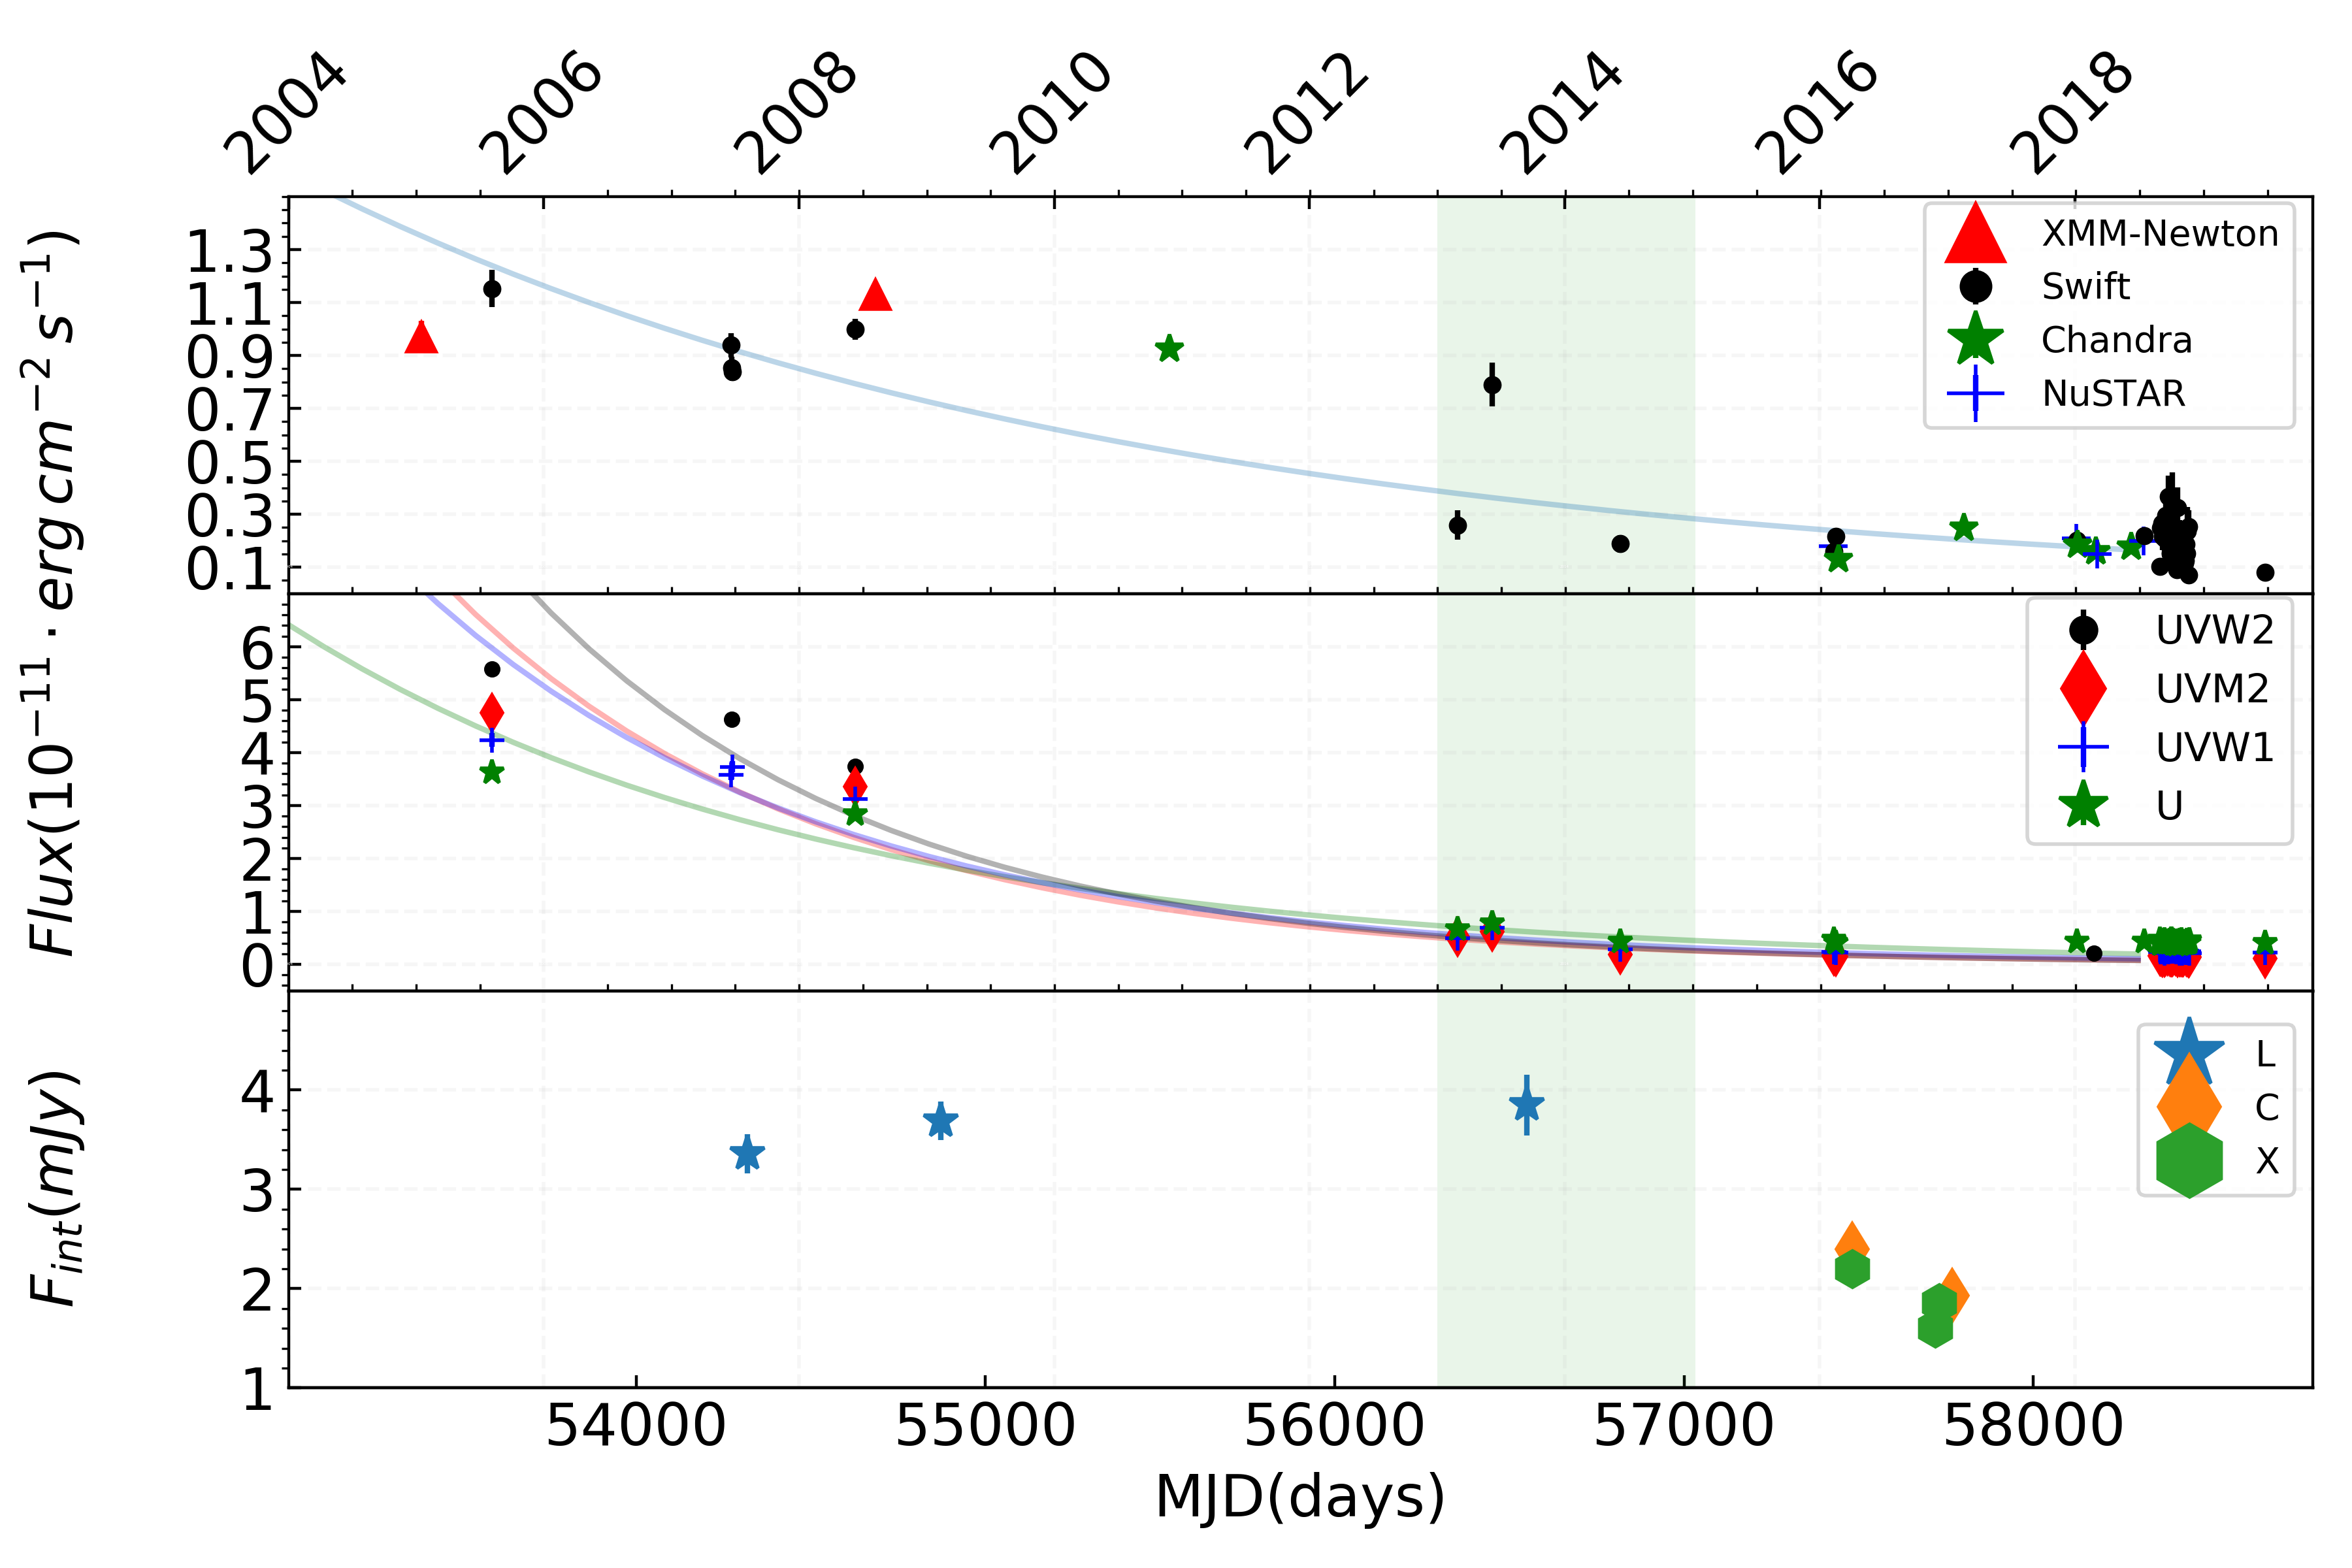
\includegraphics[width=0.9\textwidth]{./pic/subplots-xrt_uvot-radio-second.png}
    \caption{Multi-wavelength light curve of Mrk~1018 between 2005 and 2019. Red and blue vertical dotted line represents the last time of optical spectroscopic confirmation at type 1 and type 1.9, respectively. Region between them is marked as changing-look phase. Grey shallow region shows that the type transition occurred between 2013--2015 inferred by \citet{2017A&A...607L...9K} due to the rapid dimming of X-ray flux. Dashed lines in top and middle panel shows the fitting of light curve in X-ray and UV band between 2008 and 2015 with exponential decay function $F=S_0 e^{-(t-t_0)/\tau }$.  While in faint state after 2016, there is still rapid variability in X-ray, see also \autoref{fig:x-ray-uv-lc-rp-secondaxis} for details. At bottom panel, the label ``$F_\mathrm{5\,GHz}$'' marked with blank circles represent the radio flux re-scaled to 5 GHz. The whole radio light curve is shown in \autoref{fig:radio-lc}.}
    \label{fig:multi-lc-secondaxis}
\end{figure*}

%Colors represent different states as same as \autoref{fig:multi-lc-secondaxis}.

\begin{figure*}
\centering
	% To include a figure from a file named example.*
	% Allowable file formats are eps or ps if compiling using latex
	% or pdf, png, jpg if compiling using pdflatex
	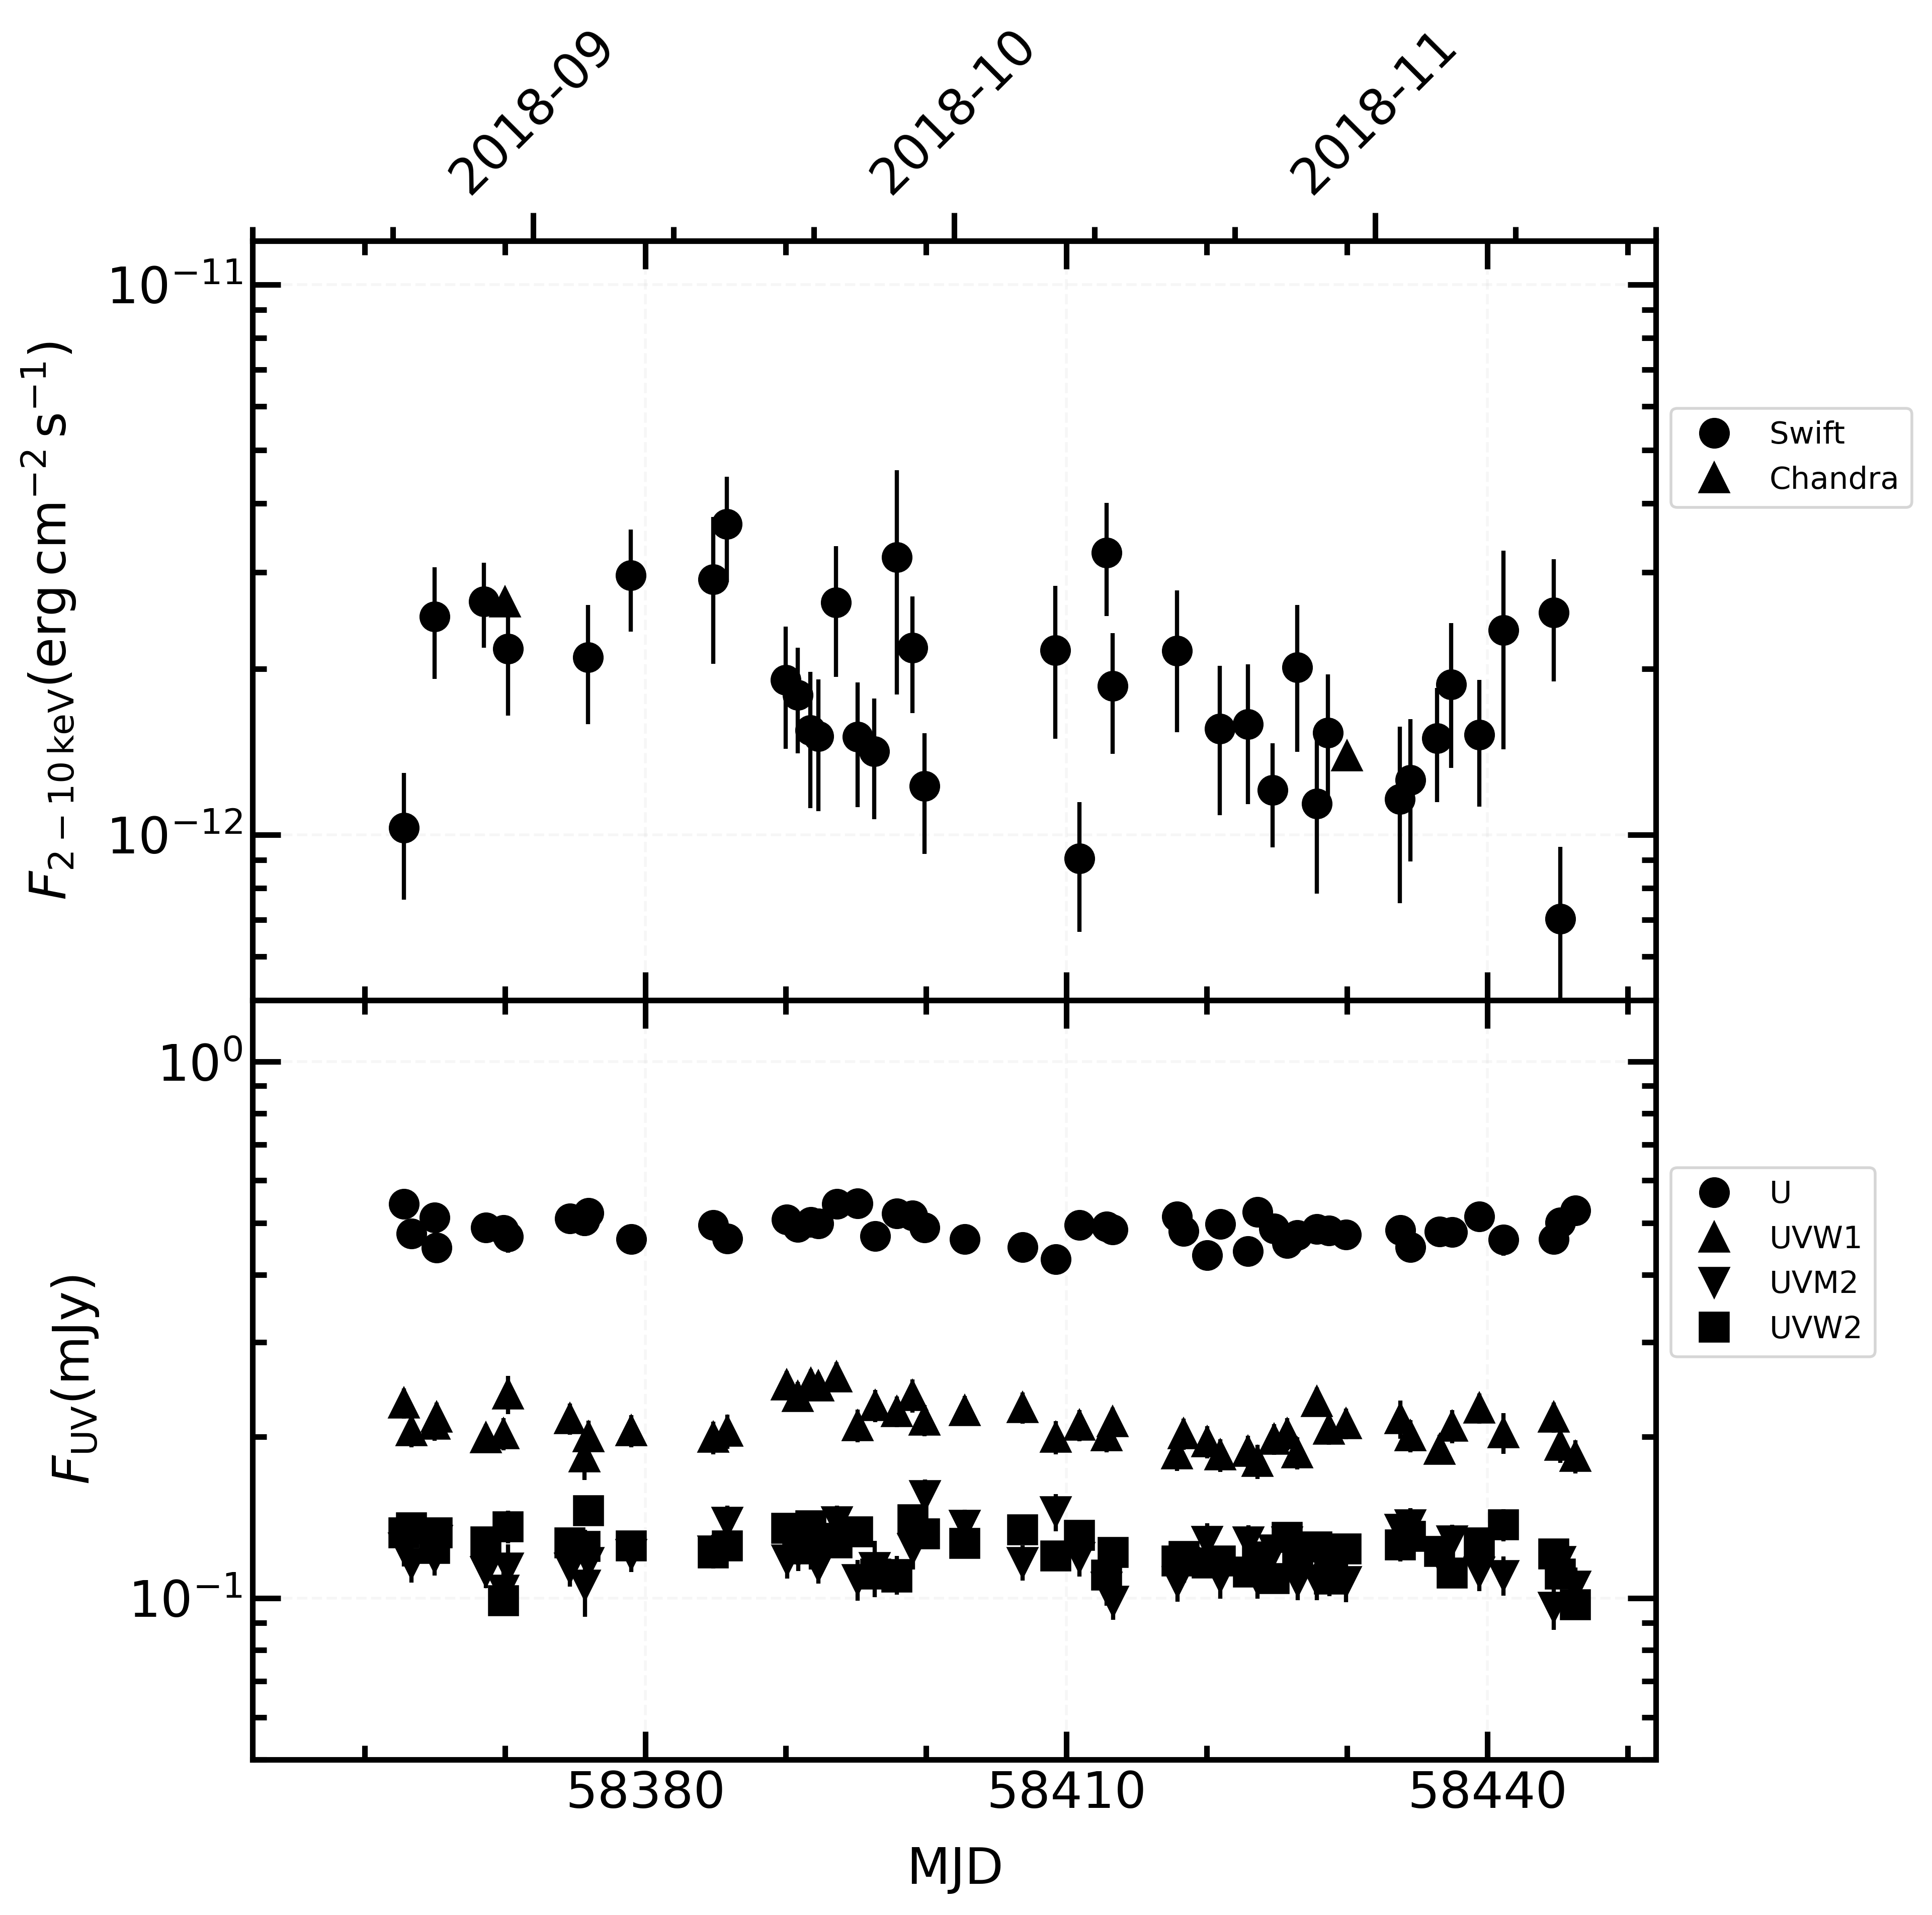
\includegraphics[width=\textwidth]{./pic/subplots-xrt_uvot-radio-second-right-part.png}
    \caption{Light curve of Mrk~1018 in X-ray and UV band with high-cadence monitoring observations between MJD 58350 and 58450.}
    \label{fig:x-ray-uv-lc-rp-secondaxis}
\end{figure*}

\begin{figure*}
\centering
	% To include a figure from a file named example.*
	% Allowable file formats are eps or ps if compiling using latex
	% or pdf, png, jpg if compiling using pdflatex
	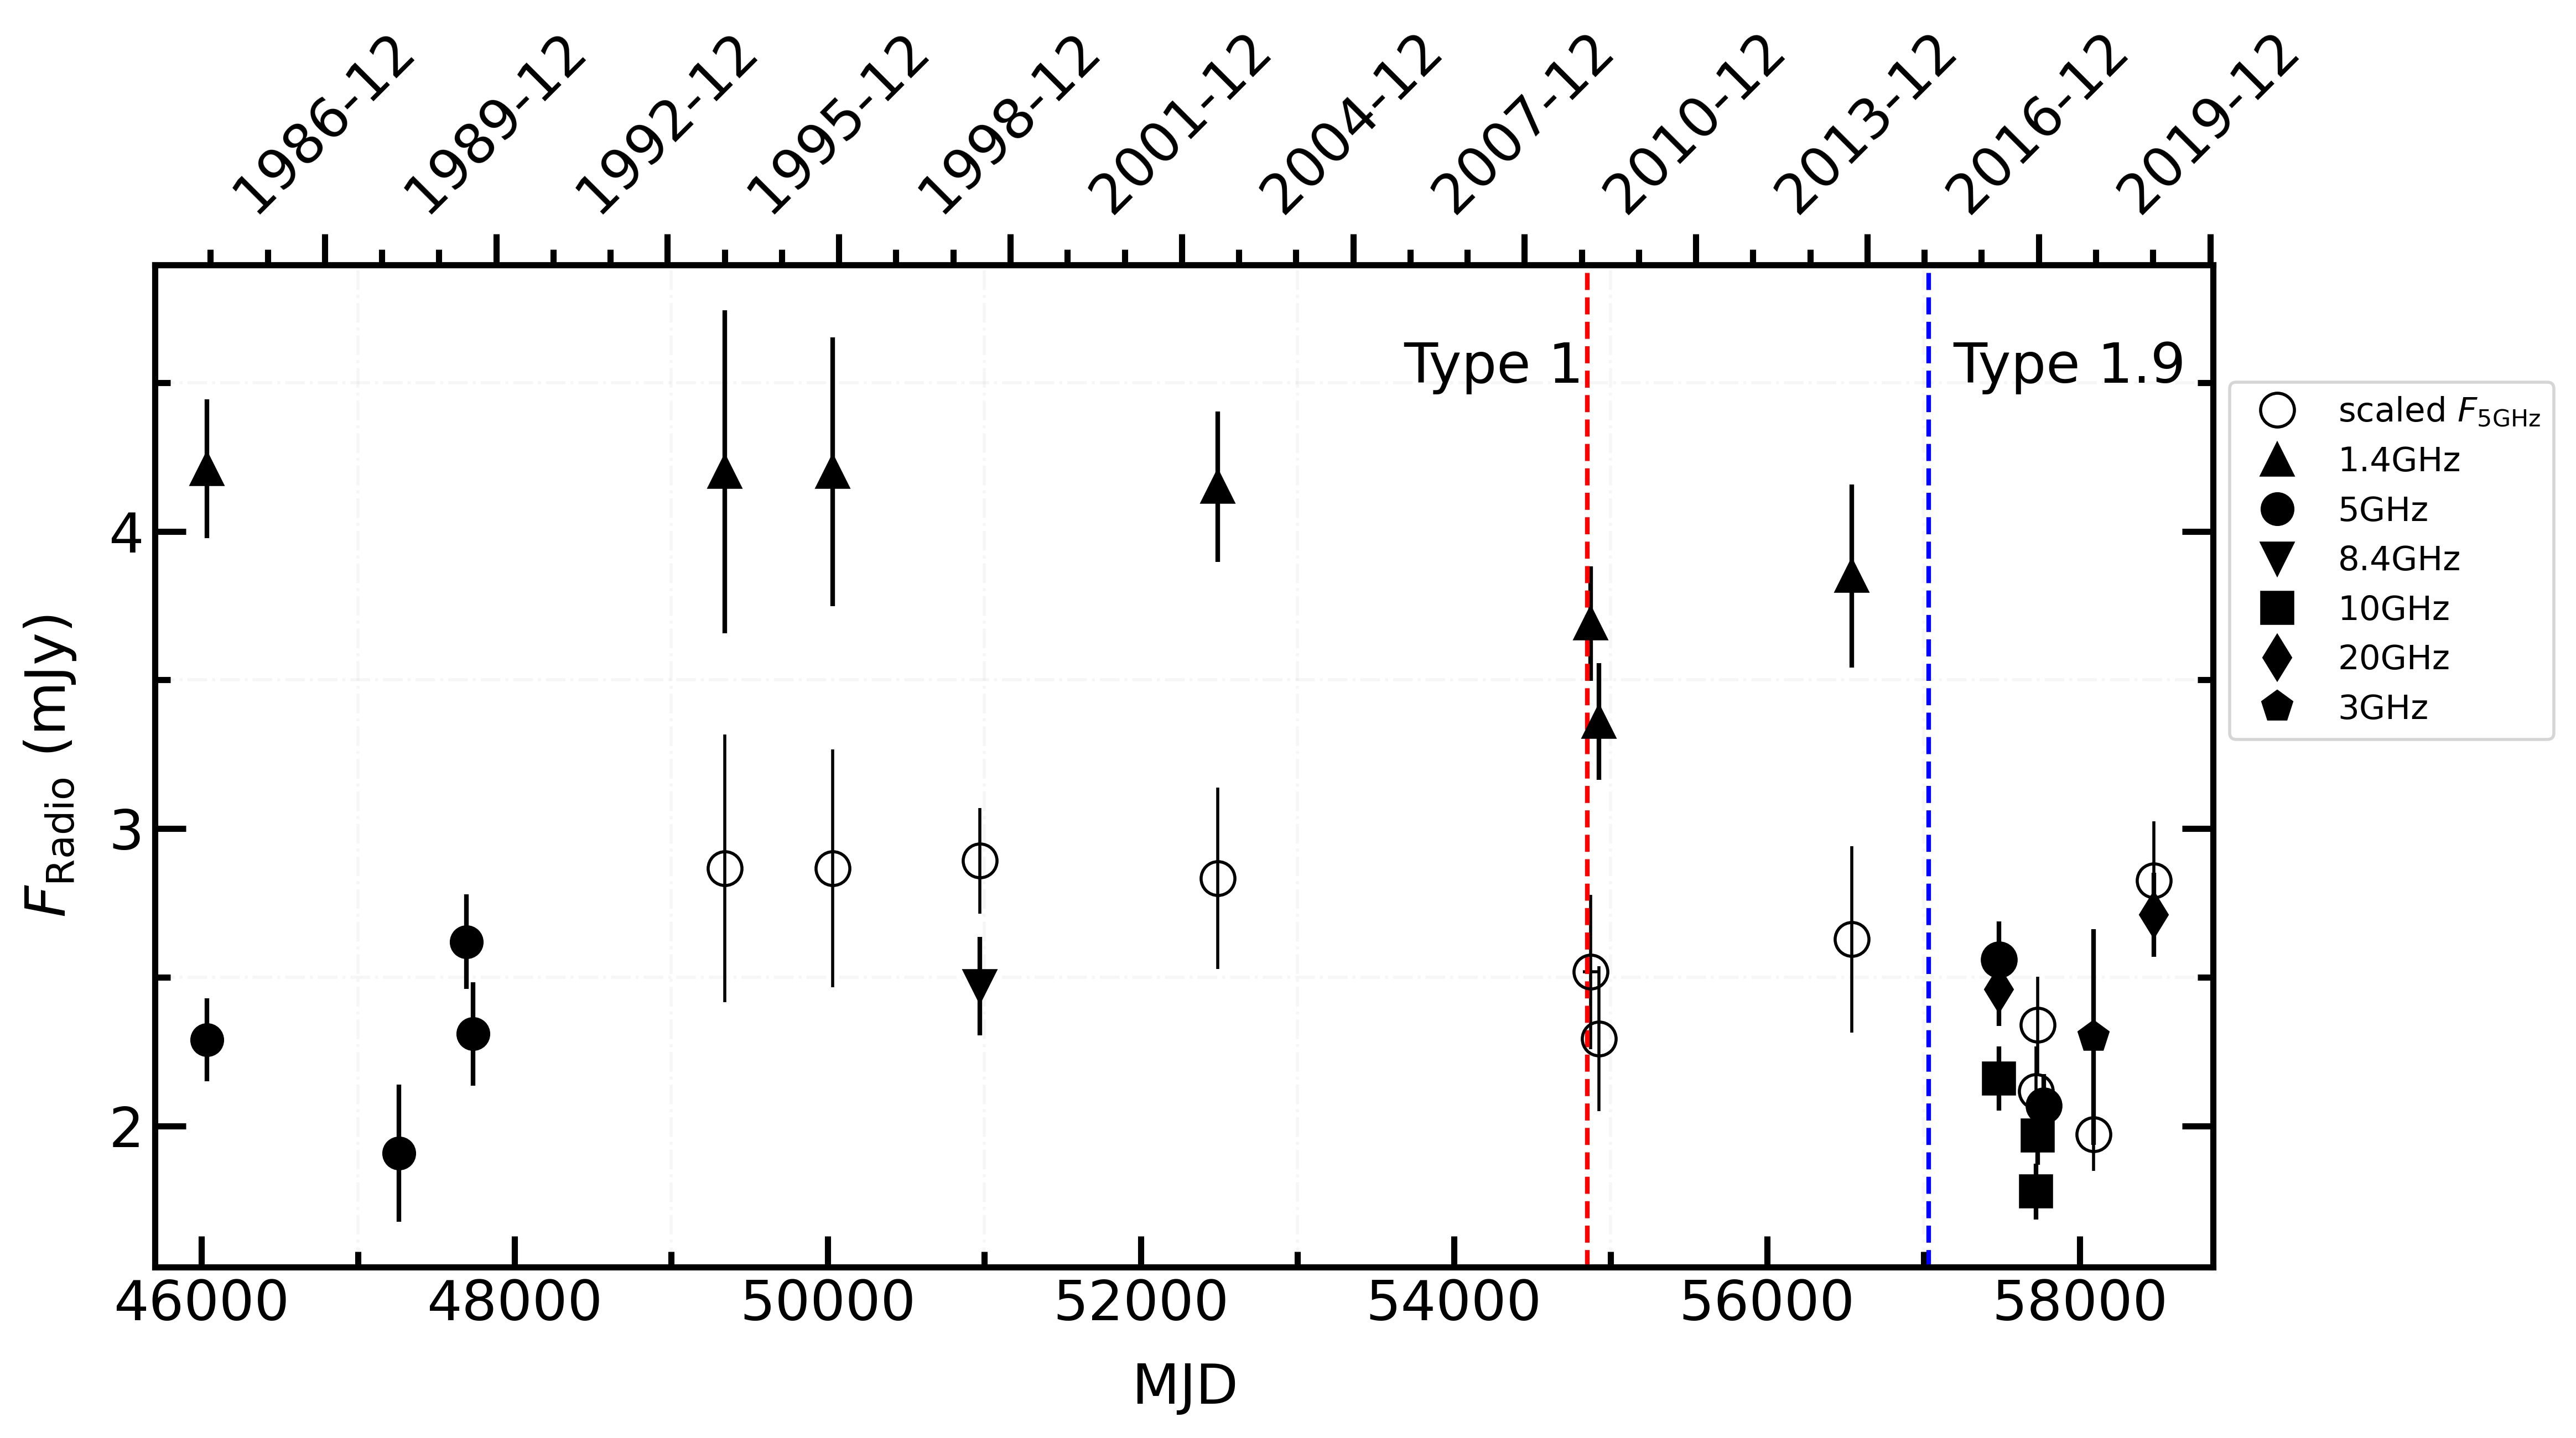
\includegraphics[width=\textwidth]{./pic/subplots-radio-second_freq.png}
    \caption{The whole radio light curve of Mrk~1018 with VLA observation. Filled markers represent the observation flux at corresponding frequency and blank circles represent the radio flux re-scaled to 5 GHz. Red and blue vertical dotted line represents the last time of optical spectroscopic confirmation at type 1 and type 1.9, respectively.}
    \label{fig:radio-lc}
\end{figure*}





 
Multi-wavelength light curves of Mrk~1018 are shown in \Cref{fig:multi-lc-secondaxis,fig:x-ray-uv-lc-rp-secondaxis,fig:radio-lc}. The flux in UV and X-ray bands in the whole roughly drops by a factor $\sim17.5$ and $\sim7.5$ during 2005--2016. However, the bolometric luminosity we estimate drops by a factor of $\sim24$. We find a good positive correlation between log$F_\mathrm{2-10\,keV}/L_\mathrm{Edd}$ and log$L_\mathrm{bol}/L_\mathrm{Edd}$, which is parameterised as 
\begin{equation}\label{Lbol-LX}
\mathrm{log} L_\mathrm{bol}/L_\mathrm{Edd}= 1.52 \times \mathrm{log} F_\mathrm{2-10\,keV}/L_\mathrm{Edd}+2.25.
\end{equation} The Spearman correlation coefficient of two quantities is 0.987 (pvalue=7.2e-07). So we use the correlation to derive other bolometric luminosities. It seems that flux in optical and X-ray band starts to decline around 2009 \citep[see also the optical light curve in ][]{2016A&A...593L...8M}. The rapid decay occurs during the changing-look phase. In order to roughly estimate the characteristic decay timescale, we then use an exponential function ($F=S_0\,e^{-(t-t_0)/\tau }$) to fit the X-ray and optical/UV light curves during MJD 54628-57033. The characteristic decay timescale $\tau$ is obtained as $\sim$1200, $\sim$1200, 900, 800, and 800 days for light curve in X-ray, U, UVW1, UVM2 and UVW2 band. During the changing-look phase($\sim 2009-2015$), we find there is a flare that brightness in X-ray and UV band increases by a factor $\sim3.2$ and $\sim1.4$ in 98 days and then drops by a factor $\sim4.2$ and $\sim2.5$ in 367 days. During the type 2 phase between MJD 58350 and 58450, there is still significant variability in X-ray band and relatively weaker variability in UV band. To quantify the normalized excess variance, we estimate $\sigma^2_{rms} $ defined in \citet{1999ApJ...524..667T} as
\begin{equation}
\sigma^2_{rms}=\frac{1}{N\mu^2}\sum_{i=1}^{N}[(X_i-\mu)^2-\sigma_i^2]
\end{equation}
The error on $\sigma^2_{rms}$ is $s_D/(\mu^2\sqrt{N})$, where \begin{equation}
s_D^2=\frac{1}{N-1}\sum_{i=1}^{N}\{[(X_i-\mu)^2-\sigma_i^2]-\sigma^2_{rms}\mu^2\}^2
\end{equation}

%f_uuu=(constants.c/(3465*units.AA)).to(u.Hz).value
%f_uw1=(constants.c/(2600*units.AA)).to(u.Hz).value
%f_um2=(constants.c/(2246*units.AA)).to(u.Hz).value
%f_uw2=(constants.c/(1928*units.AA)).to(u.Hz).value


We get $\sigma^2_{rms} = 0.0497 \pm 0.025 $ (corresponding to fractional variability with $\sim$20\%) from the X-ray light curve between MJD 58350 and 58450. The corresponding $\sigma^2_{rms}$ for U, UVW1, UVM2 and UVW2 band are 0.0003$\pm$0.0006, 0.0035$\pm$0.0015, 0.0036$\pm$0.0023, and 0.0034$\pm$0.0014, respectively. The variability is less significant in UVW1, UVM2 and UVW2 band and weak in U band compared to X-ray band during the faint state, which is consistent with the discussion above (see \autoref{sec:uvot}). These rapid variability with comparable amplitude are also seen in a sample of AGNs with \swift \, accretion disk reverberation mapping \citep[see ][]{2019ApJ...870..123E}.

%Radio
Radio flux in L and C band during type 1 phase keeps almost constant within errors. Flux in L band decreases by $\sim$44\% from MJD 52484 (type 1) to MJD 58087(type 2), while flux in C band decreases by $\sim$ 20 \% from MJD 57481 to MJD 57719 in type 2 phase. The flux in X band shows decrease first $\sim$17\% then slightly increase $\sim$10\% from MJD 57481 to MJD 57719 then on MJD 57731. The flux in K band shows slightly increase $\sim$10\% from MJD 57481 to MJD 58472 in type 2 phase. The whole light curve with re-scaled $F_\mathrm{5\,GHz}$ shows variability less than $\sim$40\% (see \autoref{fig:radio-lc}). 



\subsection{Correlation between X-ray and UV Luminosities}\label{subsec:xray-uv}
We use the simultaneous \xrt\, and \uvot\, data between MJD 53587 and 57430 to analyse the relation between X-ray and UV luminosity. X-ray flux shows a positive correlation with the UV flux during the changing-look phase (see \autoref{fig:correlation-Luvot-L2keV}). During the re-flare from MJD 56352 to 56450, the flux in U, UVW1, UVM2 and UVW2 band increases by a factor of 1.16, 1.38, 1.18 and 1.52, which is much smaller than the variability mentioned above in X-ray band, making the re-flare point the evident outlier (large than 2$\sigma$ deviation) in $L_\mathrm{{2\,keV}}$-$L_\mathrm{{UV}}$ diagram. When we exclude the outlier and re-fit the correlation parameterised as log $ L_\mathrm{{2\,keV}}$=$\gamma$ log $ L_\mathrm{{UV}}$+$\beta$. The slope $\gamma$ are 1.03, 0.74, 0.66 and 0.63, respectively. The Spearman correlation coefficient between simultaneous flux of \xrt\, and four \uvot\, band(U, UVW1, UVM2 and UVW2) are 0.99, 0.93, 0.90 and 0.89 (p-values are 1.4e-24, 2.5e-3, 0.037 and 0.018), respectively. But there is no evident correlation of X-ray/UV flux during the type 2 phase.

\subsection{Correlation between X-ray Luminosity and Photon Index}
The $\Gamma$-$L_{2-10\,keV}/L_\mathrm{Edd}$ diagram shows distinct anti-positive/positive correlation when $L_{2-10~ keV}/L_{Edd}$ (X-ray Eddington rate) below/above a critical value (~0.001), making the so-called ``V'' shape correlation, has been found in both AGNs and BH XRBs \citep[e.g.][]{2011A&A...530A.149Y,2015MNRAS.447.1692Y}. For Mrk~1018, $\Gamma$-$L_{2-10\,keV}/L_\mathrm{Edd}$ diagram shows evident anti-positive correlation when $L_{2-10\,keV}/L_{Edd}$ is below a critical value. But the positive correlation is less significant when $L_{2-10\,keV}/L_{Edd}$ is above the critical value since data points are limited. The data of Mrk~1018 roughly follows the two best-fitting lines with $\Gamma$= 1.05$\times$log$L_{2-10~ keV}/L_{Edd}$ +4.26 and $\Gamma$= -1.15$\times$log$L_{2-10~ keV}/L_{Edd}$ -1.98  when data points are divided into right and left branch based on luminosity. The Spearman correlation coefficient between photon index and X-ray Eddington rate is 0.2 and -0.57 (p-values are 0.58 and 4.3e-6) in right and left branches. We get similar results with slopes equal to 1.45 and -1.14 at positive and negative branch when fitting with a piecewise linear regression and derive that the critical value for log$L_{2-10~ keV}/L_{Edd}$ is $\sim$ -2.81, which is correspond to $L_\mathrm{bol}/L_\mathrm{Edd}\sim$1\% according to \autoref{Lbol-LX}. The best-fitting results in \citet{2015MNRAS.447.1692Y} are also included for comparison (see \autoref{fig:xrayappendgood-Lrateandg-tmap}). For a sample of AGNs, the critical value of -3 is close to our individual case, but the slopes (0.31 and -0.1) of positive and negative branch is much smaller. $\Gamma$ could be more efficiently regulated by the change of luminosity in individual source. Most of data on the positive branch roughly correspond to the type 1 AGN phase, while the negative branch roughly corresponds to the type 2 AGN phase. However, we find that it transits between two branches during the changing look phase (see \autoref{fig:xrayappendgood-fandg-tmap} and \autoref{fig:xrayappendgood-Lrateandg-tmap}). The X-ray flux increases by a factor $\sim3$ from MJD 56352 to 56450, while $\Gamma$ drops from $\sim1.8$ to $\sim1.4$, which makes it transits from negative branch to the positive branch, and then returns back to the negative branch on MJD 56817 when the X-ray flux decreases by a factor of $\sim$4.2, and $\Gamma$ does not vary. 

\subsection{Evolution of Broad-band Spectrum}
\label{subsec:xray-uvot-sed}
Broad band spectral energy distribution (SED) before and after the changing-look has been fitted \citep{2016A&A...593L...9H}. As the flux drops in X-ray and UV bands, the broad band SED also changes. We present the simplified \swift \, SED for Mrk~1018 in \autoref{fig:sed}. Then we use simultaneous XRT and UVOT data to explore the evolution of broad band SED with {\it optxagnf} plus {\it hostpol} model. We find that bolometric luminosity could be constrained well even though soft Comptonisation component parameters $r_\mathrm{cor}$ and $T_\mathrm{disk}$ could not be well constrained (see also detailed text in \autoref{data-xrt}). We present the evolution of disk temperature derived from standard thin disk model in \autoref{fig:disk_evoliton}, which is consistent with the drop of the disk temperature from type 1 to type 1.9 state \citep[also described in][]{2016A&A...593L...9H}. The disk temperature is modulated by the $L_\mathrm{bol}$ and $r_{cor}$. During the changing-look phase, the flare points shows high value of $r_{cor}$ as luminosity increases and spectrum becomes hard, and then return to low $r_{cor}$ as luminosity declines and spectrum does not vary. But the large errorbar of $r_{cor}$ might be not enough to ascertain the variation during the period.

\begin{figure*}
\centering
	% To include a figure from a file named example.*
	% Allowable file formats are eps or ps if compiling using latex
	% or pdf, png, jpg if compiling using pdflatex
	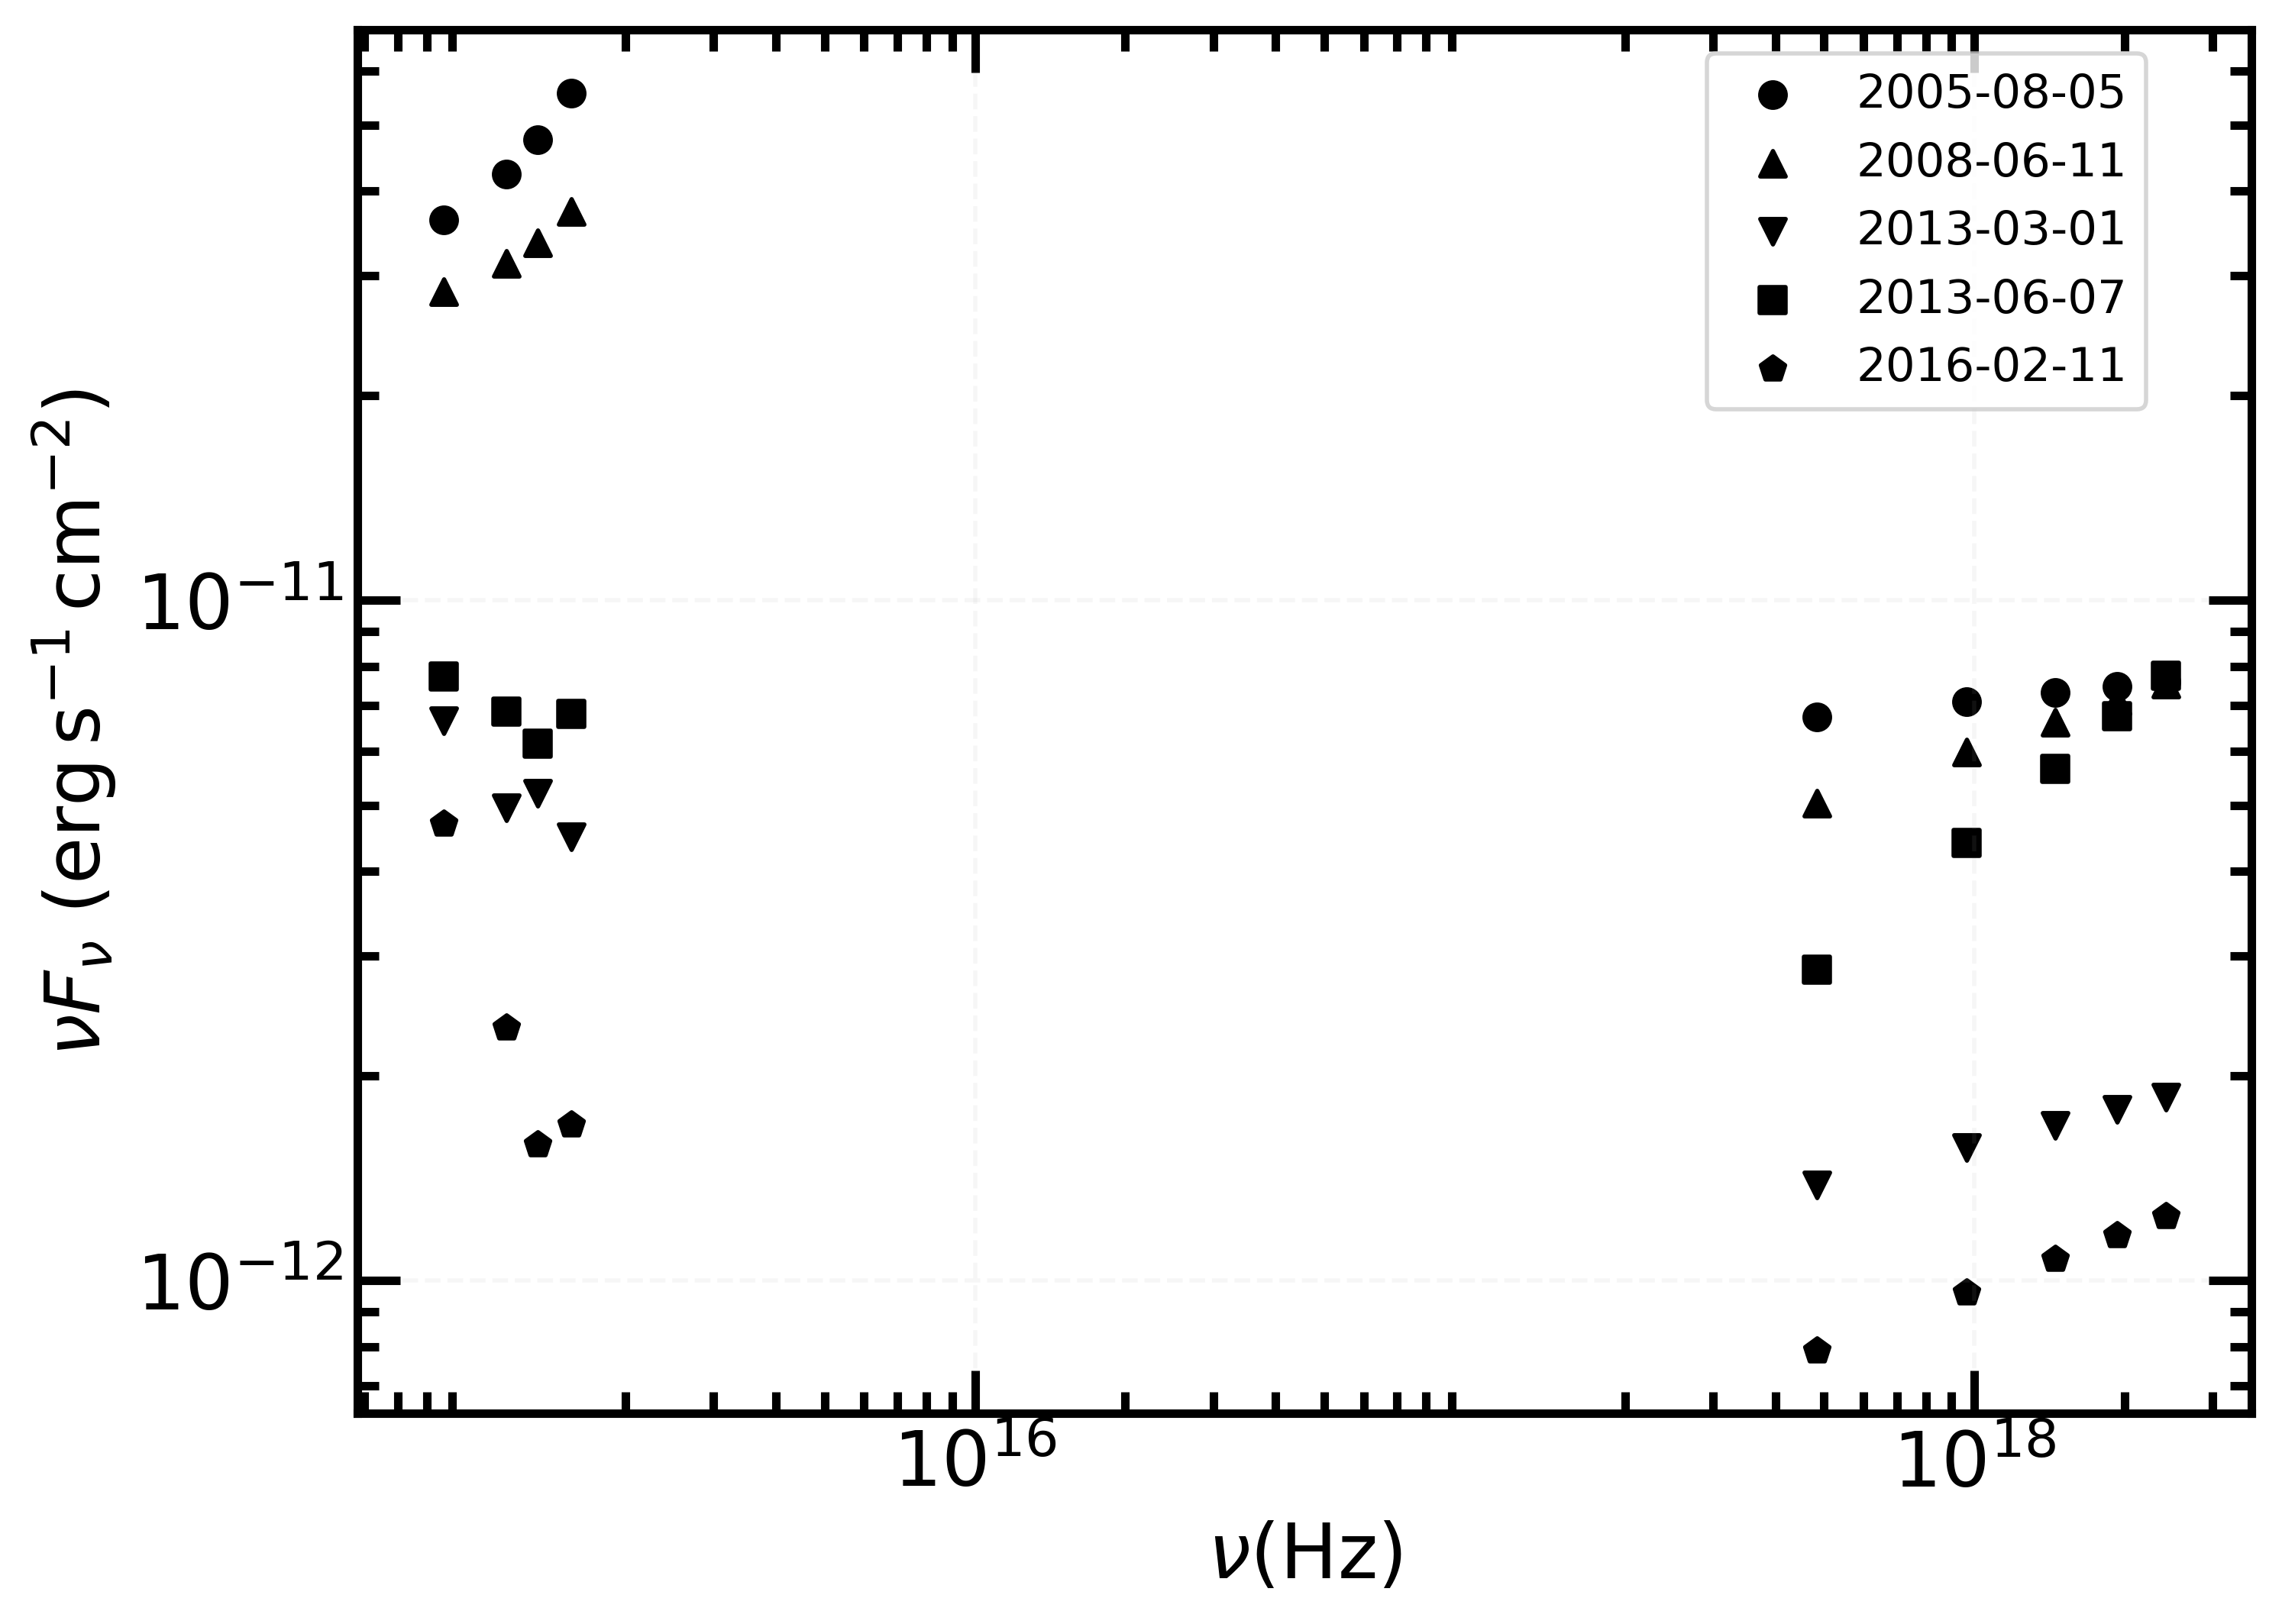
\includegraphics[width=0.9\textwidth]{./pic/Mrk1018_sed_date.png}
    \caption{\swift \, SED of Mrk 1018. We adopt five points for X-ray spectrum based on absorbed power-law model for illustration. The peak frequency of UV spectrum shift to left and the photon spectral index of X-ray also varied with time.}
    \label{fig:sed}
\end{figure*}

 \alphaox \,is also a good indicator of the broad SED, which has been used extensively for a long time \citep[e.g.][]{1979ApJ...234L...9T}. Here we define \alphaox as 
%\begin{equation}
%\alpha_{OX}  = - \frac{\log(\lambda F_{2600 \angstrom}/\nu F_{2keV})}{\log(\nu_{ 2600 \angstrom }/\nu_{2keV})}+1
%\end{equation}
\begin{equation}
\alpha_{OX} = \frac{\log (L_\mathrm{UV} / L_\mathrm{X} )} {\log (\nu_\mathrm{X} /  \nu_\mathrm{UV} )}=\frac{\log (L_\mathrm{UV} / L_\mathrm{X} )}{2.623}
\label{definition_alpha_ox}
\end{equation}
, where the $L_\mathrm{UV}$ is from the UVW1 filter with central wavelength {2600{$\angstrom$}} and full-width at half max of $\sim 683\angstrom$ \citep{2008MNRAS.383..627P} and the $L_\mathrm{X}$ is the luminosity at 2 keV, which are consistent with previous literature. We derive the flux at 2 keV from $F_{2-10~ keV}$ and  photon index $\Gamma$ based on the power-law fitted spectrum. \alphaox-$L_\mathrm{UV}$ vs. \alphaox-$L_\mathrm{X}$ is shown in \autoref{fig:alpha_ox_lx_luv}. We should notice that the intrinsic AGN emission should be weaker in UV band due to the host galaxy contamination. 



\section{Discussion}\label{sec:discussion}
\subsection{Spectral Evolution and Changing-look}
\label{sec:spectral evolution}
We find that the correlation between the X-ray photon index $\Gamma$ and the X-ray luminosity $L_\mathrm{X}$ roughly follows a ``V"-shaped (see \autoref{fig:xrayappendgood-fandg-tmap}). Recently, this correlation has also been found in a sample of CL-AGNs \citep[e.g.][]{2019arXiv191203972L}. The case of Mrk 1018 demonstrates that the ``V"-shaped correlation between $L_\mathrm{X}$ and $\Gamma$ also holds in individual source \citep[see also in ][etc]{2020ApJ...890L..29A}. Similar phenomenon has also been observed in normal AGNs (relative to CL-AGNs) over a large luminosity range \citep[e.g. ][]{2009MNRAS.399..349G, 2011A&A...530A.149Y}. It is interesting to notice that the pivoting points of the ``V"-shaped correlations of CL-AGNs and normal AGNs show almost the same value of  $\sim 10^{-3}~L_\mathrm{2-10 keV}/L_\mathrm{Edd}$. It is well known that the X-ray emission of an AGN is from the Compton scattering in the hot corona \citep[e.g.][]{1991ApJ...380L..51H}. In the normal AGNs, the reason for the opposite X-ray spectral behavior is thought to be the differences of the seed photons for the Compton scattering, i.e. the seed photons are from the synchrotron emission of the hot corona itself at the low luminosity branch, while are from the thermal emission from Shakura–Sunyaev disc \citep[SSD; e.g. ][]{2013ApJ...764....2Q} or other thermal component \citep{2015MNRAS.447.1692Y} at the high luminosity branch. So the same mechanism should also work in Mrk 1018, i.e. an extra thermal component (such as SSD) which provides the external seed photons appear (disappear) above (below) the critical luminosity in addition to the hot corona. 

Another parameter \alphaox\, is found to be positively correlated with the luminosity in different luminous AGNs samples \citep[e.g.][]{2010A&A...512A..34L, 2013A&A...550A..71V,2016ApJ...819..154L}, and negatively correlated with the luminosity in the low luminosity AGNs \citep{2011ApJ...739...64X,2017MNRAS.471.2848L}. The dividing point of these two opposite correlations is roughly at $10^{-3}$--$10^{-2}~L_\mathrm{Edd}$ \citep{2011ApJ...739...64X,2017MNRAS.471.2848L}. The hot accretion flow is thought to dominate the broad band emission from optical to X-ray in the LLAGNs \citep[see reviews in ][]{2014ARA&A..52..529Y}. While the X-ray is from Compton scattering of the hot corona, and the optical/UV emission originates from the SSD in the luminous AGNs. At the same time, the hot accretion flow can well explain the negative correlation between \alphaox and $L_\mathrm{bol}$ at the low luminosity branch \citep{2011ApJ...739...64X,2017MNRAS.471.2848L}, and the disk-corona can explain the positive correlation of them at the high luminosity branch \citep{2017A&A...602A..79L, 2018MNRAS.480.1247K,2019A&A...628A.135A}. The different relations between \alphaox and $L_\mathrm{bol}$ clearly supports the idea that the accretion mode changes in the high and low luminosity AGNs \citep{2011MNRAS.413.2259S,2019ApJ...883...76R}. 

Mrk~1018 similarly follows the ``V"-shaped correlations in $\Gamma$--$L_\mathrm{X}$ diagram, which supports the idea that the accretion mode changes as the luminosity decreasing below the critical value. \citet{2018MNRAS.480.3898N} have fitted the broad band SEDs of Mrk 1018 at high, median and low luminosity are also found the accretion mode changes as the luminosity decreasing. Actually the ``V"-shaped $\Gamma$--$L_\mathrm{X}$ correlation also exists in the BHXRBs, and is well explained by the same mechanism to AGNs\citep[e.g.][]{2011A&A...530A.149Y,2015MNRAS.447.1692Y}. \citet{2011MNRAS.413.2259S} simulated the spectral states of AGNs by analogy with BHXRBs, and found that the simulated AGNs at different spectral states and luminosities roughly follow a ``V"-shaped \alphaox--$L_\mathrm{bol}$ correlation \citep[see also in ][]{2019ApJ...883...76R}. \citet{2019arXiv190904676R} recently finds two CL-AGNs follow a roughly ``V"-shaped \alphaox--$L_\mathrm{UV}$ correlation, although they applied an X-ray reprocessing model to explain the correlation. We also plot the \alphaox and $L_\mathrm{X}$ by using their data. It seems that they follow two negative correlations with different slopes for type 1 and type 2 AGNs. The shapes of the two correlations \alphaox-$L_\mathrm{X}$ and \alphaox-$L_\mathrm{UV}$ are apparently different. The pivoting luminosity differs from \citet{2011ApJ...739...64X} by almost one order of magnitude. So here is an issue about the bolometric correction of $L_\mathrm{X}$ or $L_\mathrm{UV}$ with a large dynamic range of \alphaox and luminosity. 

 However, we find that there is evident positive correlation between $L_\mathrm{X}$ and $L_\mathrm{UV}$ of Mrk~1018 during the changing-look phase. According to \autoref{definition_alpha_ox}, if the non-linear relationship between $ L_{\mathrm{X}}$ and $ L_\mathrm{UV}$ is parameterised as log $L_\mathrm{X}$ = $\gamma $ log $L_{\mathrm{UV}} $ +$\beta$, we derive that $\alpha_{OX}\propto (\frac{1}{\gamma}-1) \log L_\mathrm{X}$, and $\alpha_{OX}\propto (1-\gamma) \log L_\mathrm{UV}$. With $\gamma$ =0.745 (see \autoref{subsec:xray-uv}), $\alpha_{OX}$ should be linearly correlated with $\log L_\mathrm{X}$ and $\log L_\mathrm{UV}$ with slope 0.34 and 0.26, respectively. So the data of Mrk~1018 should not show two branches, which may need more samples for further investigation. Interestingly, Mrk~1018's position in the \alphaox-$L_\mathrm{UV}/L_\mathrm{Edd}$ and \alphaox-$L_\mathrm{2\,keV}/L_\mathrm{Edd}$ is well in agreement with type 1 and type 2 branches when we add the data of Mrk~1018 on the plots of two CL-AGNs in \citet{2019arXiv190904676R} (see \autoref{fig:alpha_ox_lx_luv}).
 
%$\gamma$ =0.745 which is consistent with the correlation found in quasars \citep[see ][]{2016ApJ...819..154L}.
%It is thought to be similar to the state transition behavior in the Galactic black hole X-ray binaries (BHXRBs). 




%\textcolor{red}{}
The accretion mode changes have also been suggested in other CL-AGNs or highly variable AGN \citep{2019arXiv191203972L,2020ApJ...890L..29A,2020MNRAS.492.2335L}. However the link between accretion mode changes and the AGN type transitions are still not fully understood. It has been observed that the broad line luminosity is positively correlated with the UV luminosity, and the broad line width is negatively correlated with the UV luminosity \citep[e.g.][]{2019ApJ...885...44D}. So in our case of Mrk 1018, if the inner disc disappears at the low luminosity, which is consistent with the decreasing of the disc temperature \citep[see also ][]{2018MNRAS.480.3898N}, the reduced UV luminosity will cause the broadened line component non-detected. On the other hand, some models of the broad line region are indeed related with the SSD, which can be account for the type transition in the CL-AGNs \citep[see a recent review in ][]{2019OAst...28..200C}. For example, in the disk-wind model of the BLR origin, the AGNs evolve from type 1 to type 2 as the luminosity decreasing \citep[see][]{2014MNRAS.438.3340E}. \citet{2018MNRAS.480.3898N} suggests that the soft X-ray excess contributes most ionizing photons, and the drop of soft X-ray excess causes the disappearance of broad emission line \citep[see also in ][]{2020MNRAS.492.2335L}. However, the origin of the soft excess is still under debate \citep[e.g.][]{2018A&A...611A..59P}, which is worthy to further study in CL-AGNs. 


%\textcolor{red}{}


 




\subsection{Long and short-term variabilities}

We derive three characteristic timescales when Mrk~1018 transited from type 1 to type 1.9 with rapid dimming of luminosity. The UV/optical and X-ray luminosity roughly decrease by a factor of 7.5 and 17.5 within 10 years. The corresponding exponential decay timescale is $\sim$ 800--1200 days from 2009 to 2015 as Mrk~1018 transited from type 1 to type 1.9. Besides, the timescale for Mrk~1018 to be located at different branch of $\Gamma$--$L_\mathrm{X}$ diagram could be as short as 100 days, which is also the re-flare timescale. Such re-brightening within several tens to hundreds of days is also found in some other CL-AGNs \citep[e.g.][and references therein]{2017MNRAS.467.1496O,2019MNRAS.487.4057K,2020MNRAS.498..718O}. Due to the high-cadence monitoring observations, we also found that the X-ray luminosity vary dramatically on timescale of tens of days (see \autoref{sec:multi-lc}). What mechanisms drive such long and short-term flux variations are still unknown. 

The flux variations of AGNs on different time scales and different wavelengths have been studied for a long time \citep[see reviews in ][]{1997ARA&A..35..445U}. A damped random walk (DRW) process provide a good description of AGN variabilities on timescales of days to years \citep[e.g.][]{2010ApJ...721.1014M,2011ApJ...730...52K}, which could be driven by the variations in the magnetic field of the accretion flow \citep{2004MNRAS.348..111K,2006MNRAS.368..379M,2007A&A...466..793J}. \citet{2004MNRAS.348..111K} has demonstrated that the model can produce small flux fluctuations and also stochastic large flares. It seems to be a promising explanation for the long and short variability of changing-look AGNs like Mrk~1018. As we discuss in \autoref{sec:spectral evolution}, the critical luminosity for accretion mode changes is roughly in the range $10^{-3}-10^{-2}L_\mathrm{Edd}$ \citep[see also ][]{2019arXiv191203972L}. If the AGN type transition indeed associates with the accretion mode changes, the AGNs at the luminosity level $10^{-3}-10^{-2}L_\mathrm{Edd}$ would be the candidates of changing-look AGNs, since the stochastic variation easily makes the luminosity above/below the critical luminosity to change the accretion mode. 

\citet{2018MNRAS.480.3898N} has made an analogy between the broad band spectral evolution of Mrk~1018 and the soft-to-hard state transition during the decay phase of BH X-ray transient. However, the decay timescale is still an issue for this analogy, since the decay timescale of an outburst of BH X-ray transient corresponds to the viscous timescale of outer accretion disc with $r_\mathrm{disk}\sim 1000\, R_g$(also see the discussions in \autoref{sec:spectral evolution}). Scaling to a $10^{8}M_{\odot}$ BH, the viscous timescale is roughly one million years \citep{2012MmSAI..83..469L,2018MNRAS.475.1190Y}, which is much longer than characteristic decay timescale we got in Mrk~1018. However, there are few cases that the spectral transition in BH XRBs occurs within few hours or even less \citep{2011A&A...533A...8B,2020A&A...634A..94K} during a highly variable period, the mechanism of this kind of rapid spectral transition is still unknown. 

\begin{figure*}
\centering
	% To include a figure from a file named example.*
	% Allowable file formats are eps or ps if compiling using latex
	% or pdf, png, jpg if compiling using pdflatex
	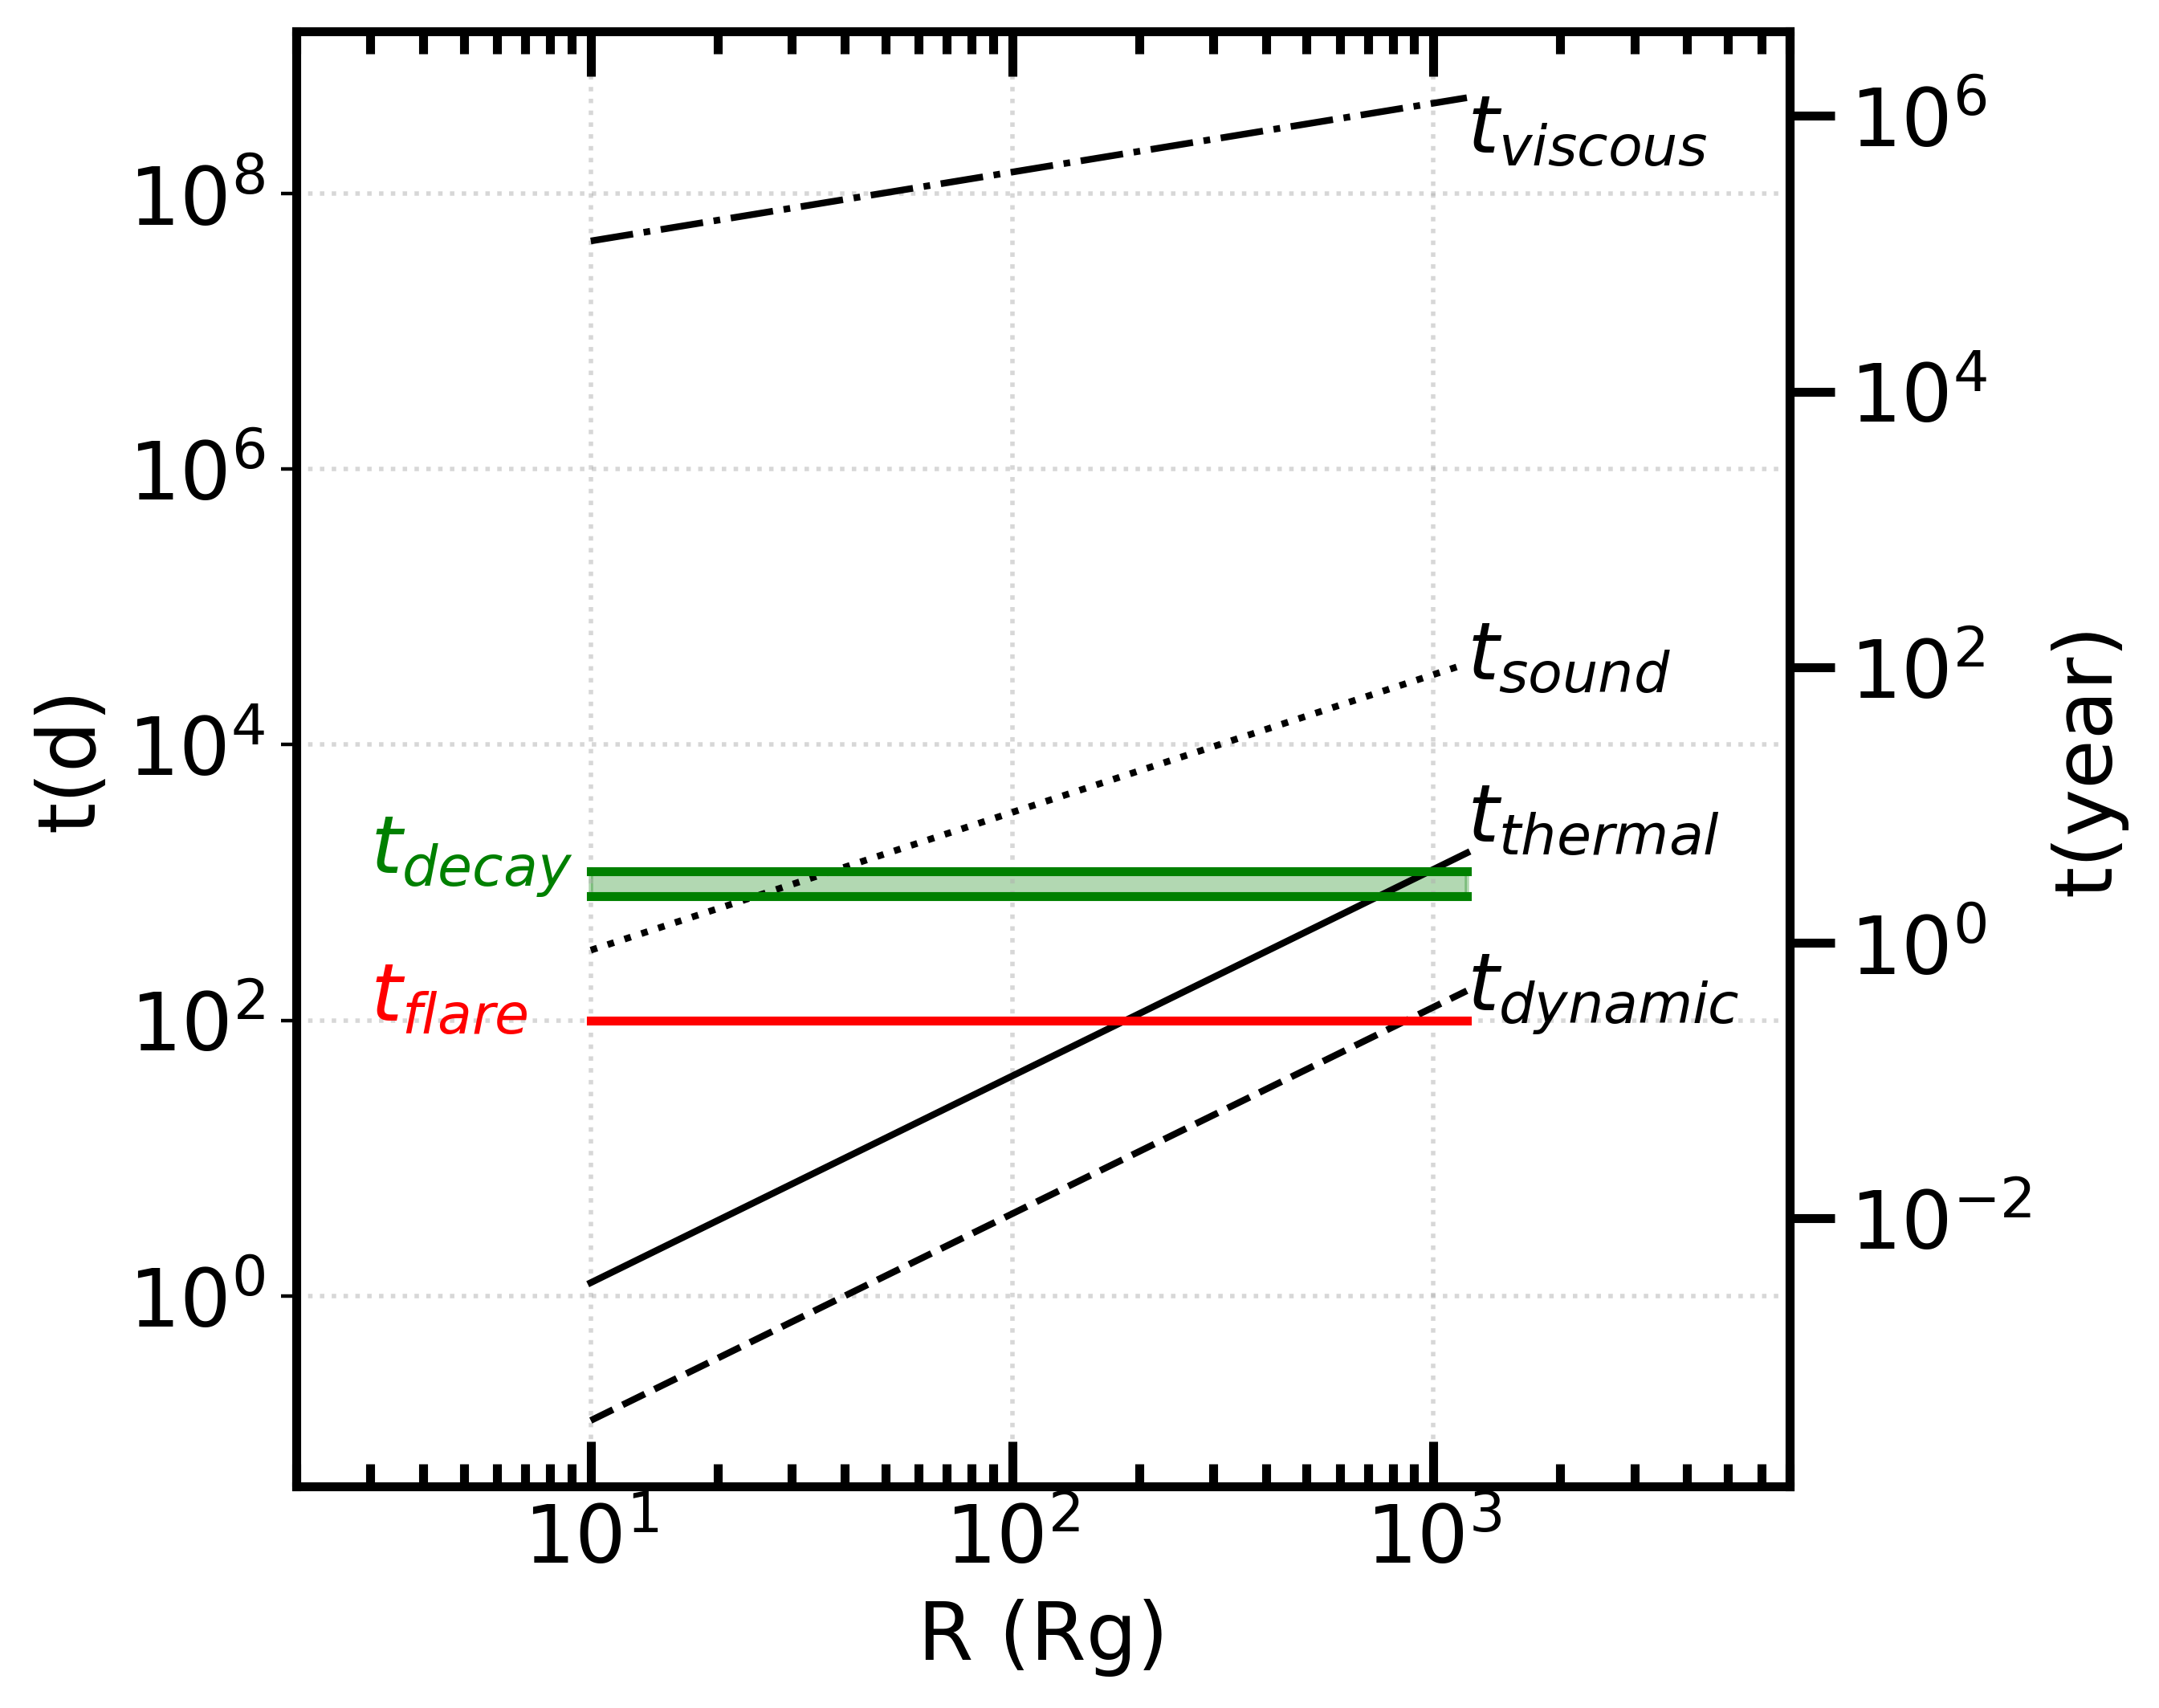
\includegraphics[width=0.8\textwidth]{./pic/Mrk1018_timescale.png}
    \caption{Different timescales on different radius correspond to viscosity timescale $t_\mathrm{vis}$, dynamical timescale $t_\mathrm{dy}$, thermal timescale $t_\mathrm{th}$ and sound crossing timescale $t_\mathrm{sound}$. Here we adopt typical value for $T_\mathrm{disk}=3\times10^4\, K$. Two horizontal lines correspond to exponential decay timescale $t_\mathrm{decay}$ $\sim$800-1200 days and flare timescale $t_\mathrm{flare}$ $\sim$ 100 days, which correspond to thermal timescale at $\sim$1000 and $\sim$ 200 $R_g$, respectively.}
    \label{fig:timescale}
\end{figure*}


Recently, more and more studies show that the behavior of CL-AGNs somehow are quite similar to the spectral state transitions in Galactic BHXRBs, and the mechanism caused the spectral state transitions in BHXRBs should also work in the CL-AGNs. However, this will bring a serious issue about the time scale, which has been noticed by previous works \citep[e.g. ][]{2018NatAs...2..102L,2018ApJ...864...27S,2018MNRAS.480.3898N,2020MNRAS.492.2335L}. The state transtions in BHXRBs normally occur on timescale of days to tens of days \citep{2009ApJ...701.1940Y,2010MNRAS.403...61D}, which is thought to corresponds to the viscous timescale of the truncated disc \citep[see reviews in ][]{2007A&ARv..15....1D}, where the viscosity timescale $\tau_{vis}$ is given as
\begin{equation}
\tau_{vis} \sim 5.7\times 10^{-3} \alpha^{-1}(\frac{M_\mathrm{BH}}{10^8M_{\odot}})(\frac{r_{tr}}{R_g})^{3/2} (\frac{H}{R})^{-2} \, days
\end{equation} It will be 3.9$\times 10^5$ years for Mrk~1018 if we adopt the truncated radius $r_{tr}$ at 100 $R_g$, viscosity coefficient $\alpha=0.1$ and disk height would be $H/R~\sim 5\times10^{-4}$ \citep[see also][]{2018MNRAS.480.3898N} in a thin disk scenario. Current observations show that the AGN type transition usually occurs on timescale of few years \citep[e.g.][]{2016A&A...593L...8M,2018ApJ...864...27S,2019MNRAS.483L..88P,2020MNRAS.492.2335L} or even few months \citep{2019ApJ...883...94T}. So different models are proposed to shorten the timescale, such as a thick disk support by the magnetic pressure \citep{2019MNRAS.483L..17D}, the radiation pressure instability at the boundary of ADAF \citep{2019arXiv190406767S} and the thermal timescale of the disk heating or cooling front \citep{2018ApJ...864...27S}. The thermal instability timescale $\tau_{th}$ is given as
\begin{equation}
\tau_{th} \sim \frac{\tau_{dy}}{\alpha} \sim 5.7\times 10^{-3} \alpha^{-1}(\frac{M_\mathrm{BH}}{10^8M_{\odot}})(\frac{r_d}{R_g})^{3/2} \, days
\end{equation}

Besides, \citet{2018ApJ...861...51K} consider the tidal impulse effect within a recoiling-SMBH scenario to explain the long-term variability. The sound crossing timescale $\tau_{s}$ caused by density perturbation is given as
\begin{equation}
\tau_{s}= 0.07 (\frac{M_\mathrm{BH}}{10^8M_{\odot}})(\frac{r_d}{R_g}) (\frac{T}{10^5 K})^{-1/2} \, years
\end{equation}  We plot the different timescale as function of radius (R) in \autoref{fig:timescale} as summary, but we still cannot really solve the timescale problem yet. 



\subsection{Correlation between radio and X-ray luminosities}
There is a non-linear correlation between the radio and X-ray luminosities (R-X correlation hereafter) spanning over different mass black holes from the super-massive black holes to stellar mass black holes, where the $L_\mathrm{R}$ is proportional to $L_\mathrm{X}^{0.6}$ \citep{2003MNRAS.345.1057M,2004A&A...414..895F}. However, there are some sources follow a steeper R-X correlation with a power-law index of $\sim$1.4 at high $L_\mathrm{X}$, a flat R-X correlation with a power-law index of  $\sim$0 at moderate $L_\mathrm{X}$, and the standard R-X correlation with a powerlaw index $\sim$0.6 \cite[e.g. ][]{2011MNRAS.414..677C,2016MNRAS.463.2287X} at low luminosity. The physics of this ``hybrid" R-X correlation is still under debate. The change of the correlation slope may attribute to the different accretion modes or jet physics at low and high luminosities\citep{2016MNRAS.456.4377X,2018MNRAS.481.4513I,2018MNRAS.473.4122E}. 

People usually use the radio luminosity at 5 Ghz and the 2--10 keV X-ray luminosity to investigate the R-X correlation. In order to keep consistent with previous literature, we use the radio spectral index to calculate the monochromatic radio luminosity at 5 GHz when this observation is not performed at 5 GHz (see the details in \autoref{subsec:vla}). The radio luminosity at 5 GHz only varies about 40\%, while the X-ray luminosity varies roughly one order of magnitude during the same time interval from MJD 53587 to 58430 (see \autoref{fig:multi-lc-secondaxis}). We plot the radio luminosity and the nearest X-ray luminosity (interval $\le$ 100 days, see \autoref{tab:radio_xray}) in \autoref{fig:radio-xray-mass_relation_Plotkin2012} and the best-fitting result of a sample of black holes with flat/inverted radio spectra index in \citet{2012MNRAS.419..267P}. Our current data shows that Mrk 1018 apparently does not follow the standard $L_{R}\propto L_\mathrm{X}^{0.6}$ correlation. It roughly follows a flat R-X correlation at the X-ray luminosity range 3$\times 10^{-4}$ to 4$\times 10^{-3}$ $L_\mathrm{Edd}$, which is similar to the flat part of the ``hybrid" correlation in BH XRBs ($10^{-3}$ to $10^{-2}~L_\mathrm{Edd}$) \citep[see e.g. ][]{2018MNRAS.473.4122E,2020ApJ...891...31X}. We also superimpose the data points of Mrk~590 from \citet[][]{2016MNRAS.460..304K} onto the plot since they share many similarities as CL-AGN. Both of them show type change from type 1 to type 2/1.9 within years. The ratio of radio and X-ray luminosity log$L_R/L_X$ is $\sim$ -5 to -4 for Mrk~1018 and Mrk~590. The latter is considered to be in accreting in a radiatively inefficient mode of low/hard state since Mrk~590 well follows the fundamental plane defined in a sample of low/hard state galactic black holes plus LINERs \citep[see ][]{2016MNRAS.460..304K}. Coincidently, the radio spectrum index ($\alpha_R$) for two sources both show the tendency to be flatter and several tens percent of decline in radio flux as the bolometric luminosity decline by around an order of magnitude. Besides, systematic distributional difference of $\alpha_R$ also exists in radio quiet AGN of different types \citep[e.g.][]{2019MNRAS.485.3185C} and black hole binaries in hard state \citep[see][]{2018MNRAS.473.4122E}. This provides another link between stellar-mass black holes and AGNs, and raises more questions about origin of radio emission in different type of black holes. 








\acknowledgments
\vspace{5mm}

We thank Chris Done for her friendly help with the usage of host galaxy model, and discussions with Dr Linhui Wu and Minhua Zhou on VLA data reduction.


\facilities{\chandra, \xrt, \uvot, \xmm, \nustar, \vla}
%% Similar to \facility{}, there is the optional \software command to allow 
%% authors a place to specify which programs were used during the creation of 
%% the manusscript. Authors should list each code and include either a
%% citation or url to the code inside ()s when available.

\software{HEASOFT(v6.26),
          SAS (v16.1.0),
          CIAO (v4.10), CASA(v5.3.0),
          Astropy
          }
%%
\begin{figure*}
\centering
	% To include a figure from a file named example.*
	% Allowable file formats are eps or ps if compiling using latex
	% or pdf, png, jpg if compiling using pdflatex
	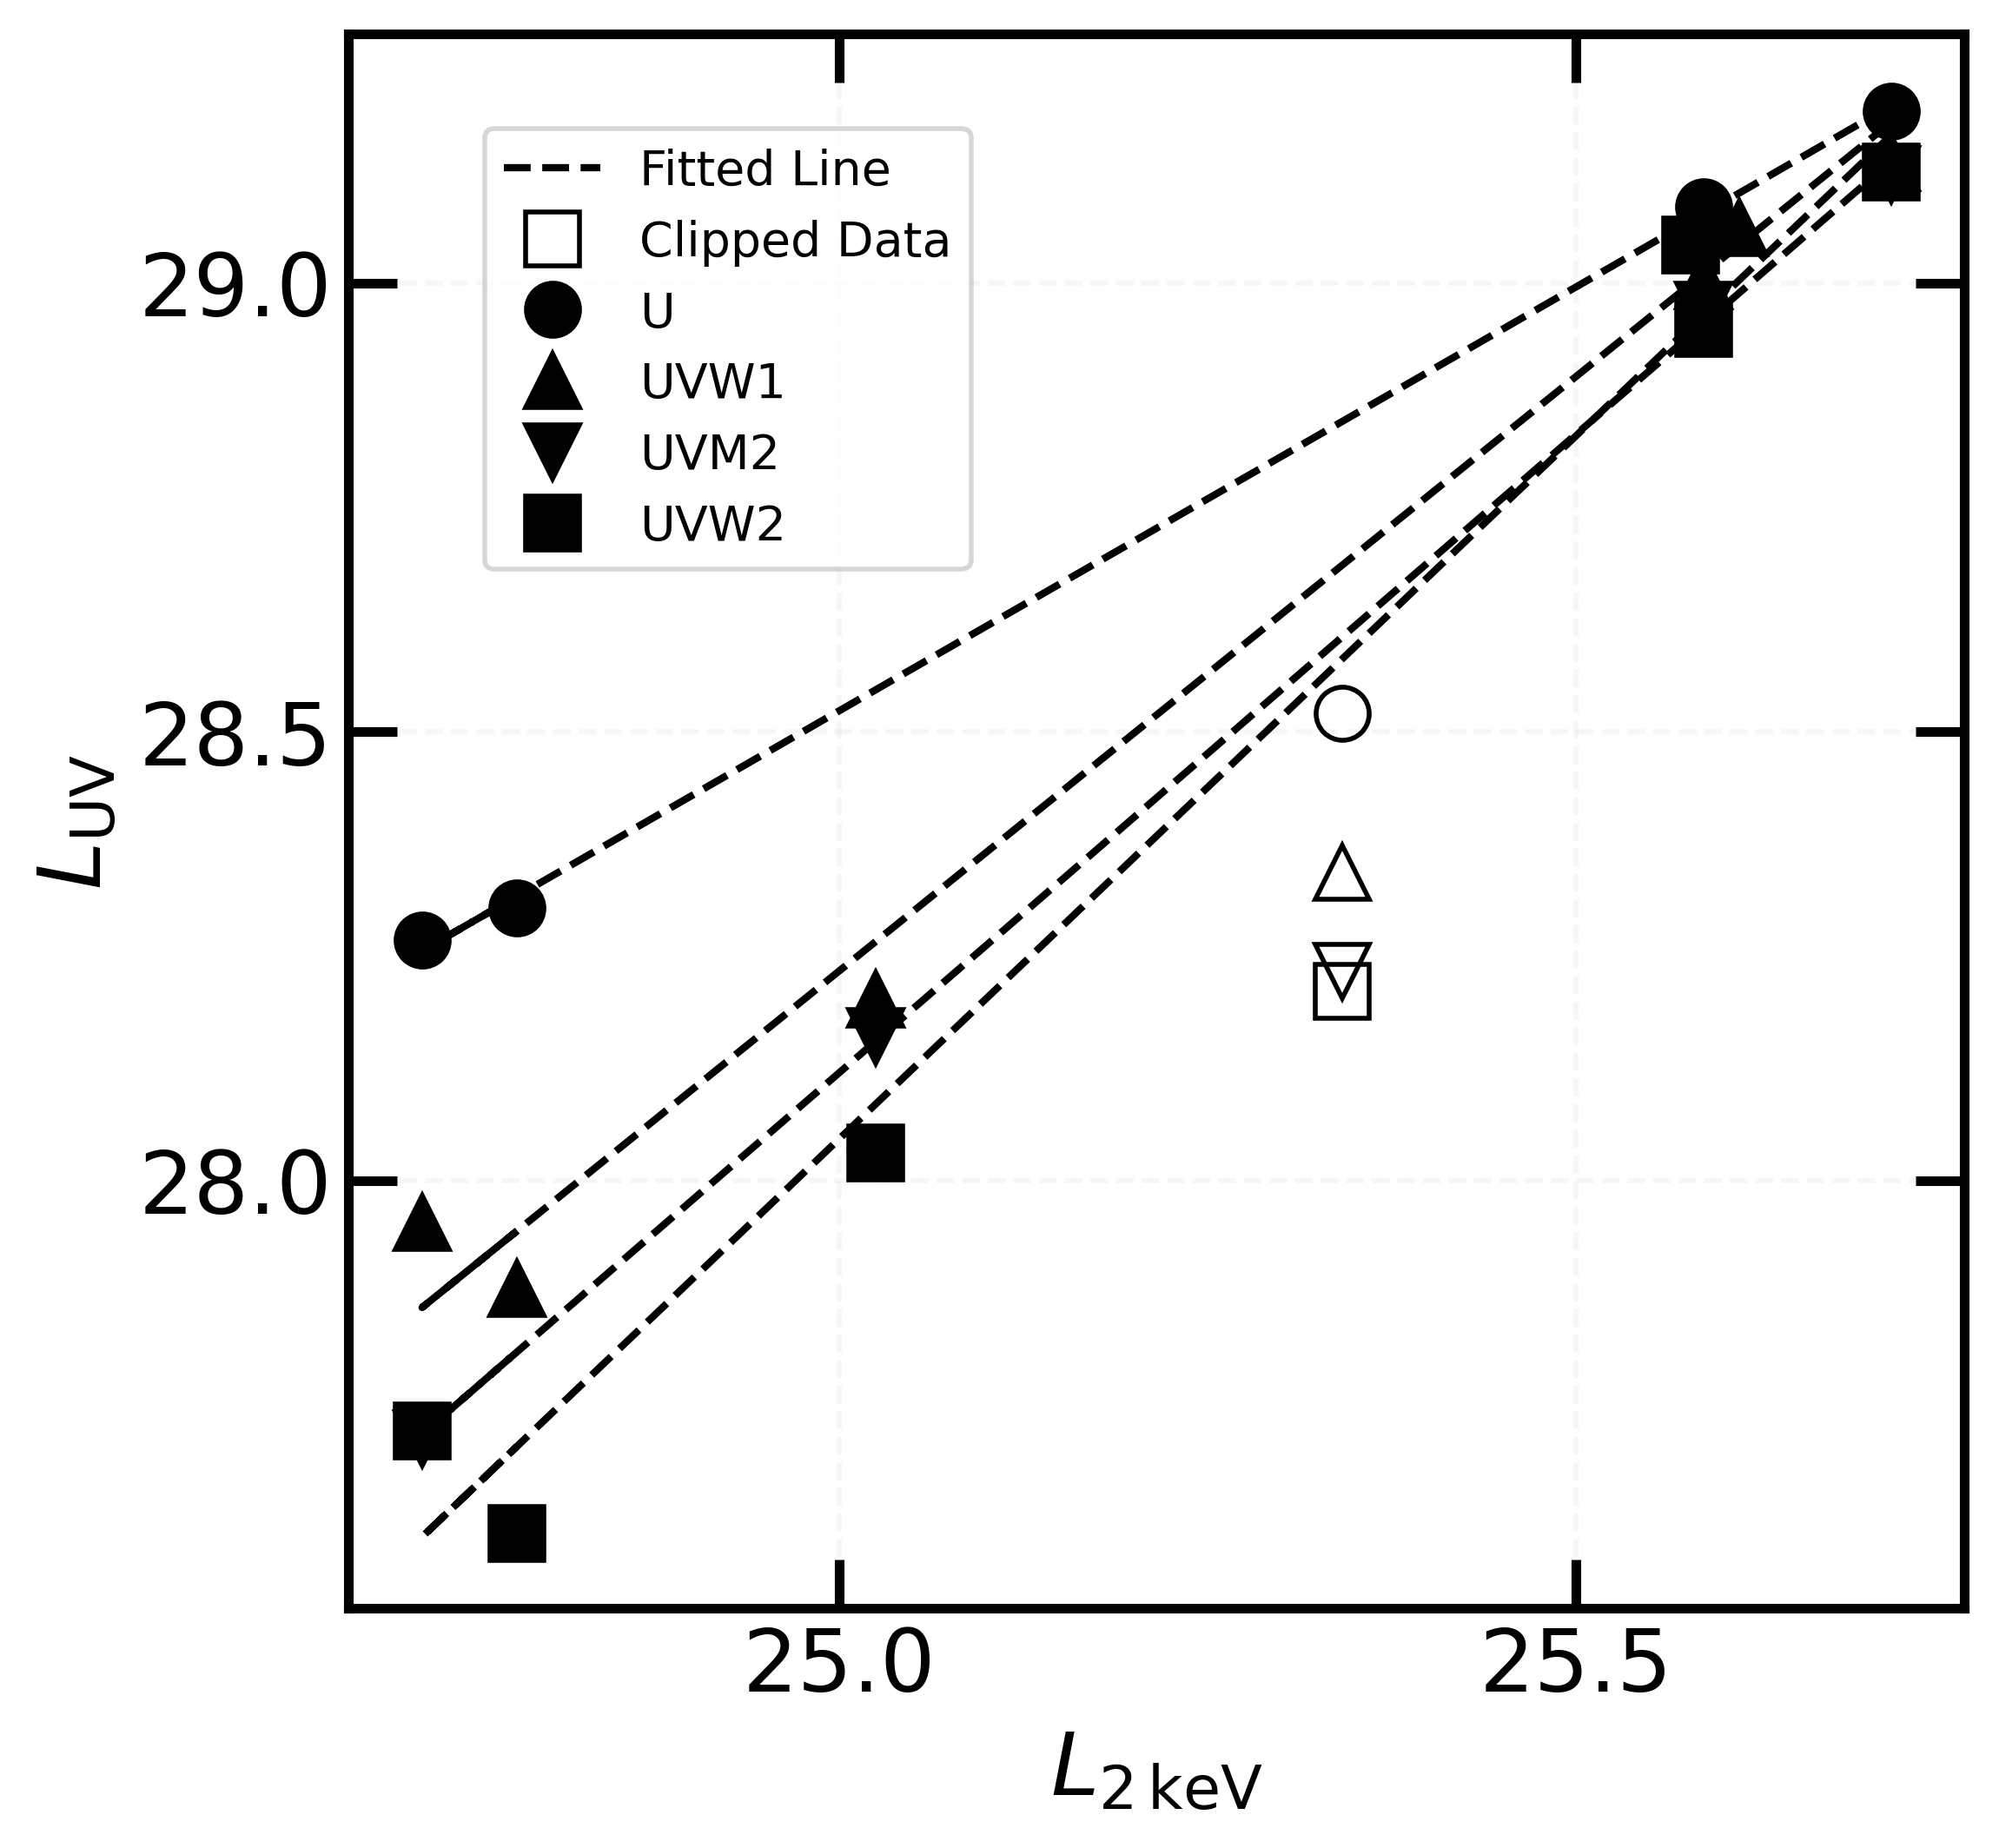
\includegraphics[width=0.6\textwidth]{./pic/Mrk1018_L2_Luvot_correlation-fig-without-outlier_clip.png}
    \caption{Correlation between $L_{UV}$ and $L_\mathrm{2\,keV}$ during 2005 and 2016. We clip the outlier data point in blank marker. }
    \label{fig:correlation-Luvot-L2keV}
\end{figure*}

\begin{figure*}
\centering
	% To include a figure from a file named example.*
	% Allowable file formats are eps or ps if compiling using latex
	% or pdf, png, jpg if compiling using pdflatex
	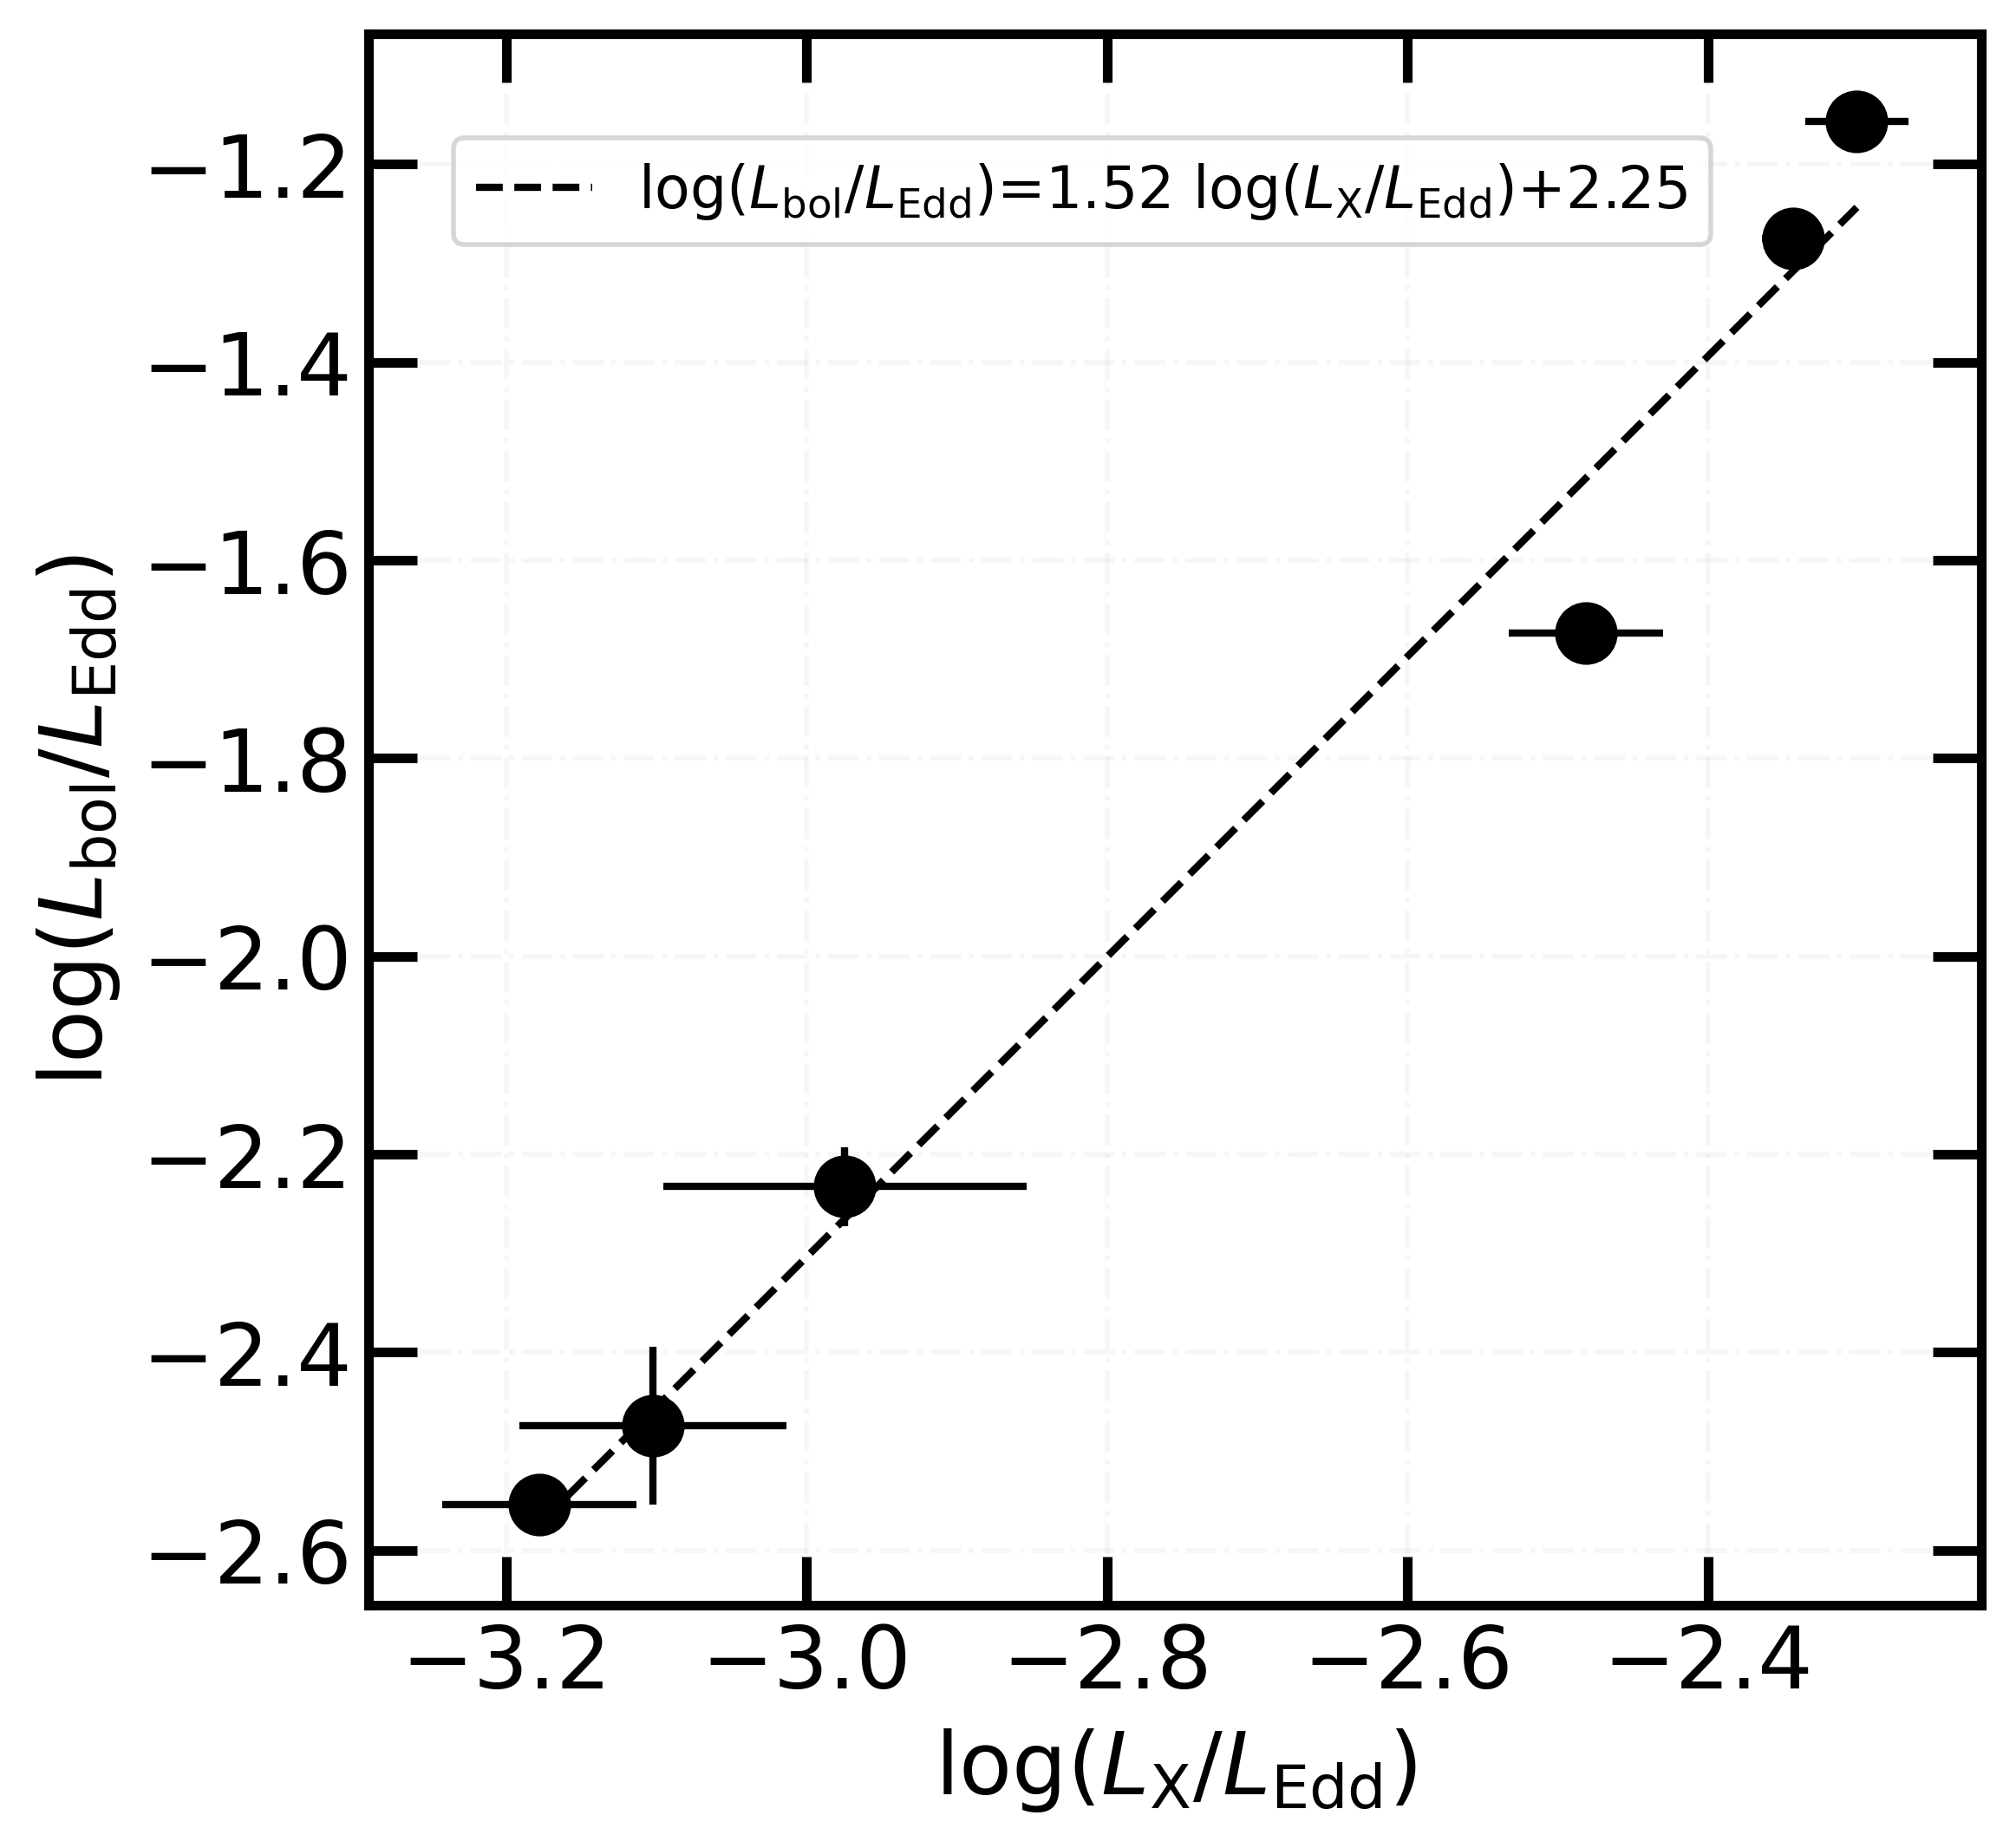
\includegraphics[width=0.6\textwidth]{./pic/Mrk1018_LxvsLBol_fit.png}
    \caption{$L_\mathrm{2-10\,keV}$ vs. bolometric luminosity $L_\mathrm{bol}$ for Mrk~1018. $L_\mathrm{bol}$ is estimated based on \texttt{optxagnf} model. Markers in circle, triangle and inverted-triangle represent that Mrk~1018 is at type 1, unknown, and type 1.9 state.}
    \label{fig:xray-bol}
\end{figure*}



\begin{figure*}
\centering
	% To include a figure from a file named example.*
	% Allowable file formats are eps or ps if compiling using latex
	% or pdf, png, jpg if compiling using pdflatex
	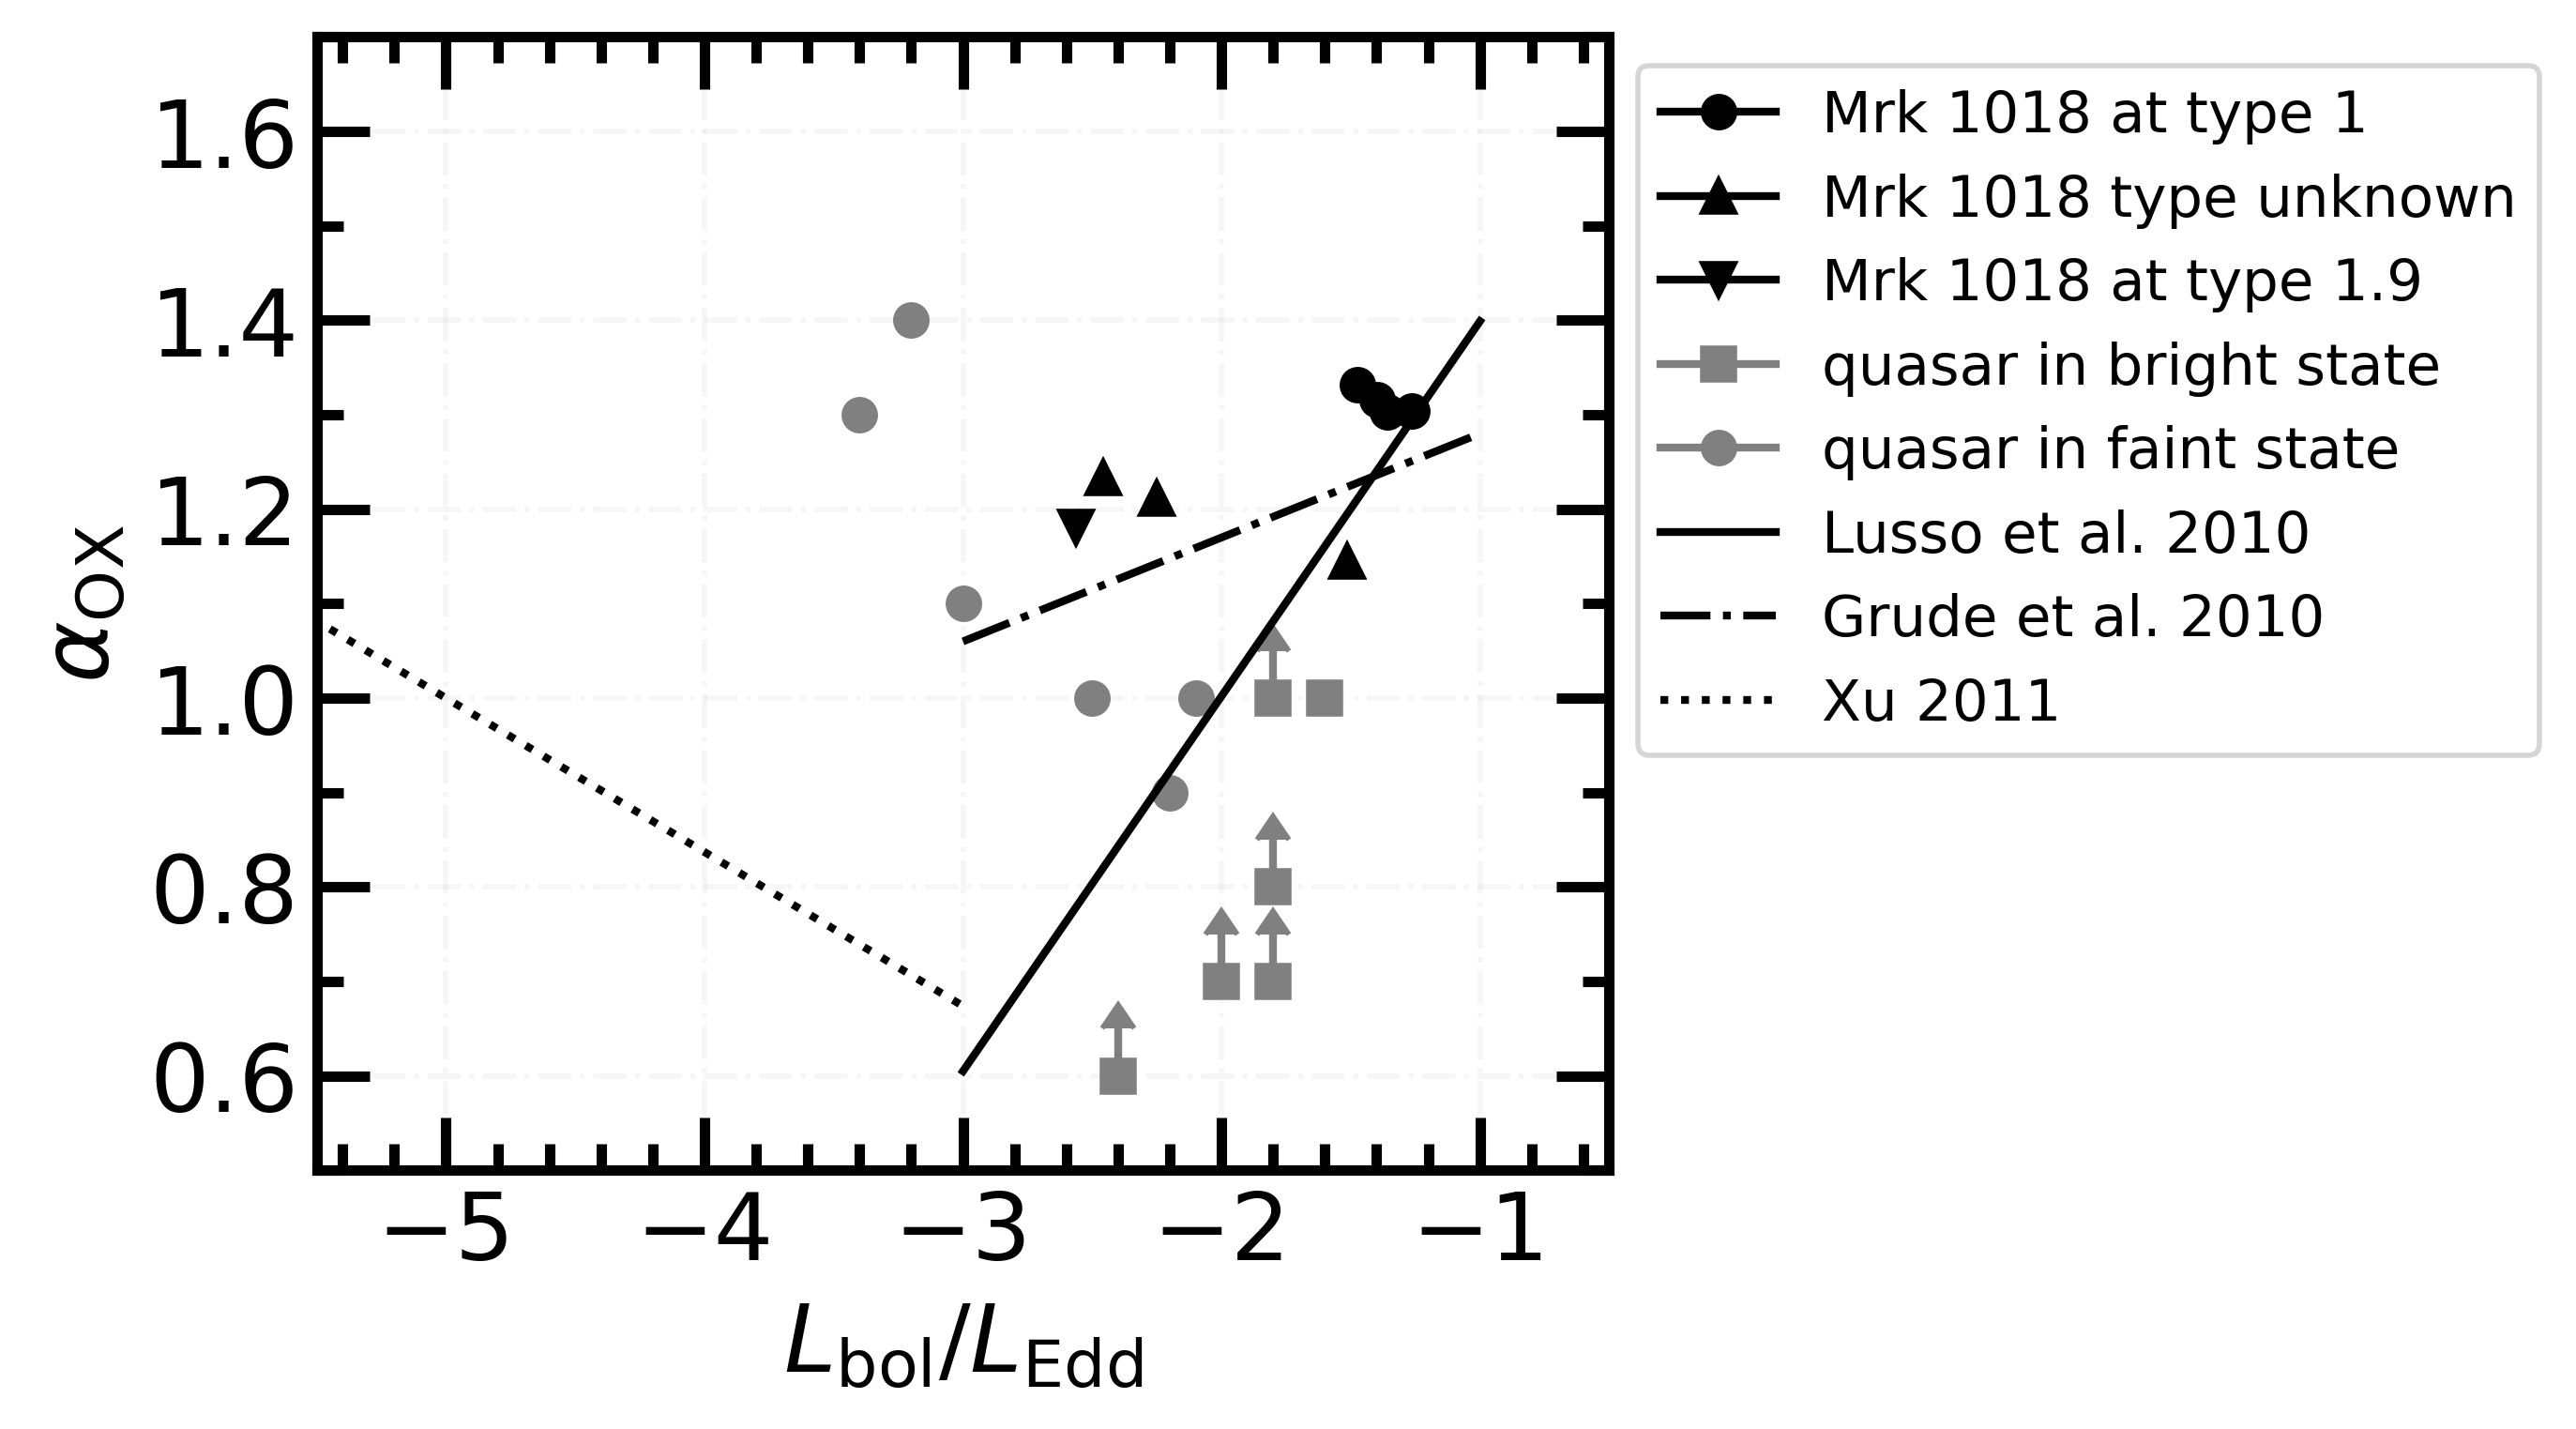
\includegraphics[width=0.9\textwidth]{./pic/Mrk1018_subplots_plus_alpha_ox_logLbol_rate.png}
    \caption{$\alpha_\mathrm{OX}$ vs. $L_\mathrm{bol}$ correlation for Mrk~1018 in comparison with other samples or best-fitting result such as low-luminosity Active Galactic Nuclei in \citet[][]{2011ApJ...739...64X}, type 1 AGN in \citet{2010A&A...512A..34L}, soft X-Ray selected Active Galactic Nuclei in \citet[][]{2010ApJS..187...64G} and Changing-look quasars in \citet[][]{2019ApJ...883...76R}. }
    \label{fig:alphaox-bol}
\end{figure*}


\begin{figure*}
\centering
	% To include a figure from a file named example.*
	% Allowable file formats are eps or ps if compiling using latex
	% or pdf, png, jpg if compiling using pdflatex
	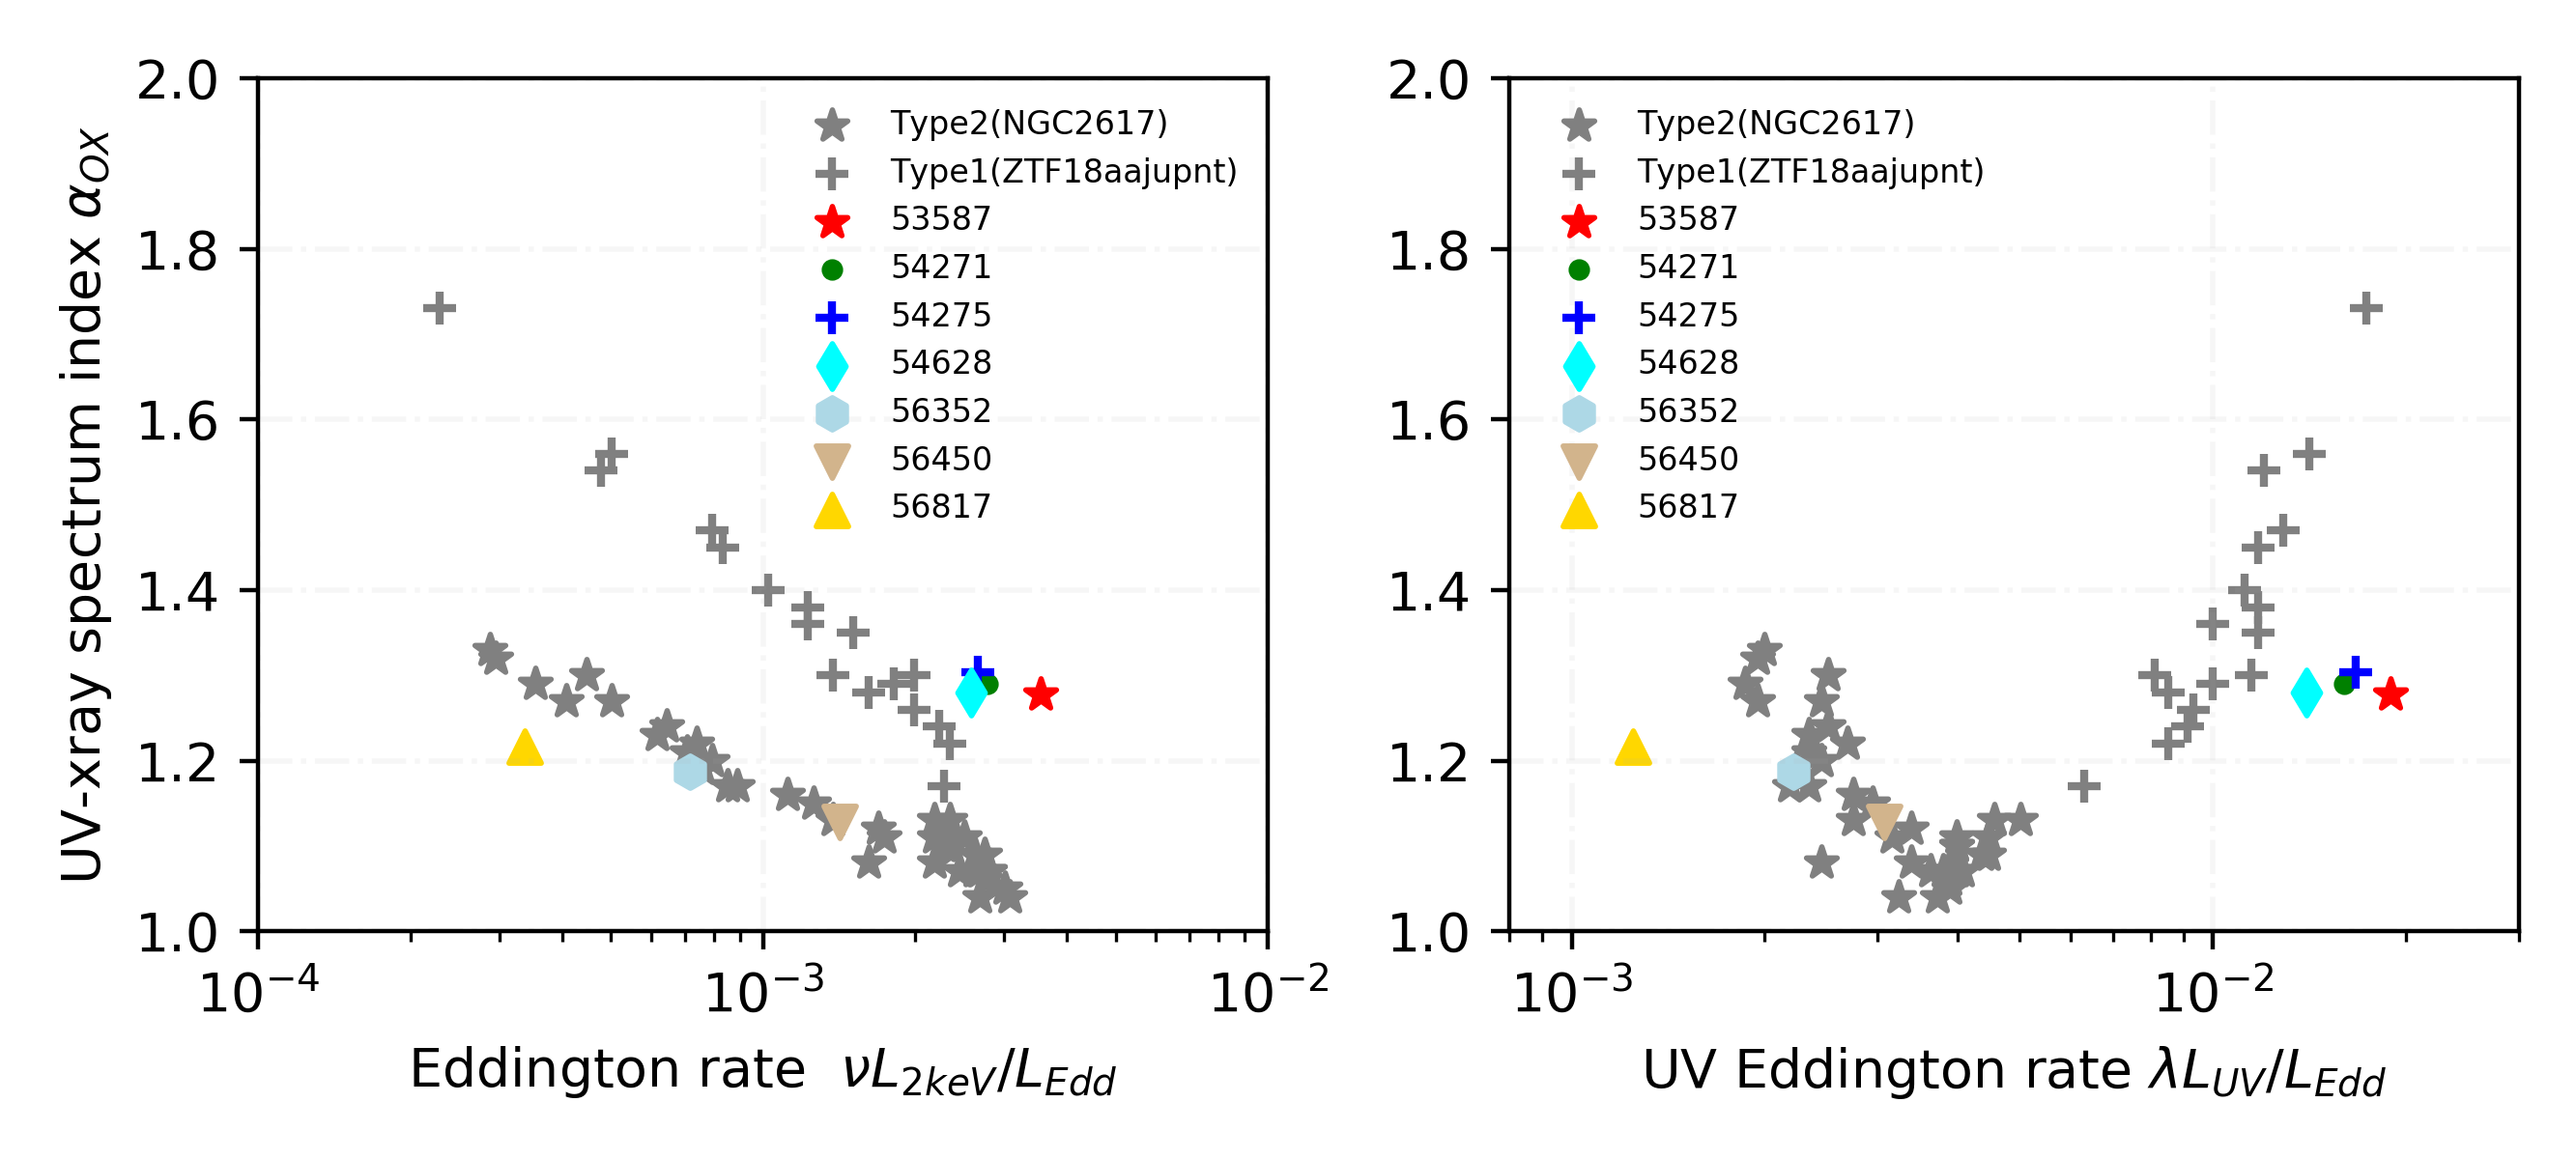
\includegraphics[width=0.9\textwidth]{./pic/Mrk1018_subplots_plus_2individuals_alpha_ox_L_x_Luv_rate.png}
    \caption{Mrk1018's $\alpha_\mathrm{OX}-\nu L_\mathrm{2keV}/L_\mathrm{Edd}$ and $\alpha_\mathrm{OX}-\lambda L_\mathrm{UV}/L_\mathrm{Edd}$ correlation in comparison with two CLAGNs in \citet{2019arXiv190904676R}.}   
    \label{fig:alpha_ox_lx_luv}
\end{figure*}

\begin{figure*}
\centering
	% To include a figure from a file named example.*
	% Allowable file formats are eps or ps if compiling using latex
	% or pdf, png, jpg if compiling using pdflatex
	
\includegraphics[width=0.7\textwidth]{./pic/xrayappendgood-errorbar-f-g-tmap.png}
    \caption{The photon index $\Gamma$ vs. the 2--10 keV X-ray flux for Mrk~1018. There is an apparent evolution with time. We find a re-flare  which transited from left branch to right branch of $\Gamma$-flux correlation in less than 100 days, which is marked by an arrow. }
    \label{fig:xrayappendgood-fandg-tmap}
\end{figure*}

\begin{figure*}
\centering
	% To include a figure from a file named example.*
	% Allowable file formats are eps or ps if compiling using latex
	% or pdf, png, jpg if compiling using pdflatex
	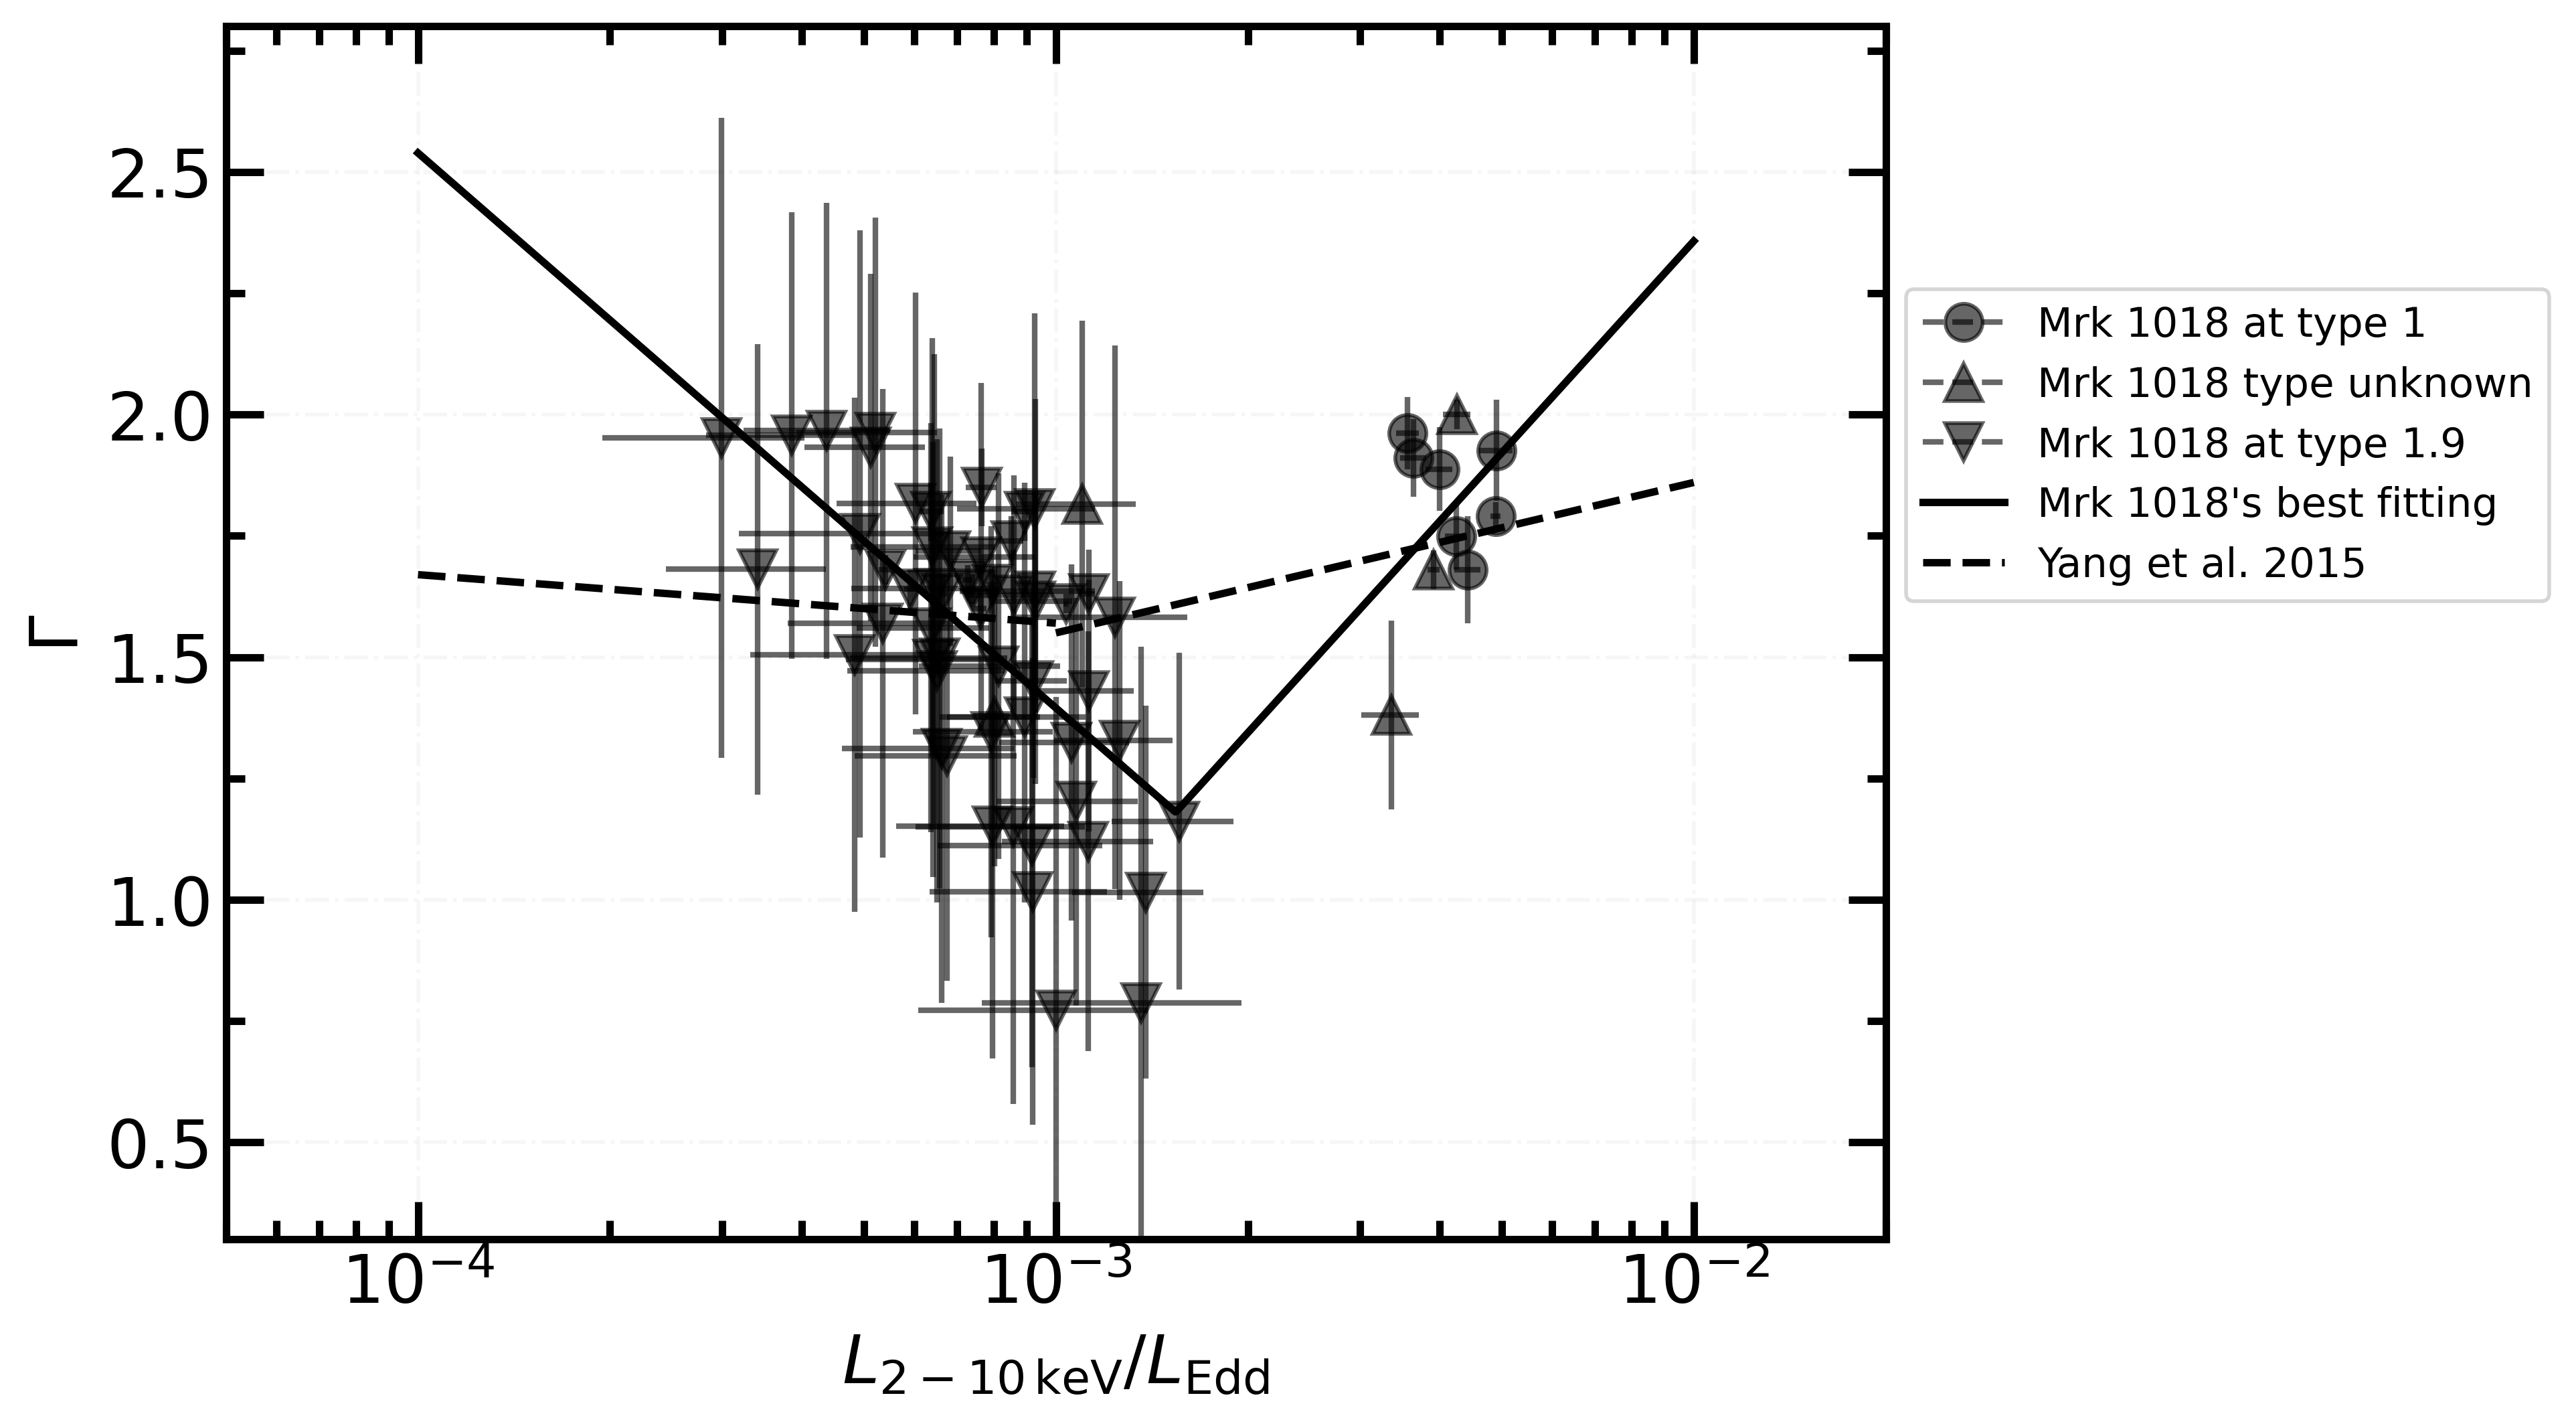
\includegraphics[width=0.7\textwidth]{./pic/xrayappendgood-errorbar-Lrate-g-tmap_brokenlinear_dot.png}
    \caption{$\Gamma$ vs. $L_\mathrm{2-10\,keV}/L_\mathrm{Edd}$ with best fitting shown in broken line. The critical value for log$L_\mathrm{2-10\,keV}/L_\mathrm{Edd}$ is $\sim$ -2.81. Dashed lines represent the results from \citet{2015MNRAS.447.1692Y} with critical value log$L_\mathrm{2-10\,keV}/L_\mathrm{Edd}$ $\sim$ -3. }
    \label{fig:xrayappendgood-Lrateandg-tmap}
\end{figure*}













\begin{figure*}
\centering
	% To include a figure from a file named example.*
	% Allowable file formats are eps or ps if compiling using latex
	% or pdf, png, jpg if compiling using pdflatex
	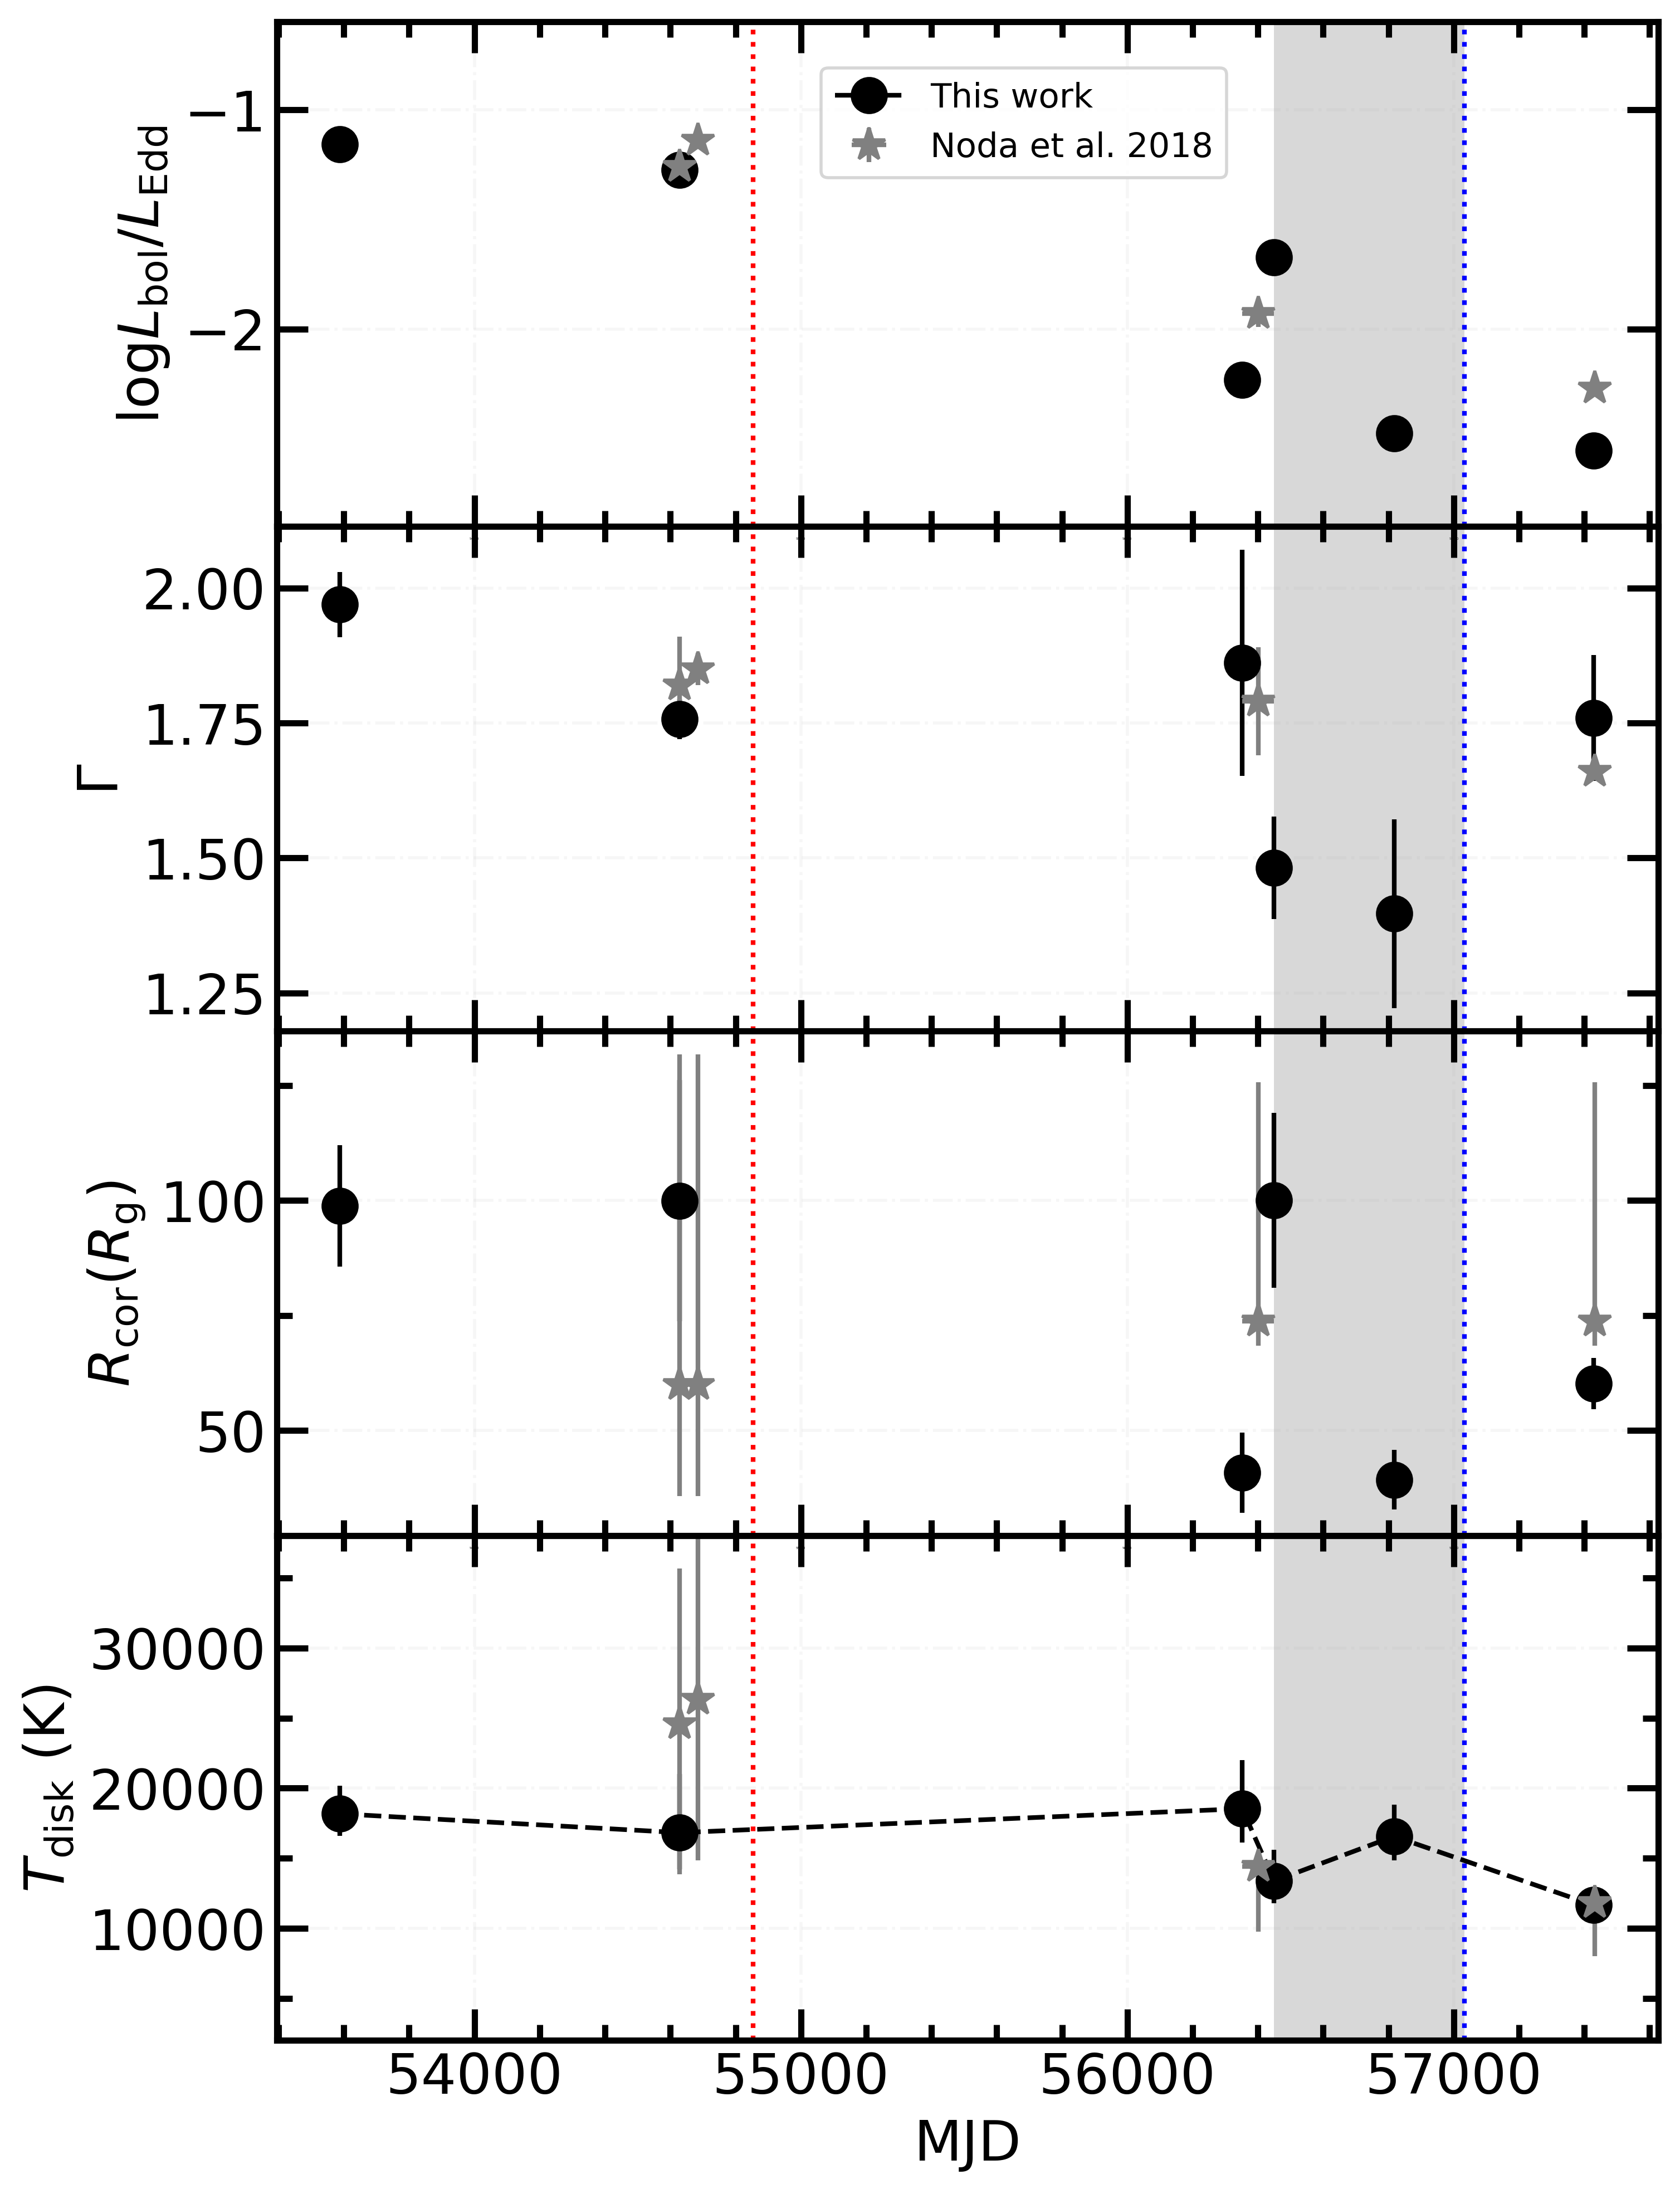
\includegraphics[width=0.9\textwidth]{./pic/Mrk1018_disk_time_evolution.png}
    \caption{The evolution of bolometric luminosity (log$L_\mathrm{bol}/L_\mathrm{Edd}$) based on \texttt{optxagnf} model, photon index ($\Gamma$), corona radius ($r_\mathrm{cor}$), and disk temperature ($T_\mathrm{disk}$) derived from log$L_\mathrm{bol}/L_\mathrm{Edd}$ and truncated disk radius ($r_\mathrm{tr}$) as same as $r_\mathrm{cor}$. Grey points represent results of joint fitting in \citep{2018MNRAS.480.3898N}. Black data points represent our fitting results with simultaneous \xrt\, and \uvot\, observation. Since \citep{2018MNRAS.480.3898N} combined data of 2013 and 2016 respectively, and fit all the four observations jointly, they got intermediate estimations of $L_\mathrm{bol}$ and $r_{cor}$ for observations in 2013 and 2016. Red and blue vertical dotted line represents the last time of optical spectroscopic confirmation at type 1 and type 1.9, respectively.}
    \label{fig:disk_evoliton}
\end{figure*}


\begin{figure*}
\centering
	% To include a figure from a file named example.*
	% Allowable file formats are eps or ps if compiling using latex
	% or pdf, png, jpg if compiling using pdflatex
	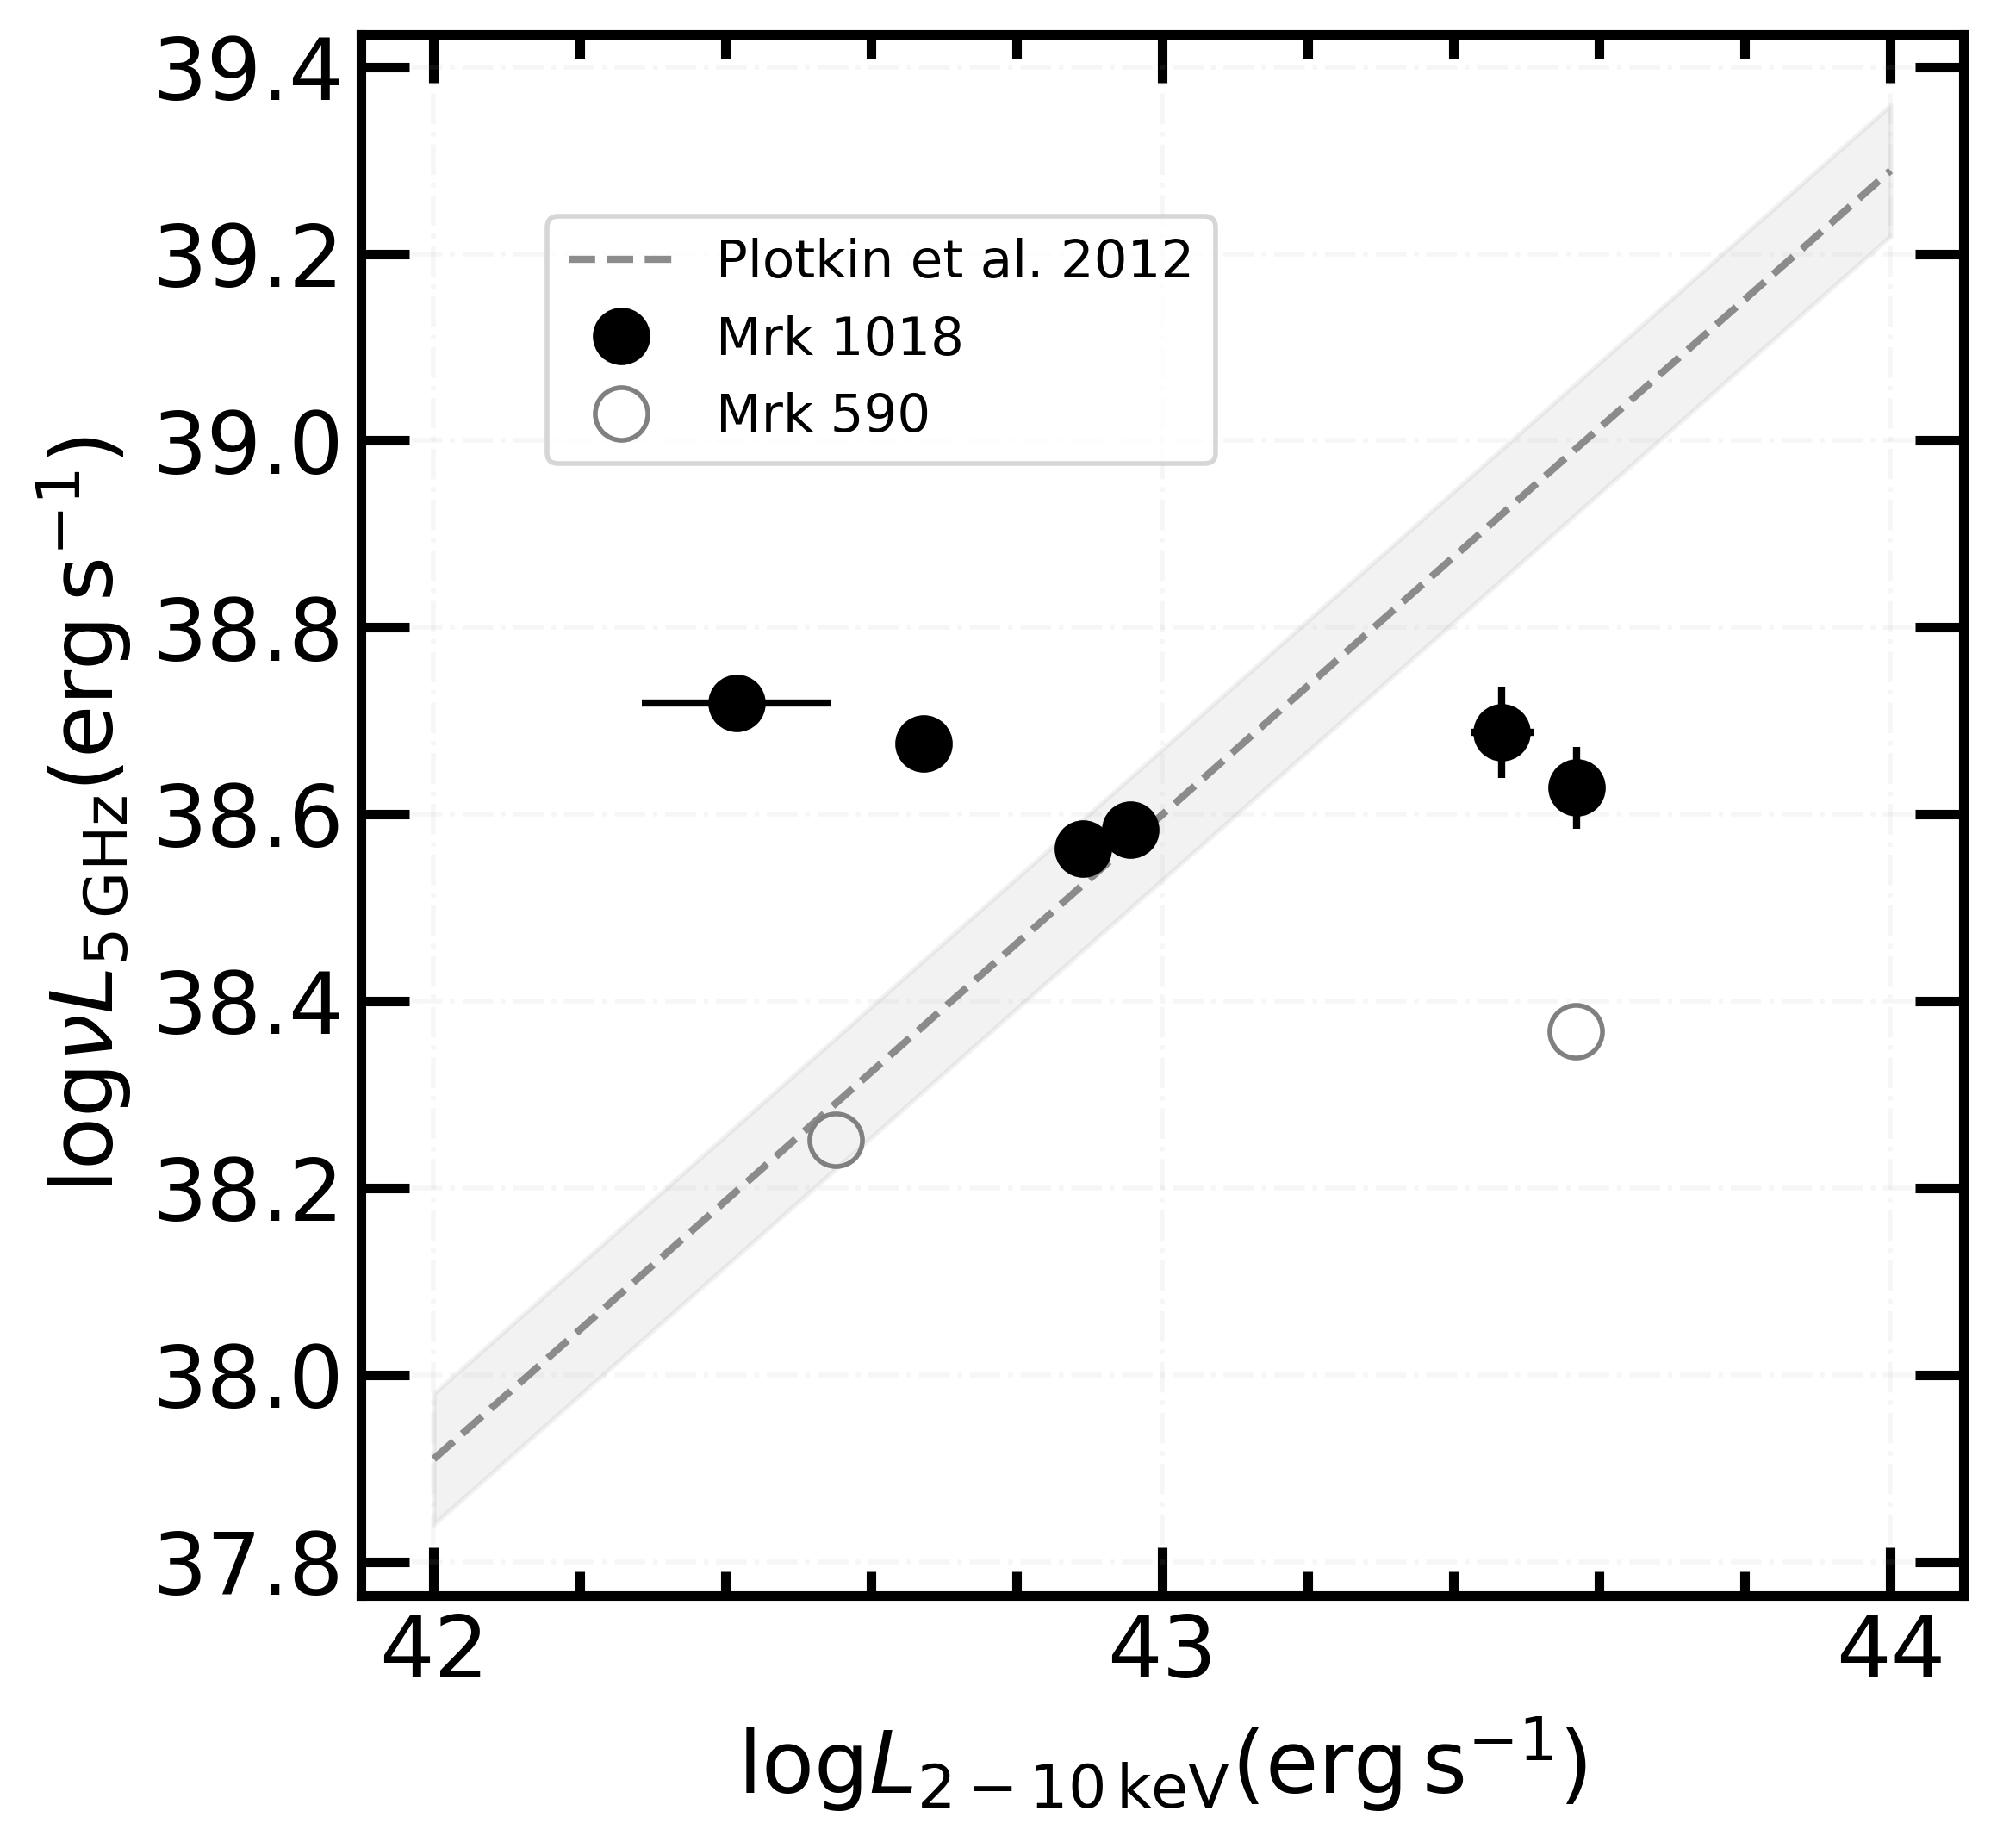
\includegraphics[width=0.6\textwidth]{./pic/Mrk1018_Mrk590_radio_xray_Plotkin2012_Lx.png}
    \caption{Mrk~1018's radio and X-ray luminosity relation relative to fundamental plane defined in \citet{2012MNRAS.419..267P} shown in grey straight line with intrinsic $\sigma=0.07$. We add the data of Mrk~590 from Table~5 in \citet{2016MNRAS.460..304K} for comparison.} 
    \label{fig:radio-xray-mass_relation_Plotkin2012}
\end{figure*}



%This work is supported by...
%% To help institutions obtain information on the effectiveness of their 
%% telescopes the AAS Journals has created a group of keywords for telescope 
%% facilities.
%
%% Following the acknowledgments section, use the following syntax and the
%% \facility{} or \facilities{} macros to list the keywords of facilities used 
%% in the research for the paper.  Each keyword is check against the master 
%% list during copy editing.  Individual instruments can be provided in 
%% parentheses, after the keyword, but they are not verified.




%% Appendix material should be preceded with a single \appendix command.
%% There should be a \section command for each appendix. Mark appendix
%% subsections with the same markup you use in the main body of the paper.

%% Each Appendix (indicated with \section) will be lettered A, B, C, etc.
%% The equation counter will reset when it encounters the \appendix
%% command and will number appendix equations (A1), (A2), etc. The
%% Figure and Table counter will not reset.

\clearpage
%\bibliographystyle{mnras}
\bibliography{refMrk1018}{}
% if your bibtex file is called example.bib
\bibliographystyle{aasjournal}
%\clearpage

\begin{table}
\centering
\caption{{ \bf X-ray fit parameters of Mrk~1018. } Columns include the date of the observation, the facility, observation id, reduced $\chi ^2$ of the best fit model, the photon index $\Gamma$ with 90\% uncertainty, and the flux in 2-10~keV after Galactic-absorption correction. }
\label{tab:table1}

\begin{tabular}{lcccccc}
\hline
\hline
 
  Date   &   Instrument & obsid  & $\chi ^2$  &$\Gamma$  &  $F_{2-10keV}$  & \\ 
  (MJD)  &              &        &          &                    &  [erg cm$^{-2}$ s$^{-1}$] &      
 \\  \hline
53385 & X & 201090201 & 0.98 & 1.73 $\pm$ 0.07 & 9.7e-12 $\pm$ 6e-13 \\ 
53587 & S & 35166001 & 0.78 & 1.93 $\pm$ 0.1 & 1.15e-11 $\pm$ 6.99e-13 \\ 
54271 & S & 30955001 & 1.01 & 1.89 $\pm$ 0.09 & 9.39e-12 $\pm$ 4.47e-13 \\ 
54274 & S & 30955002 & 1.07 & 1.91 $\pm$ 0.08 & 8.54e-12 $\pm$ 4e-13 \\ 
54276 & S & 30955003 & 1.02 & 1.96 $\pm$ 0.08 & 8.38e-12 $\pm$ 3.47e-13 \\ 
54628 & S & 35776001 & 1.19 & 1.75 $\pm$ 0.07 & 9.98e-12 $\pm$ 3.96e-13 \\ 
54685 & X & 554920301 & 1.16 & 1.79 $\pm$ 0.02 & 1.13e-11 $\pm$ 2e-13 \\ 
55527$^{(a)}$ & C & 12868 & 1.1 & 1.7 $\pm$ 0.03 & 9.26e-12 $\pm$ 1.9e-13 \\ 
56353 & S & 49654001 & 1.42 & 1.82 $\pm$ 0.38 & 2.59e-12 $\pm$ 5.52e-13 \\ 
56450 & S & 49654002 & 1.23 & 1.38 $\pm$ 0.19 & 7.9e-12 $\pm$ 8.21e-13 \\ 
56818 & S & 49654004 & 0.75 & 1.38 $\pm$ 0.31 & 1.88e-12 $\pm$ 3.37e-13 \\ 
57428 & N & 60160087002 & 1.23 & 1.85 $\pm$ 0.08 & 1.8e-12 $\pm$ 1e-13 \\ 
57429 & S & 80898001 & 0.96 & 1.72 $\pm$ 0.2 & 1.61e-12 $\pm$ 1.89e-13 \\ 
57434 & S & 80898002 & 0.9 & 1.45 $\pm$ 0.2 & 2.17e-12 $\pm$ 2.77e-13 \\ 
57443 & C & 18789 & 0.82 & 1.7 $\pm$ 0.03 & 1.3e-12 $\pm$ 3e-14 \\ 
57801 & C & 19560 & 1.26 & 1.61 $\pm$ 0.02 & 2.48e-12 $\pm$ 4e-14 \\ 
58123 & N & 60301022002 & 1.34 & 1.8 $\pm$ 0.06 & 2.1e-12 $\pm$ 1e-13 \\ 
58125 & S & 88207001 & 1.04 & 1.63 $\pm$ 0.25 & 2.02e-12 $\pm$ 3.08e-13 \\ 
58126 & C & 20366 & 1.05 & 1.6 $\pm$ 0.03 & 1.84e-12 $\pm$ 5e-14 \\ 
58180 & C & 20367 & 1.02 & 1.61 $\pm$ 0.04 & 1.59e-12 $\pm$ 5e-14 \\ 
58182 & N & 60301022003 & 1.03 & 1.8 $\pm$ 0.06 & 1.5e-12 $\pm$ 7e-14 \\ 
58281 & C & 20368 & 1.02 & 1.62 $\pm$ 0.03 & 1.77e-12 $\pm$ 5e-14 \\ 
58316 & N & 60301022005 & 0.85 & 1.74 $\pm$ 0.05 & 2e-12 $\pm$ 9e-14 \\ 
58317 & S & 88207003 & 1.01 & 1.61 $\pm$ 0.23 & 2.18e-12 $\pm$ 3.12e-13 \\  \\ \hline
\end{tabular}\\
Notes: Here the superscripts $^{(a)}$ represents fit result that are taken from \citet{2017A&A...607L...9K}. Instrument indicate by C-\chandra, S-\swift, X-\xmm, N-\nustar. 
\end{table}
\clearpage
%






\begin{table}
\centering
\caption{{\bf $\alpha_{ox}$ of Mrk~1018 with simultaneous XRT and UVOT observation.} Columns include the date of the observation, $\alpha_{ox}$, flux in 2-10~keV, $\nu F_{uw1}$, and Eddington rate.}
\label{tab:tablealpha_ox}
\begin{tabular}{lcccccc}
\hline
\hline
 
 Date &   $\alpha_{ox}$  & $F_{2-10keV}$  &$\nu F_{uw1}$  & $L_{2-10keV}/L_{Edd}$ &   $\nu L_{uw1}/L_{Edd}$  \\ 
 (MJD)&                   &   [erg cm$^{-2}$ s$^{-1}$]   &[erg cm$^{-2}$ s$^{-1}$]    &                    &            
 \\ \hline
53587 & 1.29 & 1.14e-11 & 3.92e-11 & 5.53e-03 & 1.90e-02 \\ 
54271 & 1.30 & 9.34e-12 & 3.31e-11 & 4.51e-03 & 1.60e-02 \\ 
54275 & 1.31 & 8.78e-12 & 3.45e-11 & 4.24e-03 & 1.67e-02 \\ 
54628 & 1.29 & 9.85e-12 & 2.89e-11 & 4.76e-03 & 1.40e-02 \\ 
56352 & 1.20 & 2.59e-12 & 4.58e-12 & 1.25e-03 & 2.22e-03 \\ 
56450 & 1.14 & 8.26e-12 & 6.35e-12 & 3.99e-03 & 3.07e-03 \\ 
56817 & 1.23 & 1.98e-12 & 2.58e-12 & 9.57e-04 & 1.25e-03 \\ \hline
\end{tabular}   
\end{table}
\begin{table}
\centering
\caption{{\bf VLA observation of Mrk~1018.} Columns include the date of observation, project name, band, frequency, integrated flux, radio spectral index ($\alpha$) and reference.}
\label{tab:tableradio}
\begin{tabular}{lcccccr}
\hline
\hline
 
 Date &  project & band  & Frequency  &$F_{int}$   & $\alpha$ & Reference  \\ 
 (MJD)&         &        &   [GHz]   &[mJy]     &                &         \\ \hline
    \multirow{2}*{46032} & \multirow{2}*{AU0020} & L    & 1.49  & 4.21  $\pm$ 0.23  & \multirow{2}*{0.52 $\pm0.07$} &\\
    \,          &        & C     & 4.86  & 2.29  $\pm$ 0.14  & & \\
    47261     & AB0476 & C     & 4.86  & 1.91  $\pm$ 0.23  &  &\\
    47692     & AB0540A & C     & 4.86  & 2.62  $\pm$ 0.16  &  &\\
    47732     & AB0540B & C     & 4.86  & 2.31  $\pm$ 0.17  & & \\
    49820.5 $\pm$ 773.5 & AB0628 & L     & 1.4   & 4.20  $\pm$ 0.45  &  & \citet{1998AJ....115.1693C} \\
    49820.5 $\pm$ 773.5 & AB0628 & L     & 1.4   & 4.15  $\pm$ 0.25  &  & \citet{1997ApJ...475..479W} \\
    50219.5 $\pm$ 1078.5 & AB0308 & L     & 1.4   & 4.20  $\pm$ 0.54  &  & \citet{2002AJ....124..675C}\\
    50970     & AB0878 & X     & 8.46  & 2.47  $\pm$ 0.17  & 0.3 $\pm0.08$\\
    52246.5 $\pm$ 278.5 & AB0950 & L     & 1.4   & 4.15  $\pm$ 0.25  & & \citet{2003yCat.8071....0B} \\
    54872.5 $\pm$ 51.5  & AR685 & L     & 1.4   & 3.69  $\pm$ 0.19  &  & \citet{2011AJ....142....3H}\\
    54878   & AB1314 & L     & 1.4   & 3.36  $\pm$ 0.20  &  & \citet{2012yCat.8090....0B} \\
    56550 $\pm$ 8     & 13B-272 & L     & 1.4   & 3.85  $\pm$ 0.31  &  & \citet{2016MNRAS.460.4433H} \\

    \multirow{3}*{57481}     &  \multirow{3}*{16A-444} & C     & 5     & 2.56  $\pm$ 0.13  & \multirow{3}*{0.02$\pm0.05$}& \\
              &     & X     & 10    & 2.16  $\pm$ 0.11  & &\\
              &    &  K     & 22    & 2.46  $\pm$ 0.12  &  &\\
    57719     & 16B-084 & X     & 10    & 1.78  $\pm$ 0.09  &   &\\

    57731     & 16B-084 & X     & 10    & 1.97  $\pm$ 0.10  &  &\\

    57768     & 16B-084 & C     & 5     & 2.07  $\pm$ 0.10  & 0 &\\
    58087     & VLASS1.1 & L     & 3     & 2.30  $\pm$ 0.36  & & \\
    
    58472     & 18B-245 & K     & 20    & 2.71  $\pm$ 0.14  &  & \\



\hline 
\end{tabular}   
\end{table}




     
\begin{table}
\centering
\caption{{\bf Radio and X-ray luminosity diagram.} Columns include the date of the radio observation, the radio spectrum index $\alpha_{radio}$, the date of X-ray observation, the interval between two bands, the flux and luminosity rescaled to 4.8 and 8.4~GHz, the X-ray flux and luminosity in 2-10~keV band.}
\label{tab:table4}
\begin{tabular}{lllllllllr}
\hline
\hline

$T_{Radio}$ &  $\alpha_{Radio}$ & $T_{X-ray}$ & $\delta$ T & $F_{2-10keV}$ & $F_{4.8GHz}$ & $F_{8.4GHz}$ &  $\nu L_{\nu=4.8GHz}$ &  $\nu L_{\nu=8.4GHz}$ & $L_{\rm{2--10~keV}}$ \\ 
(MJD)  &  & (MJD)  &(day)  &[erg$~s^{-1}~\rm{cm}^{-2}$] & [mJy)& (mJy)]& [erg$~s^{-1} $] & [erg$~s^{-1} $]& [erg$~s^{-1} $]\\
\hline

52246.5 & 0.42 & 53385 & 1138 & 9.70e-12 & 2.47 & 1.96 & 5.00e38 & 6.92e38 & 4.09e43 \\ 
54318 & 0.42 & 54276 & 42 & 8.78e-12 & 2.00 & 1.58 & 4.05e38 & 5.60e38 & 3.70e43 \\ 
54872.5 & 0.42 & 54685 & 188 & 1.13e-11 & 2.20 & 1.74 & 4.45e39 & 6.15e39 & 4.76e44 \\ 
56550 & 0.42 & 56450 & 100 & 8.26e-12 & 2.29 & 1.81 & 4.64e40 & 6.42e40 & 3.48e45 \\ 
57481 & 0.17 & 57443 & 38 & 1.30e-12 & 2.49 & 2.27 & 5.04e41 & 8.02e41 & 5.48e45 \\ 
57768 & 0.17 & 57801 & 33 & 2.48e-12 & 2.00 & 1.82 & 4.05e42 & 6.45e42 & 1.04e47 \\  \hline
\end{tabular}\\
Notes: We assume the $\alpha_{Radio}$ before/after the type transition as a constant, respectively. 
\end{table}


%\appendix
%\section{Appendix}


%\clearpage


%\clearpage


%% For this sample we use BibTeX plus aasjournals.bst to generate the
%% the bibliography. The sample63.bib file was populated from ADS. To
%% get the citations to show in the compiled file do the following:
%%
%% pdflatex sample63.tex
%% bibtext sample63
%% pdflatex sample63.tex
%% pdflatex sample63.tex




%% This command is needed to show the entire author+affiliation list when
%% the collaboration and author truncation commands are used.  It has to
%% go at the end of the manuscript.
%\allauthors

%% Include this line if you are using the \added, \replaced, \deleted
%% commands to see a summary list of all changes at the end of the article.
%\listofchanges
% Don't change these lines
%\bsp	% typesetting comment
%\label{lastpage}
\end{document}

% End of file `sample63.tex'.
